\documentclass[../main/main.tex]{subfiles}

\raggedbottom

\makeatletter
\renewcommand{\@chapapp}{M\'ecanique -- chapitre}
\makeatother

% \toggletrue{student}

\begin{document}
\setcounter{chapter}{6}

\chapter{Mouvement \`a force centrale conservative}

\section{Forces centrales conservatives}
\subsection{Force centrale}
\begin{tdefi}{Définition~: force centrale}
    Une force $\Ff$ est dite \textbf{centrale} s'il existe un point O fixe (dans
    $\Rc$) tel que $\Ff$ soit colinéaire à $\OM$ pour tout point M~; O est alors
    appelé \textbf{centre de force}. Autrement dit, $\Ff$ est centrale si sa
    direction est toujours celle de $\OM$. \smallbreak
    \begin{side}
        \begin{center}
            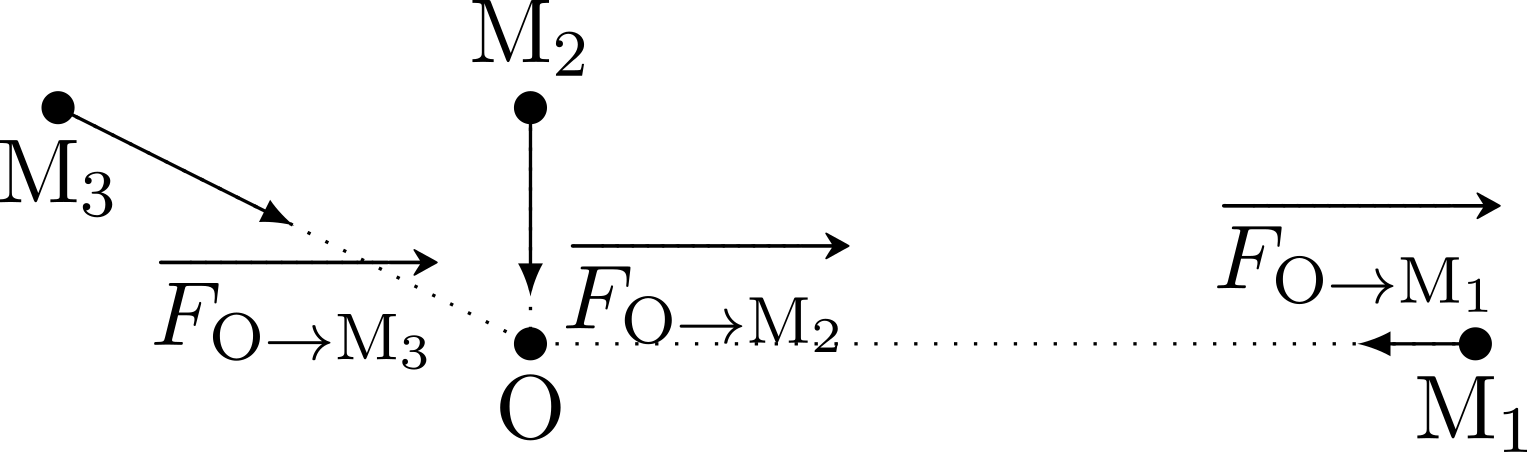
\includegraphics[width=\linewidth]{intro_att}
            Cas attractif
        \end{center}
        \tcblower
        \begin{center}
            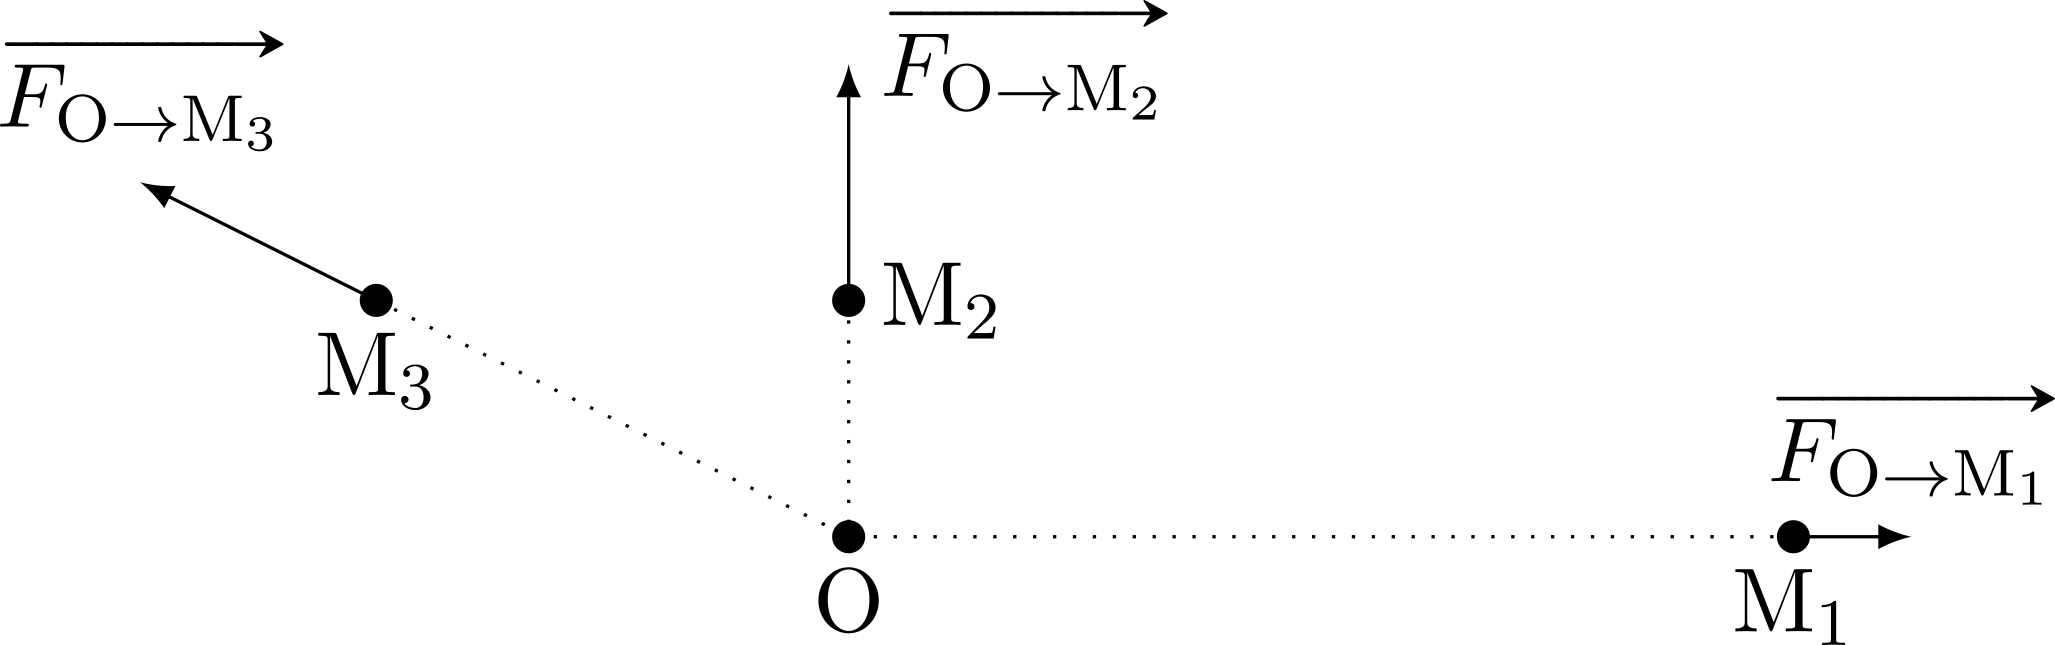
\includegraphics[width=\linewidth]{intro_rep}
            Cas répulsif
        \end{center}
    \end{side}
\end{tdefi}
\begin{rexem}{Exemples}
    \begin{itemize}
        \item Force d'attraction gravitationnelle~: \smallbreak
            \begin{minipage}{0.45\linewidth}
                \[\Ff_g = -\Gc \frac{m_\Or m}{r^2}\ur\]
            \end{minipage}
            \hfill
            \begin{minipage}{0.45\linewidth}
                \begin{center}
                    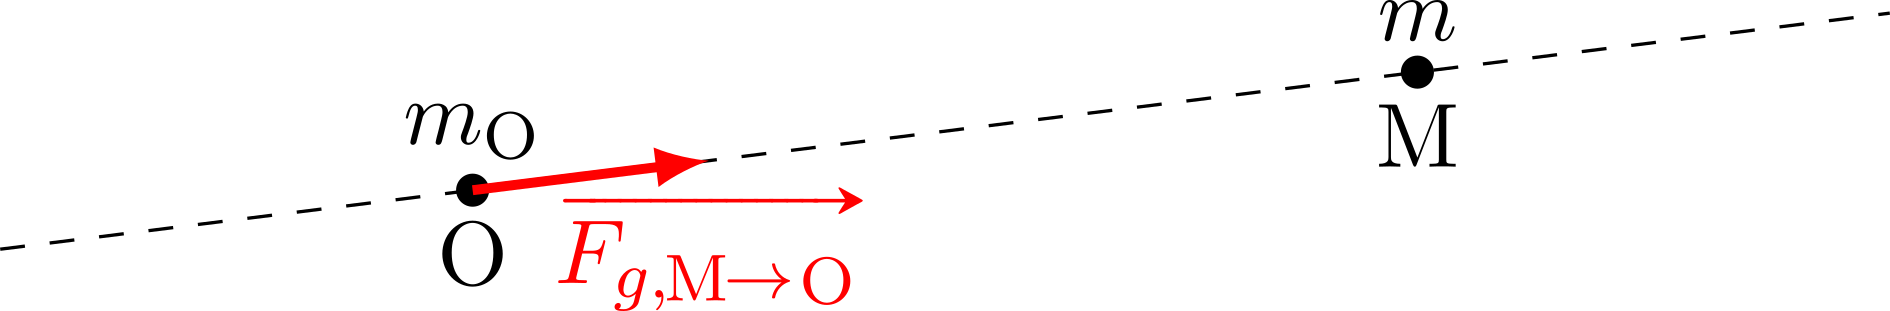
\includegraphics[scale=1]{intro_ex-grav}
                \end{center}
            \end{minipage}
        \item Force couloumbienne~: \smallbreak
            \begin{minipage}{0.45\linewidth}
                \[\Ff_e = \frac{1}{4\pi\ep_0} \frac{qq_\Or}{r^2}\ur\]
            \end{minipage}
            \hfill
            \begin{minipage}{0.45\linewidth}
                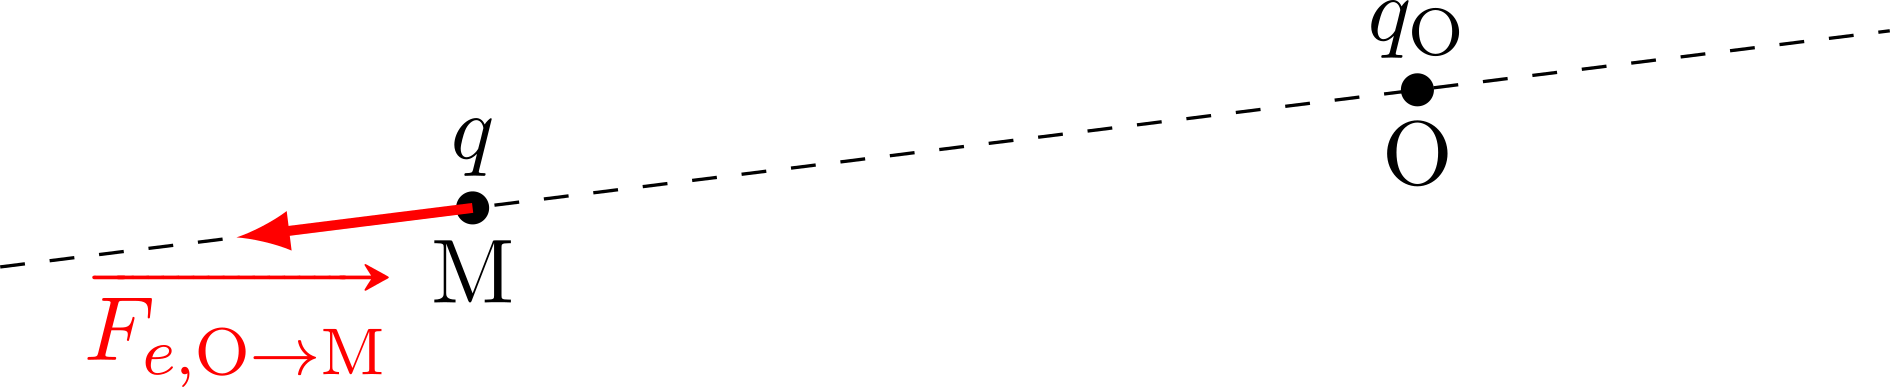
\includegraphics[scale=1]{intro_ex-elec}
            \end{minipage}
    \end{itemize}
\end{rexem}

\subsection{Force centrale conservative}
Plaçons-nous le plan contenant $\OM$ dans un repère polaire centré en O. Par
définition d'une force centrale, on a
\[\Ff = F(\Mr)\ur\]
et par définition d'une force conservative, on a
\begin{gather*}
    \de W(\Ff) = -\dd\Ec_p
    \Lra
    \Ff\cdot\dd{\OM} = -\dd{\Ec_p}
    \shortintertext{ou, de manière équivalente,}
    \Ff = -\gd\Ec_p
    \Lra
    \left\{
        \begin{aligned}
            F(\Mr) &= - \pdv{\Ec_p}{r}\\
            0 &= -\frac{1}{r}\pdv{\Ec_p}{\tt}\\
            0 &= -\pdv{\Ec_p}{z}\\
        \end{aligned}
    \right.
\end{gather*}
Ainsi, $\Ec_p$ ne dépend ni de $\tt$ ni de $z$, donc dépend uniquement de la
coordonnée $r$.

\begin{rexem}{Exemples}
    \begin{itemize}
        \item Interaction gravitationnelle~: \smallbreak
            \begin{minipage}{0.45\linewidth}
                \begin{align*}
                    -\pdv{\Ec_p}{r} &= -\Gc \frac{m_\Or m}{r^2}
                    \\\Lra
                    \Ec_p &= -\Gc \frac{m_\Or m}{r} + K
                    \\\Lra
                    \Aboxed{\Ec_p &= -\Gc \frac{m_\Or m}{r}}
                \end{align*}
                en fixant par convention $\Ec_p(+\infty) = 0$.
            \end{minipage}
            \hfill
            \begin{minipage}{0.45\linewidth}
                \begin{center}
                    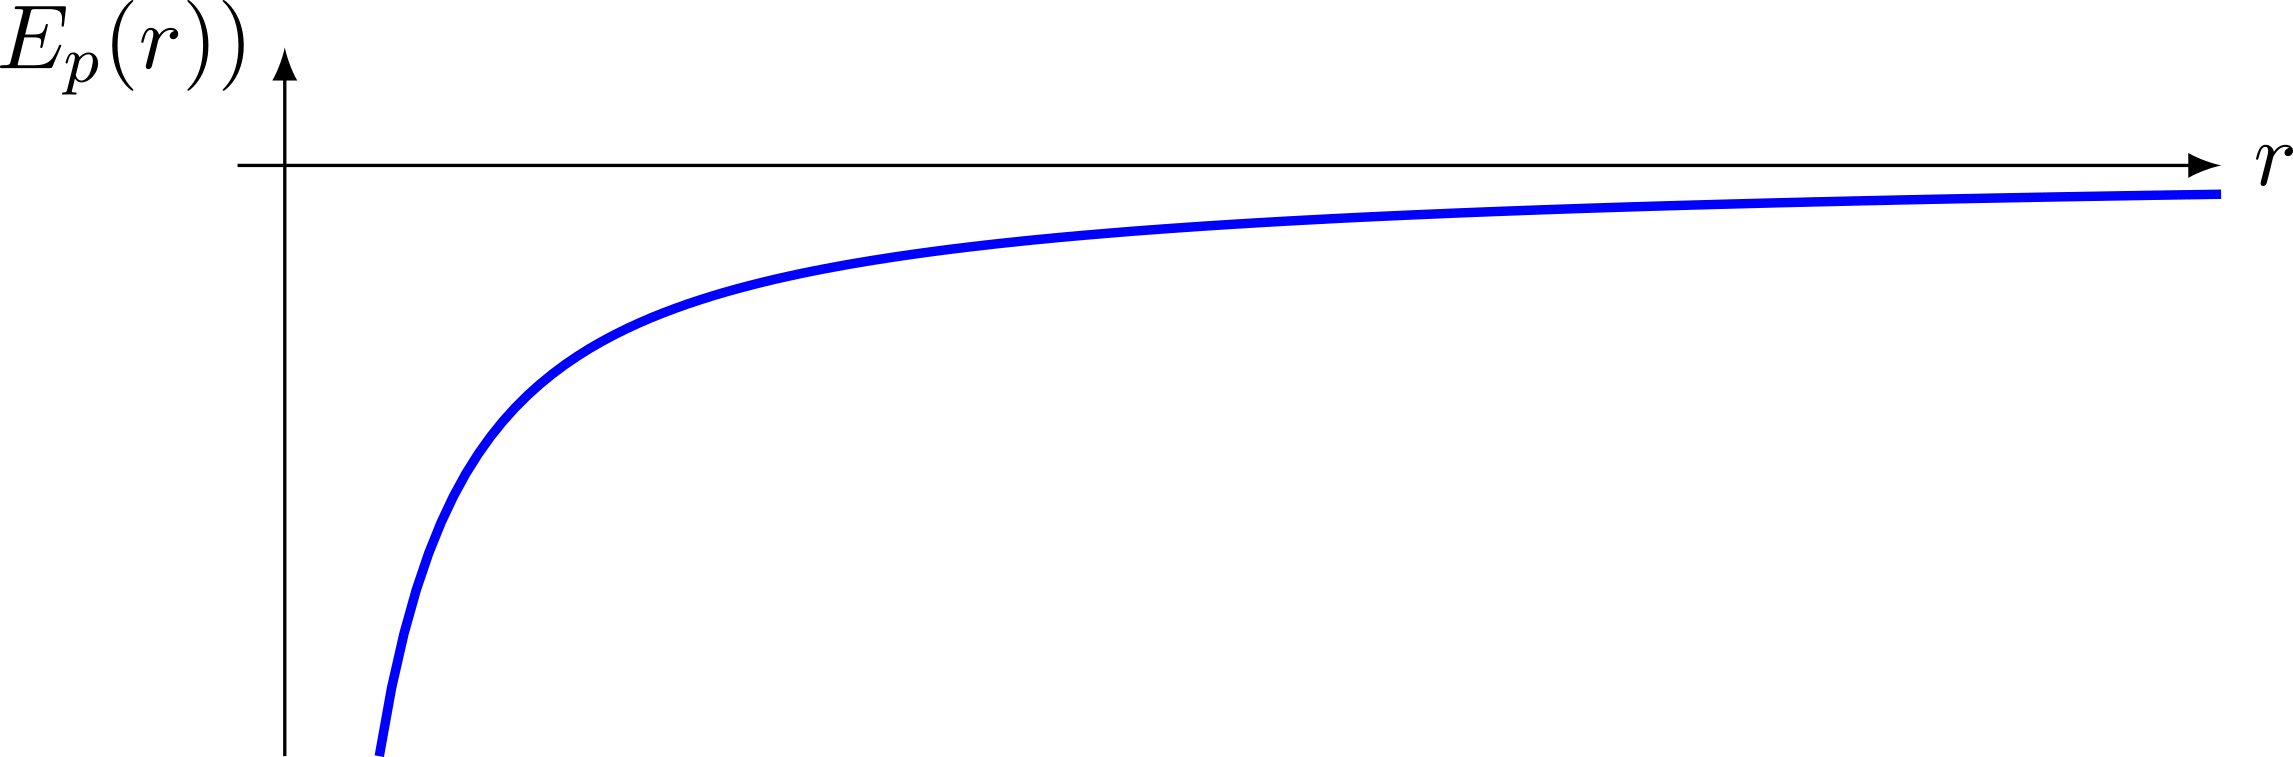
\includegraphics[width=\linewidth]{intro_ep-grav}
                \end{center}
            \end{minipage}
        \item Interaction électrostatique~: \smallbreak
            \begin{minipage}{0.45\linewidth}
                \begin{align*}
                    -\pdv{\Ec_p}{r} &= \frac{1}{4\pi\ep_0} \frac{qq_\Or}{r^2}
                    \\\Lra
                    \Aboxed{\Ec_p(r) &= \frac{1}{4\pi\ep_0} \frac{qq_\Or}{r}}
                \end{align*}
            \end{minipage}
            \hfill
            \begin{minipage}{0.45\linewidth}
                \begin{center}
                    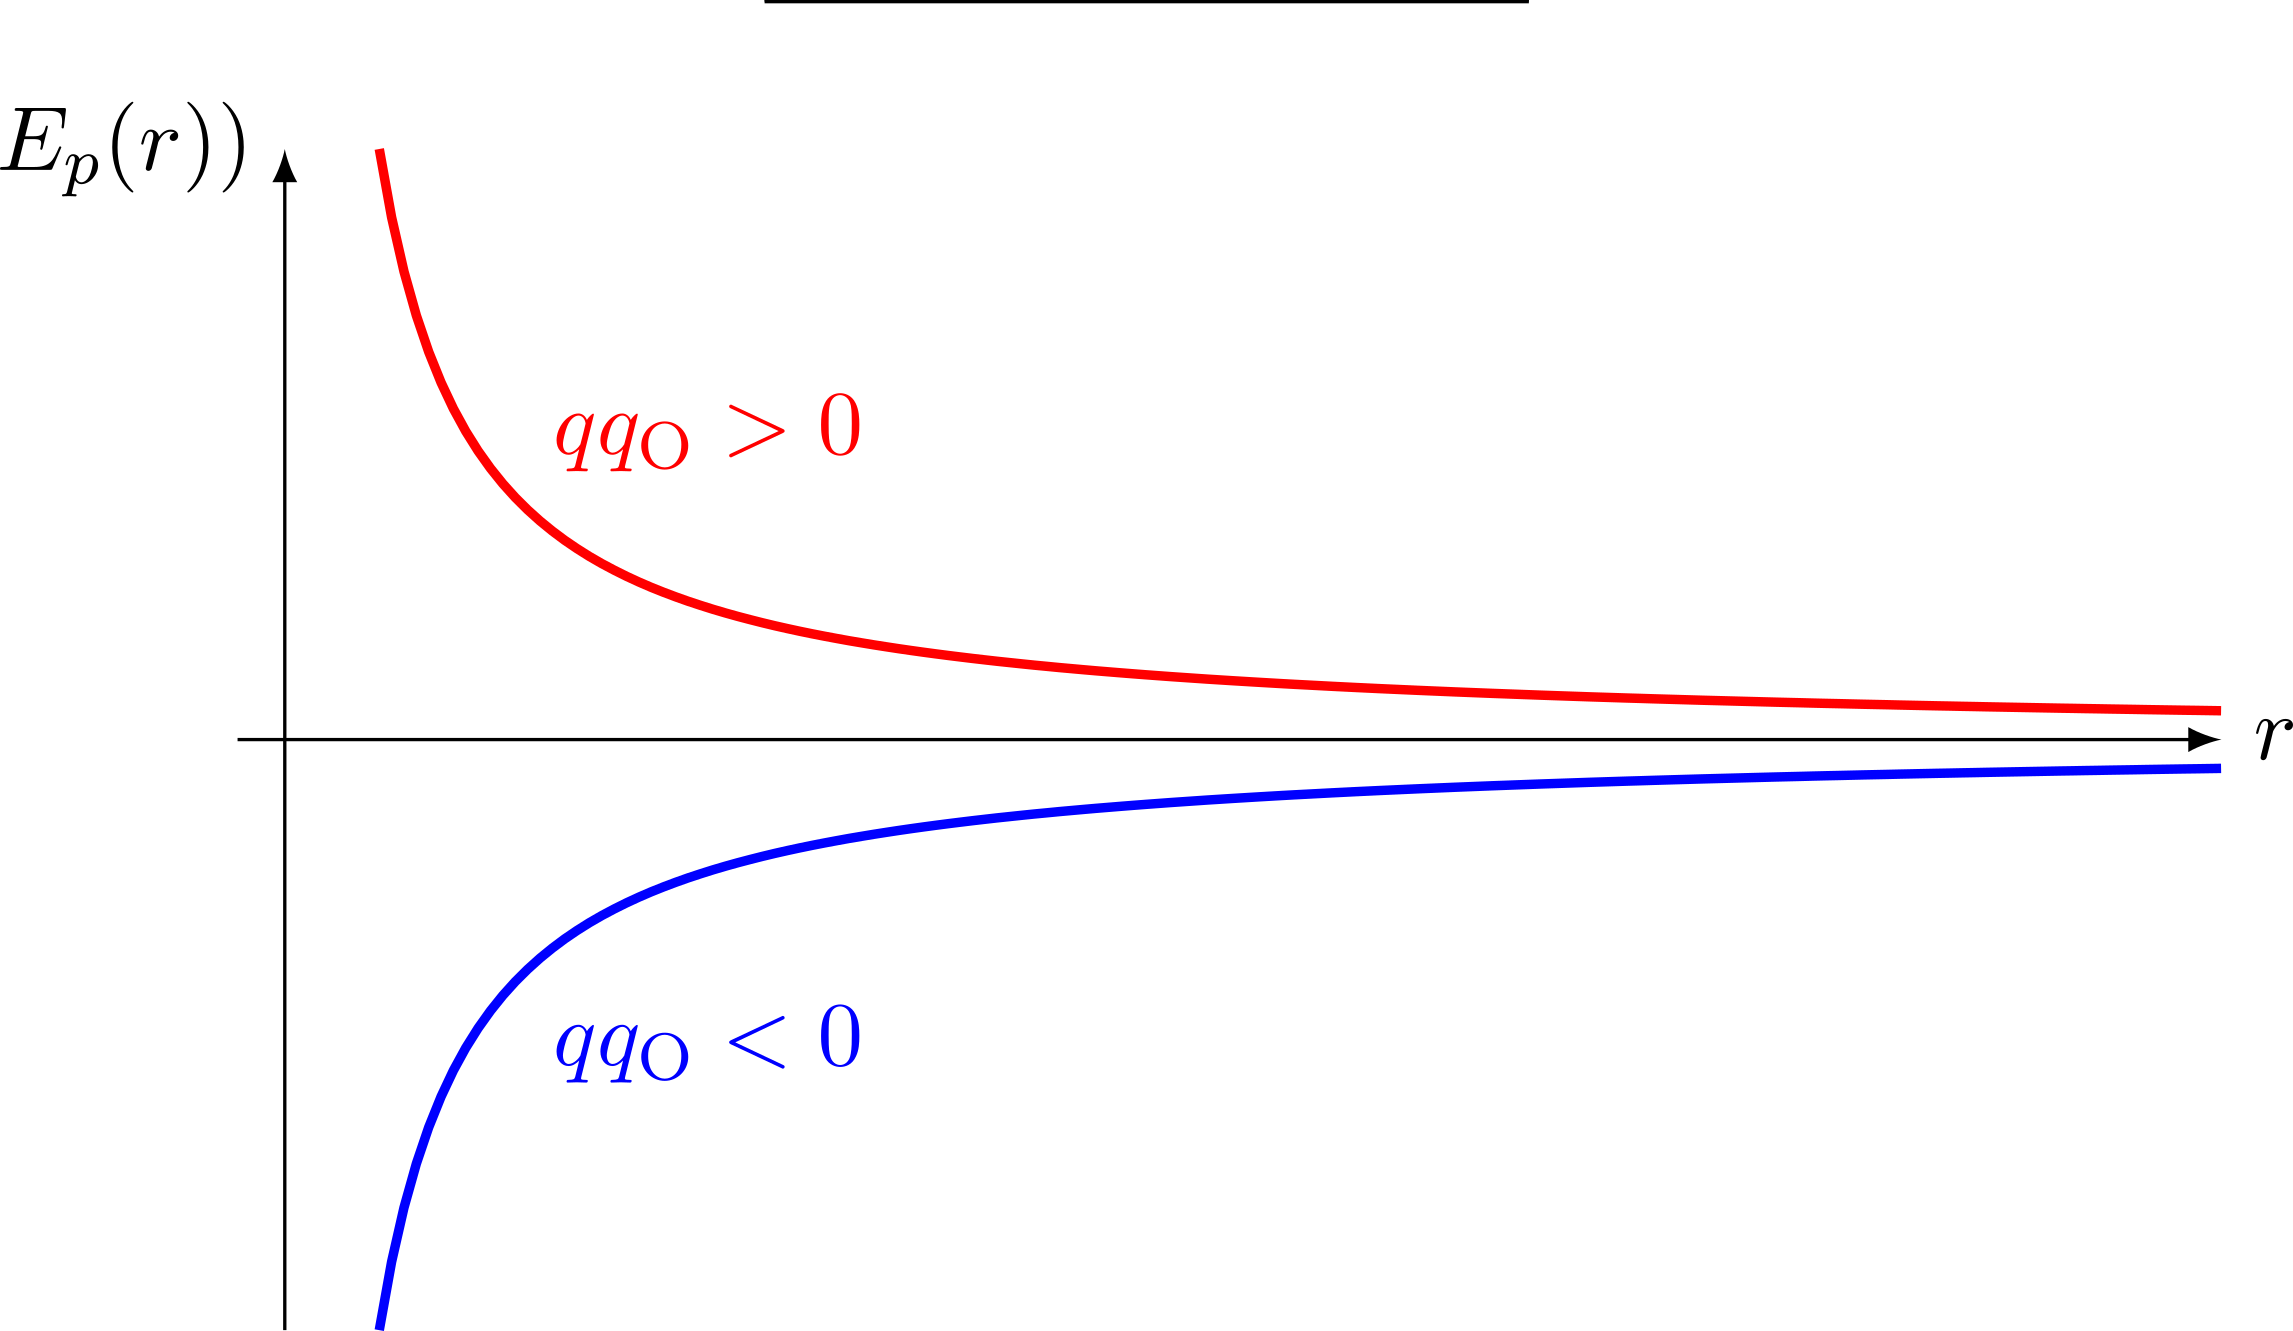
\includegraphics[width=\linewidth]{intro_ep-elec}
                \end{center}
            \end{minipage}
    \end{itemize}
\end{rexem}

\section{Quantités conservées}
\subsection{Conservation du moment cinétique}
On considère une force centrale $\Ff$ de centre O. Son moment par rapport à O
est
\[\Mcf_\Or(\Ff) = \OM\wedge\Ff = \of\]
Si M n'est soumis qu'à $\Ff$, le théorème du moment cinétique en O appliqué à M
donne
\[\dv{\Lcf_\Or}{t} = \Mcf_\Or(\Ff) = \of\]
Ainsi,
\begin{tprop}{Propriété~: conservation du moment cinétique, heart}
    Pour un point M soumis uniquement à $\Ff$ une force centrale, son moment
    cinétique par rapport au centre de force se conserve~:
    \[
        \boxed{
            \Lcf_\Or(\Mr) = \OM\wedge\pf = \vcte
            \Lra
            \dv{\Lcf_\Or}{t} = \Mcf_\Or(\Ff) = \of
        }
    \]
\end{tprop}
\textbf{Conséquence}~: Notons $\Lcf_0 = \Lc_0\uz$ le moment cinétique
initial, c'est-à-dire
\[\Lcf_0 = \OM(0)\wedge m\vf(0)\]
Si $\OM(0)$ et $\vf(O)$ ne sont pas colinéaires, alors $\uz$ définit une
direction perpendiculaire à $\OM(0)$ et $\vf(0)$, ici $\uz$. Or, comme $\Lcf$ se
conserve, on a
\[\Lcf(t) = \OM(t)\wedge m\vf(t) = \Lc_0\uz\]
donc $\OM$ et $\vf$ \textbf{restent orthogonaux} à $\uz$. Autrement dit,
\textbf{le mouvement reste dans le plan $\perp \uz$ passant par O}.
\begin{tcoro}{Conséquence de la conservation, heart}
    La conservation du moment cinétique d'un point matériel M par rapport à un
    point O fixe dans $\Rc$ implique que le mouvement \textbf{se fait dans le
    plan défini par} $\OM(0)$ et $\vf(0)$.
    \begin{center}
        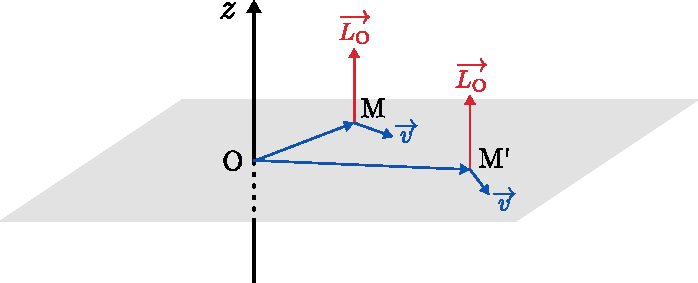
\includegraphics[width=.6\linewidth]{mvt_plan}
    \end{center}
\end{tcoro}

\begin{rrema}{Remarque}
    Si $\OM(0)$ et $\vf(0)$ sont colinéaires, alors $\Lcf_0$ est nul, et reste
    donc nul à tout instant~: $\OM$ et $\vf$ restent colinéaires, et le
    mouvement est alors simplement rectiligne.
\end{rrema}

\subsection{Loi des aires}
\subsubsection{Deuxième loi de \textsc{Kepler}}

\begin{tprop}{Aire d'un triangle, hand}
    \begin{minipage}{0.80\linewidth}
        L'aire d'un triangle ABC peut être calculée à partir de la formule~:
        \[\Ac = \frac{1}{2}\norm{\AB\wedge\vv{\rm AC}}\]
    \end{minipage}
    \hfill
    \begin{minipage}{0.19\linewidth}
        \begin{center}
            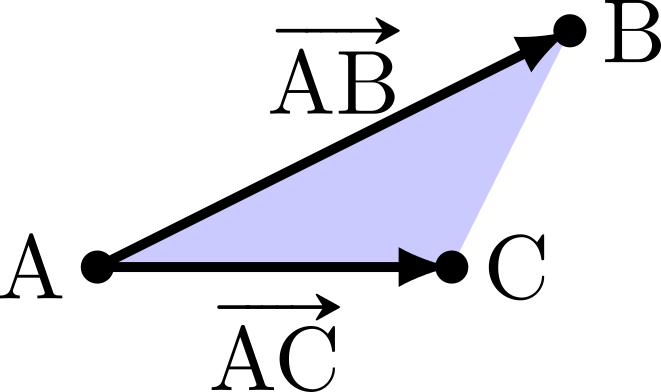
\includegraphics[scale=1]{aire_tri}
        \end{center}
    \end{minipage}
\end{tprop}
Ainsi, en prenant M comme origine du repère et correspondant à A dans la formule
proposée, on peut déterminer l'aire dite «~balayée~» par le point M autour de O
pendant un temps $\dt$, tel que le mouvement soit suffisamment court pour
décrire le triangle OM$(t)$M$(t+\dt)$~:
\begin{align*}
    \dd{\Ac} &= \frac{1}{2}\norm{\vv{\Mr(t)\Or}\wedge\vv{\Mr(t)\Mr(t+\dt)}}
    \shortintertext{Or, par construction on a $\vv{\Mr(t)\Mr(t+\dt)} = \vf\dt$,
    d'où}
    \dd{\Ac} &= \frac{1}{2}\norm{-\OM(t)\wedge\vf}\dt
    \\\Lra
    \Aboxed{\dv{\Ac}{t} &= \frac{\norm{\Lcf_\Or}}{2m} = \cte}
\end{align*}
ce qui est la deuxième loi de \textsc{Kepler}, dont on rediscutera plus tard~:
\begin{tprop}{Deuxième loi de \textsc{Kepler}, heart}
    \begin{minipage}{0.44\linewidth}
        Pour un point M soumis uniquement à une force centrale, des aires égales
        sont balayées pendant un temps égal.
    \end{minipage}
    \hfill
    \begin{minipage}{0.55\linewidth}
        \begin{center}
            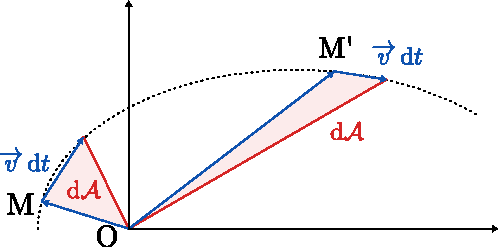
\includegraphics[scale=1]{kepler_2-aire}
        \end{center}
    \end{minipage}
\end{tprop}

\subsubsection{Constante des aires}
On se rend alors compte qu'une quantité constante intervient régulièrement dans
l'étude des mouvements à force centrale. Reprenons les coordonnées cylindriques
centrées sur O, avec $\uz \perp \Lcf_0$ donc perpendiculaire au mouvement. On a
\begin{align*}
    \OM &= r\ur
    \\\Ra
    \vf &= \rp\ur + r\tp\ut
    \\\Ra
    \Lcf_\Or &= \OM\wedge m\vf = mr^2\tp
\end{align*}
Ainsi,
\begin{tdefi}{Constante des aires, heart}
    La \textbf{constante des aires} est la grandeur
    \[C = r^2\tp\]
    et est une quantité constante au cours du mouvement. Notamment, $\tp$ est de
    \textbf{signe constant}, et la rotation se fait toujours dans le même sens.
\end{tdefi}

\subsection{Conservation de l'énergie mécanique}
Toujours pour M soumis uniquement à une force centrale conservative.
On a
\begin{align*}
    \Ec_m &= \Ec_c + \Ec_p
    \shortintertext{et d'après le TEM, $\Ec_m$ est constante. De plus,}
    v^2 &= \rp^2 + (r\tp)^2
    \\\Ra
    \Ec_m &= \frac{1}{2}m\rp^2 + \frac{1}{2}mr^2\tp^2 + \Ec_p
    \shortintertext{et avec $\tp = C/r^2$~:}
    \Ec_m &= \frac{1}{2}m\rp^2 + \frac{1}{2}m \frac{C^2}{r^2} + \Ec_p
\end{align*}
\begin{tdefi}{Définition~: énergie potentielle effective, hand}
    On appelle \textbf{énergie potentielle effective} et on note $\Ec_{p,\rm
    eff}$ la grandeur
    \[\boxed{\Ec_{p,\rm eff} = \frac{1}{2}m \frac{C^2}{r^2} + \Ec_p}\]
\end{tdefi}
L'énergie potentielle effective permet de se ramener à l'étude d'une seule
dimension, ici $r$ la distance au centre de force, plutôt que d'utiliser à la
fois $r$ et $\tt$, en considérant $\Ec_{p,\rm eff}$ comme l'énergie potentielle
du système.

\section{Champs de force newtoniens}
\subsection{Définition}
\begin{tdefi}{Définition, sidebyside}
    Une force centrale est dite \textbf{newtonienne} si elle s'exprime sous la
    forme
    \[\boxed{\Ff = -\frac{k}{r^2}\ur}\]
    Si $k>0$, la force est attractive~; si $k<0$, elle est répulsive.
    \tcblower
    L'énergie potentielle associée est alors
    \[\boxed{\Ec_p(r) = -\frac{k}{r}}\]
\end{tdefi}
\begin{rexem}{Exemples}
    \begin{itemize}
        \item Pour l'interaction gravitationnelle, $k = \Gc m_\Or m$~;
        \item Pour l'interaction électrostatique, $k = -q_\Or q/4\pi\ep_0$.
    \end{itemize}
\end{rexem}

Ainsi, l'énergie potentielle \textbf{effective} pour un système à force centrale
conservative newtonienne est
\[\boxed{\Ec_{p,\rm eff} = \frac{1}{2}m\frac{C^2}{r^2} - \frac{k}{r}}\]
Nous allons maintenant étudier les différentes trajectoires possibles en
fonction de l'énergie mécanique totale et de cette énergie potentielle
effective.

\subsection{Cas attractif}
\subsubsection{Étude mathématique}
Analysons la fonction $\Ec_{p,\rm eff}(r)$~:
\begin{itemize}[label=$\diamond$]
    \item $\DS \lim_{r\to0} \Ec_{p,\rm eff}(r) = +\infty$~;
    \item $\DS \lim_{r\to+\infty} \Ec_{p,\rm eff}(r) = 0$~;
    \item $\Ec_{p,\rm eff}$ présente un minimum. En effet, \smallbreak
        \begin{minipage}{0.45\linewidth}
            \begin{align*}
                \dv{\Ec_{p,\rm eff}}{r} &= 0
                \\\Lra
                \frac{1}{2}m\left(-2 \frac{C^2}{r^3}\right) + \frac{k}{r^2} &= 0
                \\\Lra
                -mC^2 + kr &= 0
                \\\Lra
                \Aboxed{r_{\min} &= \frac{mC^2}{k}}
                \shortintertext{et alors}
                \Ec_{p,\rm eff}(r_{\min}) &= -\frac{k^2}{2mC^2}
            \end{align*}
        \end{minipage}
        \hfill
        \begin{minipage}{0.50\linewidth}
            \begin{center}
                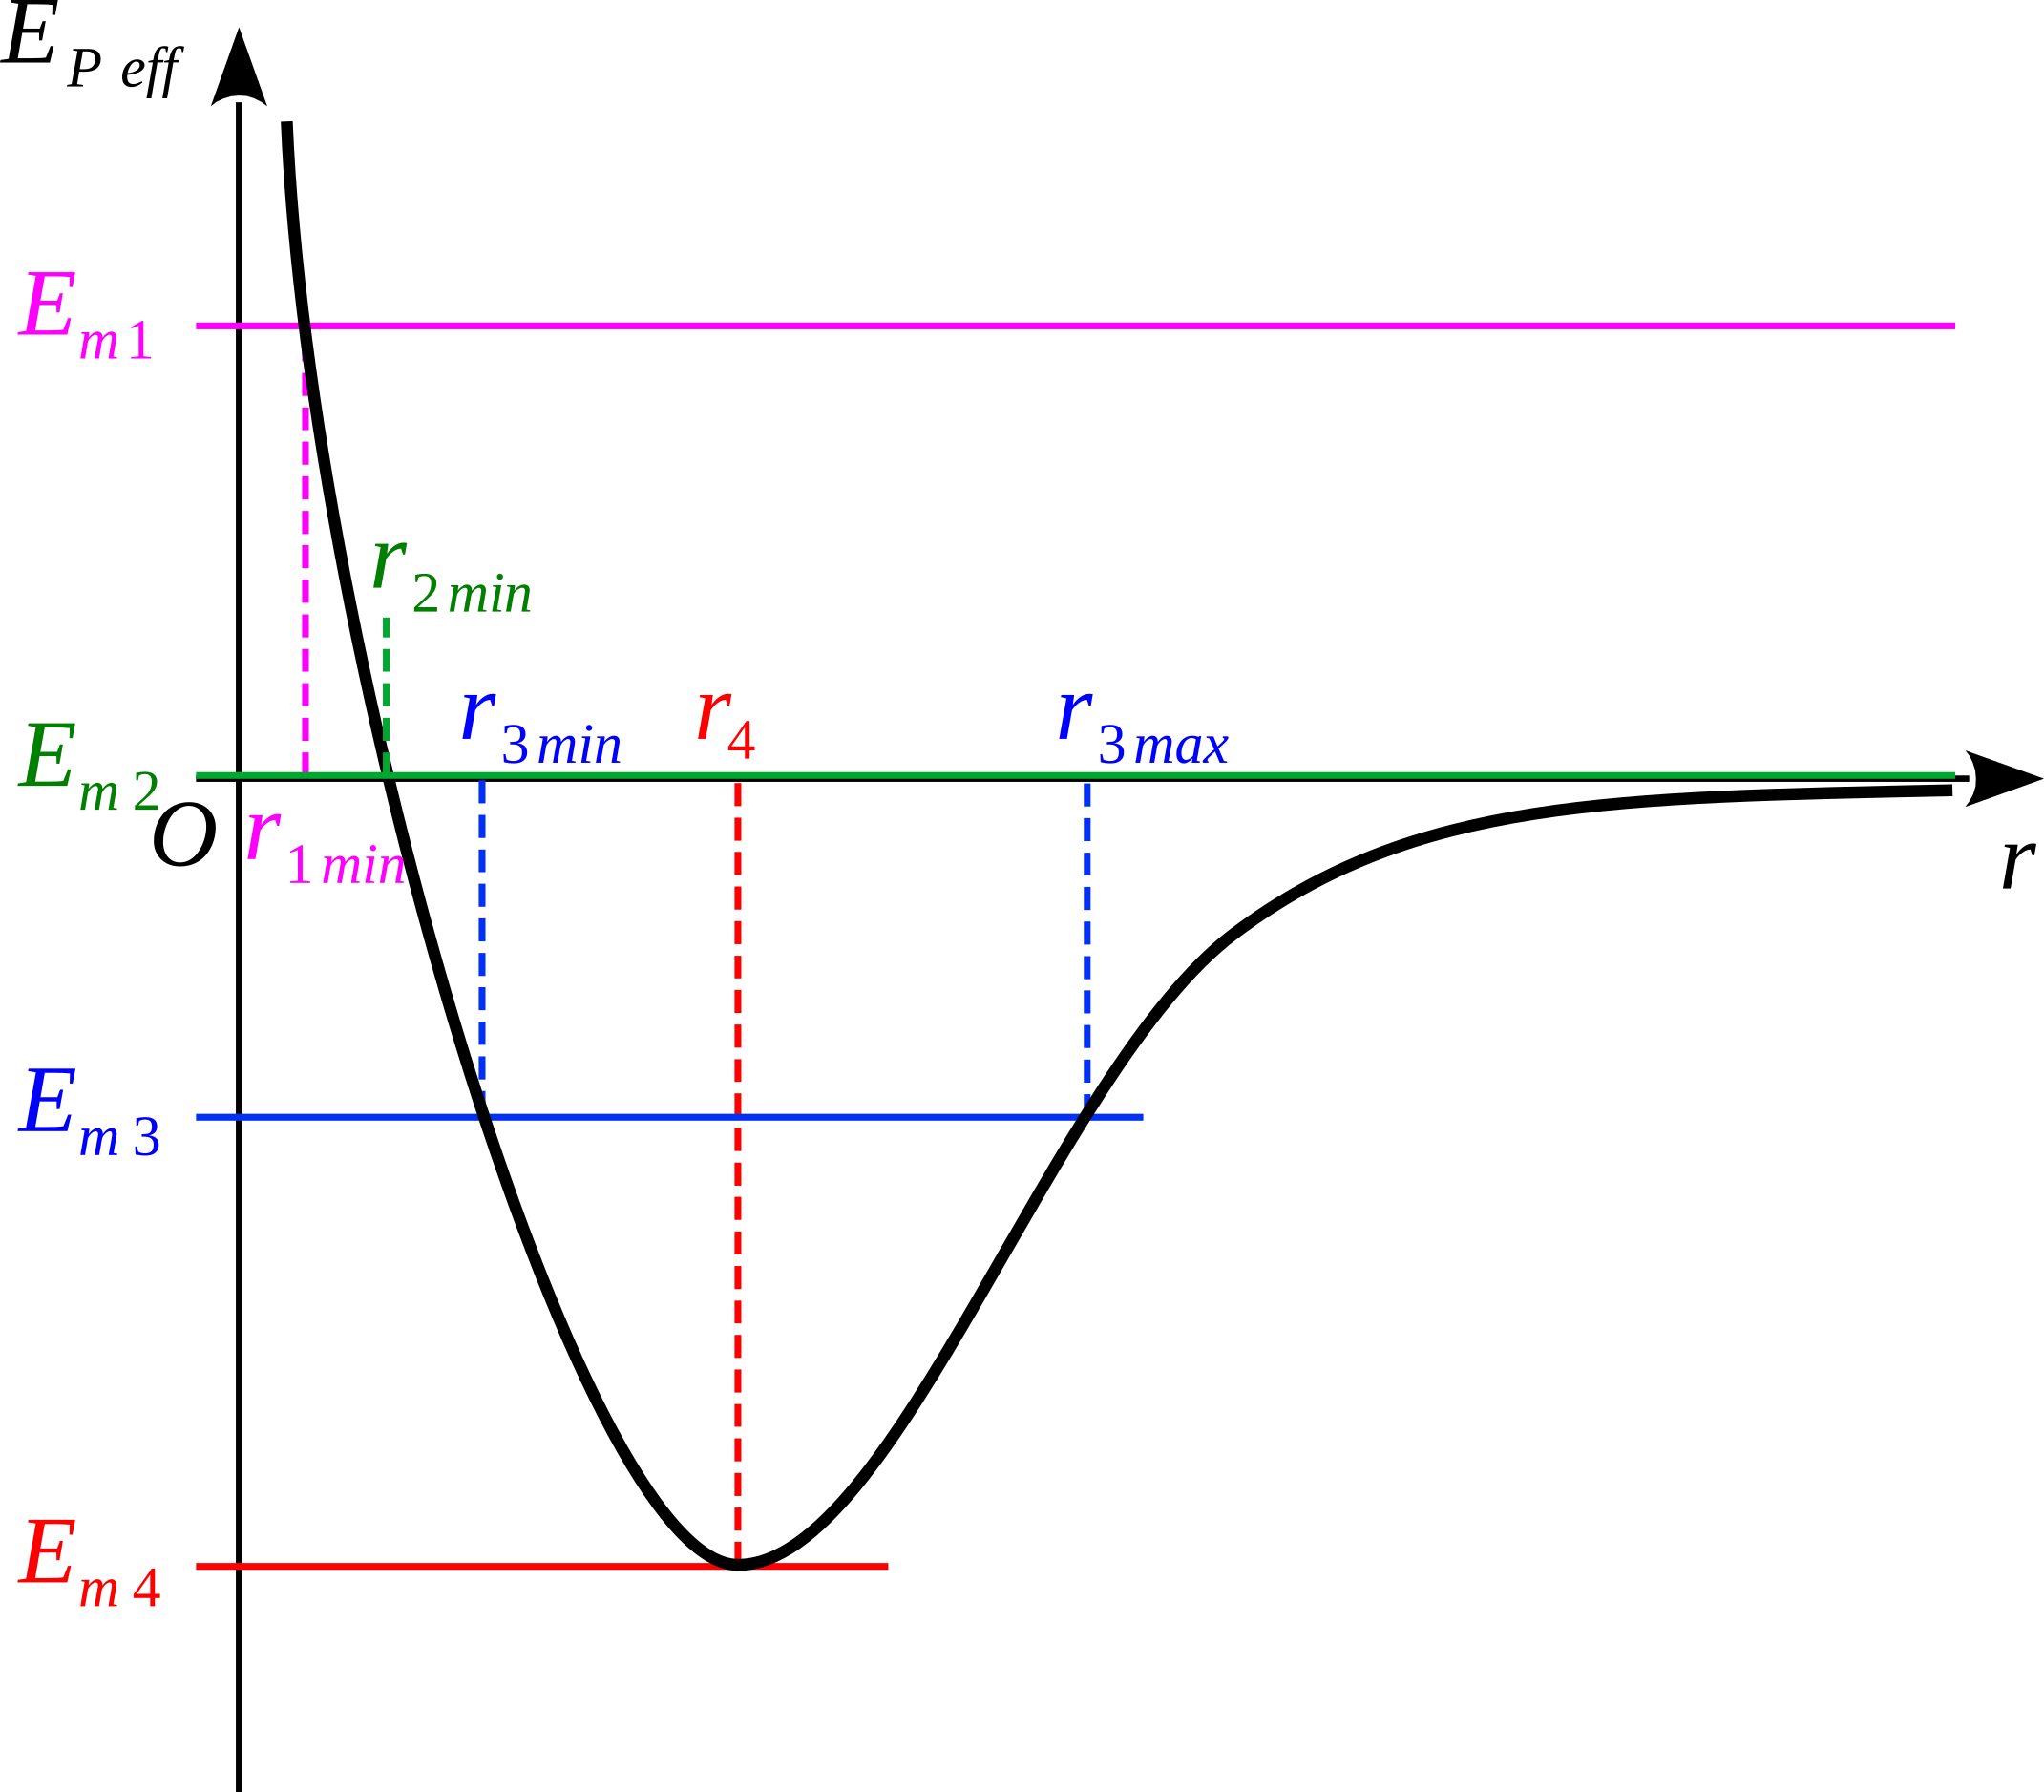
\includegraphics[width=\linewidth]{ep_eff-att_color}
            \end{center}
        \end{minipage} \smallbreak
        que l'on notera $-U_0$ ou $-\Ec_0$.
\end{itemize}

\subsubsection{Étude des trajectoires}
Comme $\Ec_m = \frac{1}{2}m\rp^2 + \Ec_{p,\rm eff}$, $\Ec_{p,\rm eff} < \Ec_m$.
Ainsi, selon la valeur de $\Ec_m$ par rapport à $\Ec_{p,\rm eff}(r)$, le système
aura différentes trajectoires, toutes ayant O comme foyer ou centre~:
\begin{itemize}
    \item Pour $\Ec_m \geq 0$, la trajectoire n'est \textbf{pas bornée}, on aura
        donc un état de \textbf{diffusion} avec deux valeurs minimales possibles
        et deux trajectoires possibles, hyperbolique et parabolique~;
    \item Pour $\Ec_m < 0$, la trajectoire \textbf{est bornée}, on aura donc un
        état \textbf{lié} avec deux valeurs extrêmes différentes pour la
        trajectoire elliptique ou une seule, $r_{\min}$, pour la trajectoire
        circulaire.
\end{itemize}

% \begin{table}[h]
%     \begin{tabularx}{\linewidth}{lYY}
%         \toprule
%         \multirow{2}{*}[-3pt]{Caractéristique} &
%         \multicolumn{2}{c}{Type de mouvement}
%         \\\cmidrule(lr){2-3}
%         &
%         \textbf{Diffusion} $\Ec_m \geq 0$
%         &
%         \textbf{Lié} $\Ec_m < 0$
%         \\\midrule
%         Valeur de $\Ec_m$ &
%         $0 < \Ec_m < \infty$ &
%         $-\Ec_0 < \Ec_m < 0$
%         \\
%         Graphique &
%         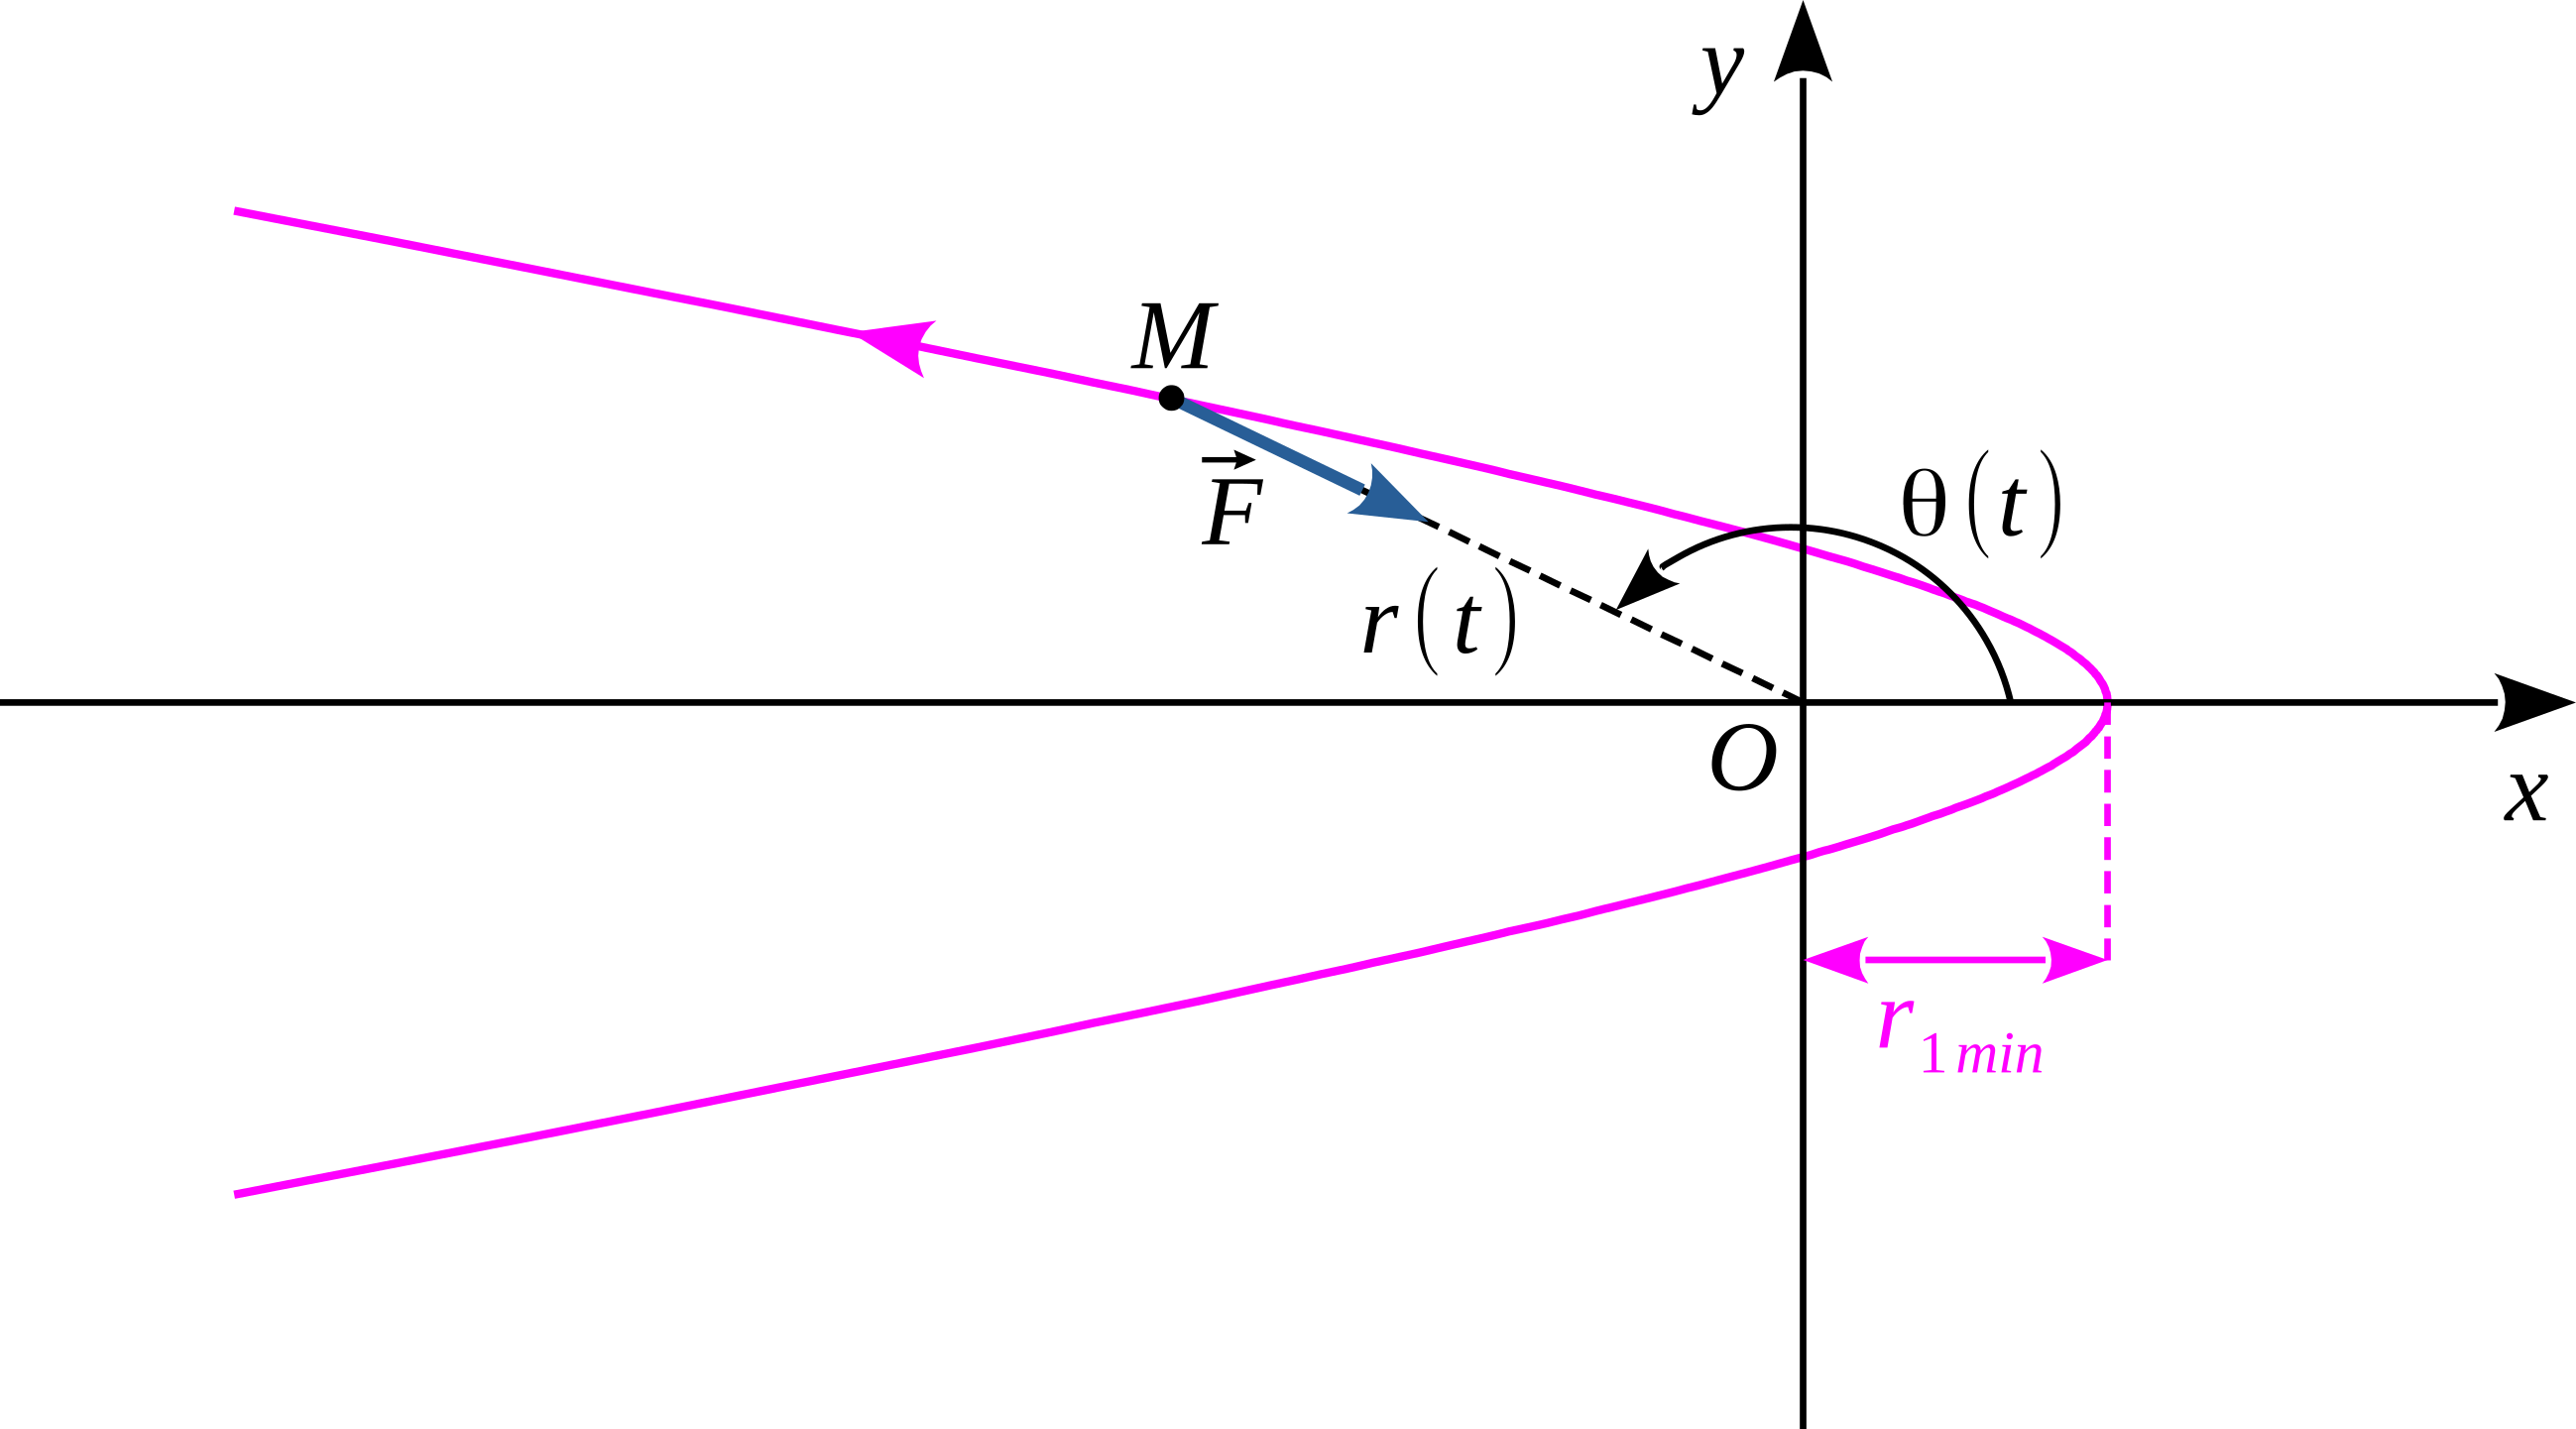
\includegraphics[width=\linewidth]{traj_att-color_hyp} &
%         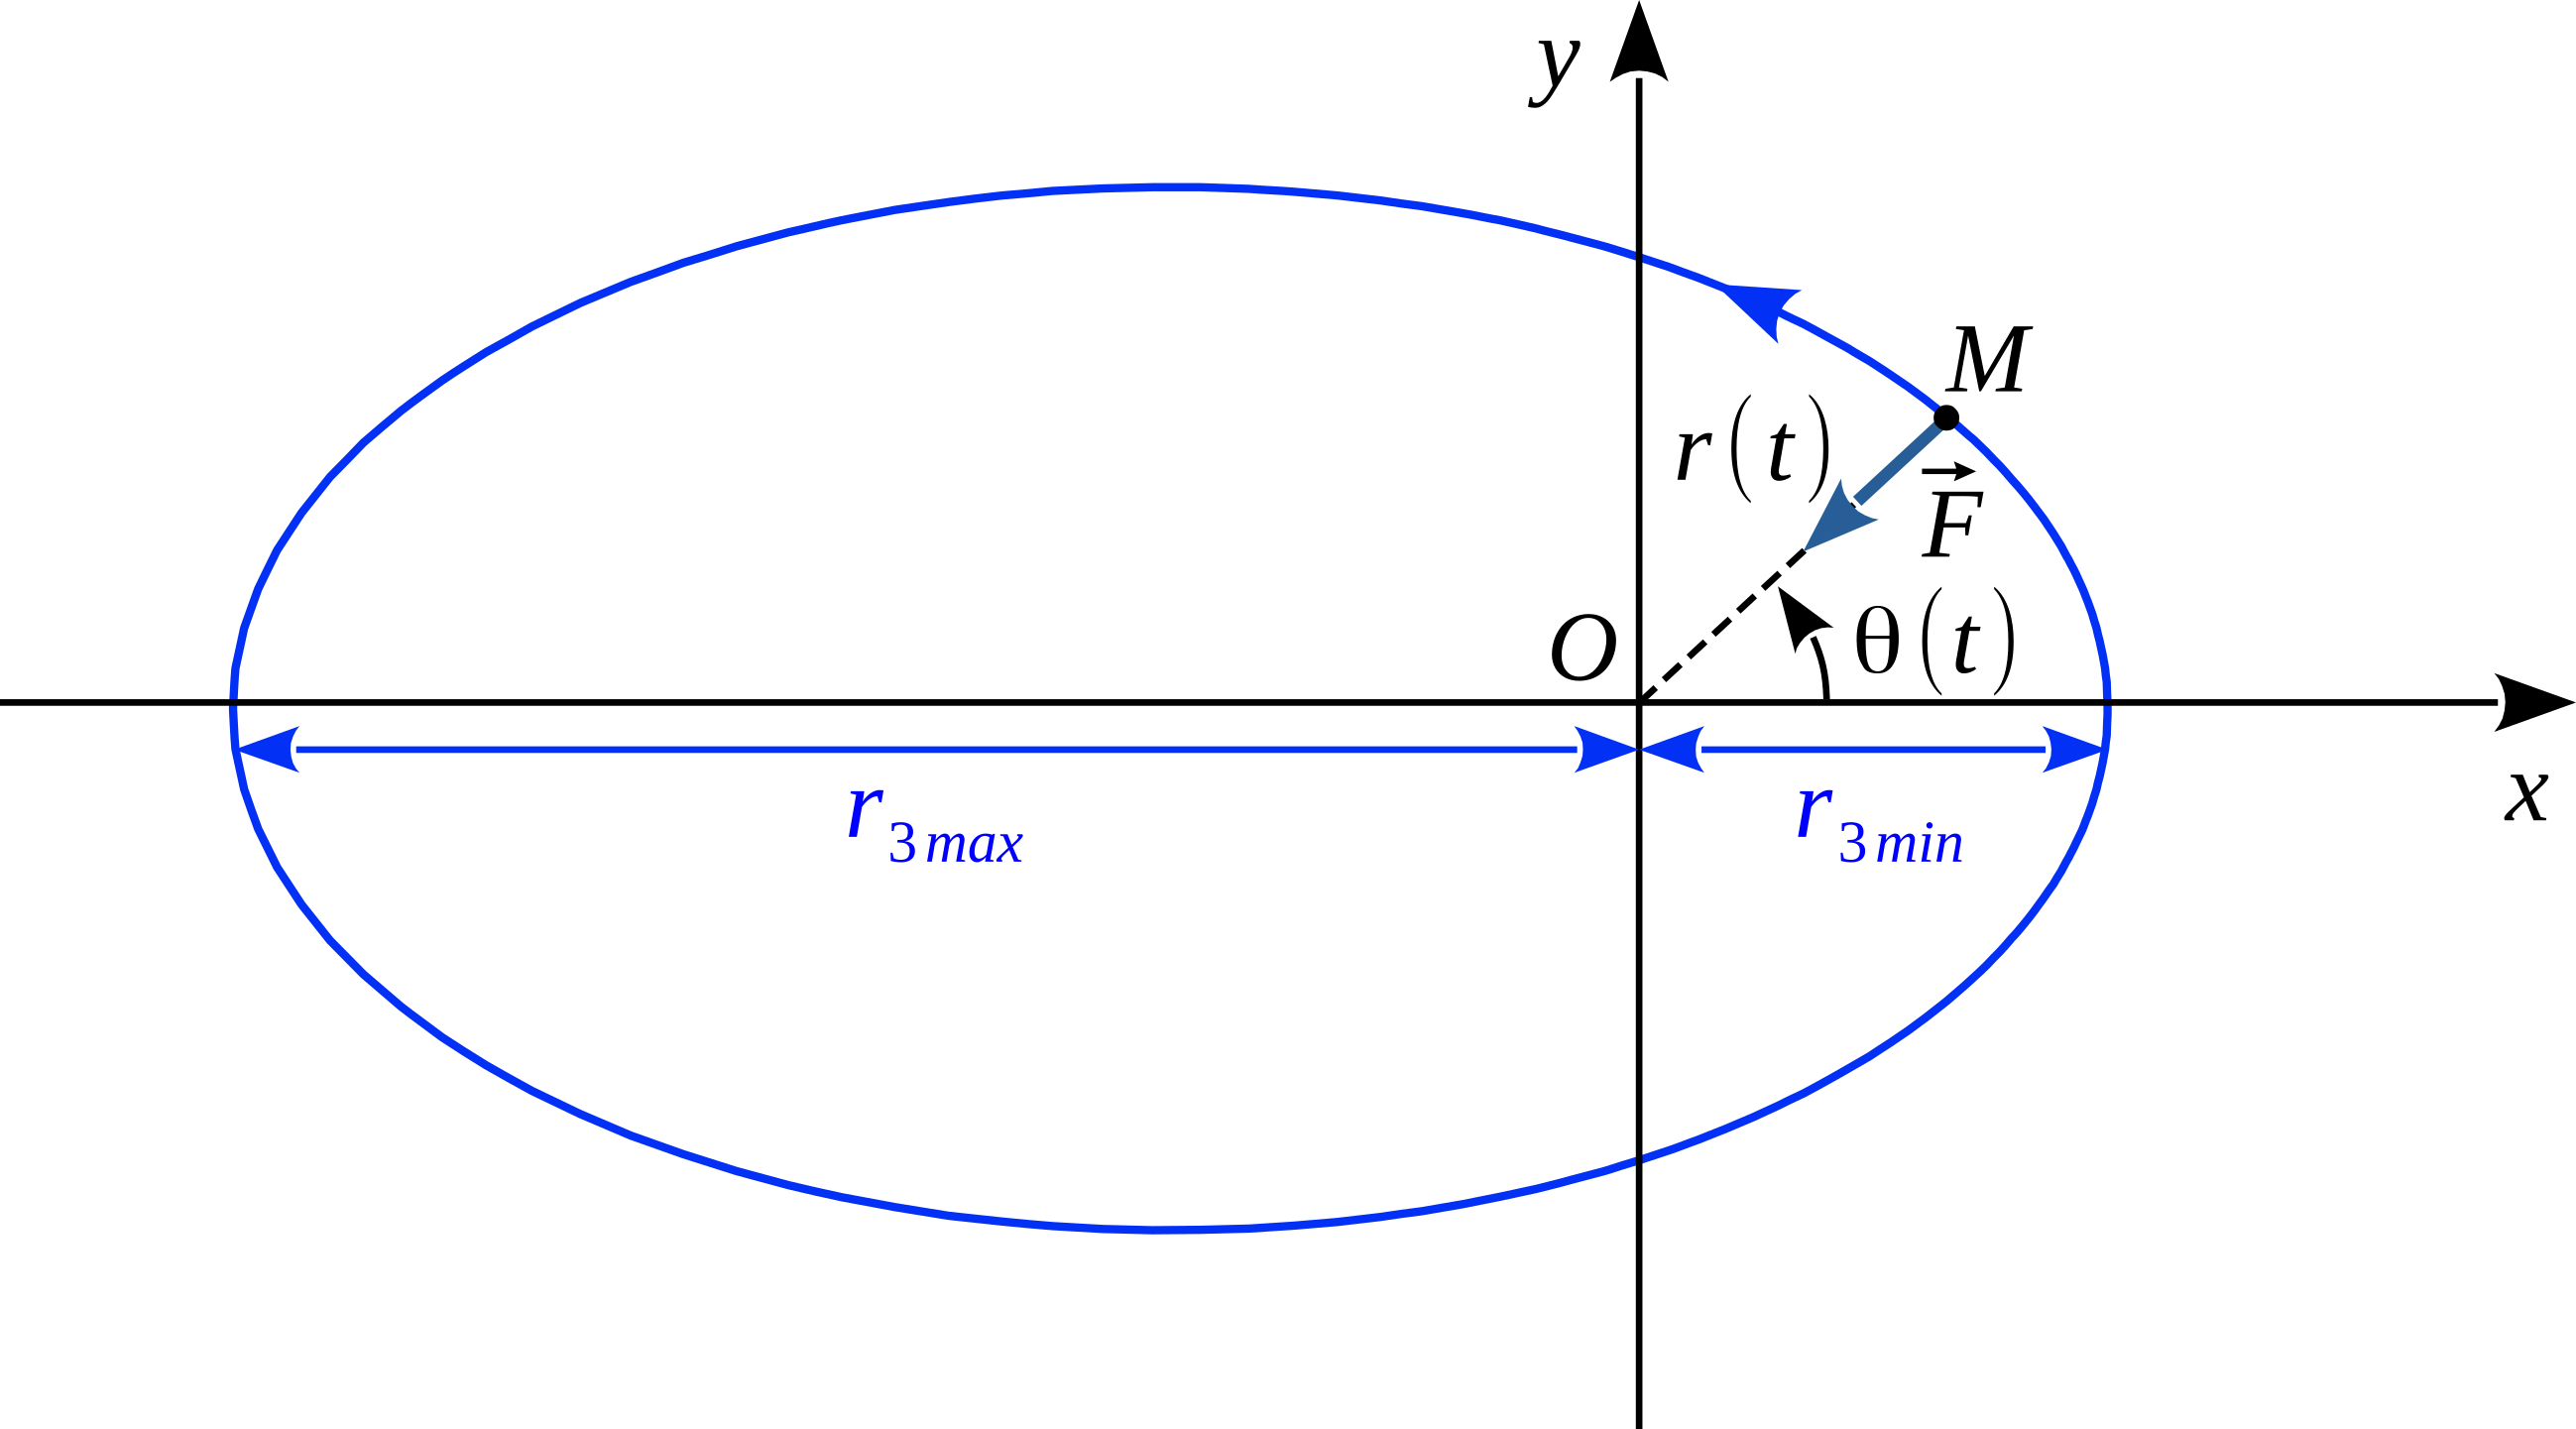
\includegraphics[width=\linewidth]{traj_att-color_ell}
%         \\
%         Trajectoire &
%         \textbf{hyperbolique} &
%         \textbf{elliptique}
%         \\\midrule
%         Valeur de $\Ec_m$ &
%         $\Ec_m = 0$ &
%         $0 < \Ec_m < \infty$
%         \\
%         Graphique &
%         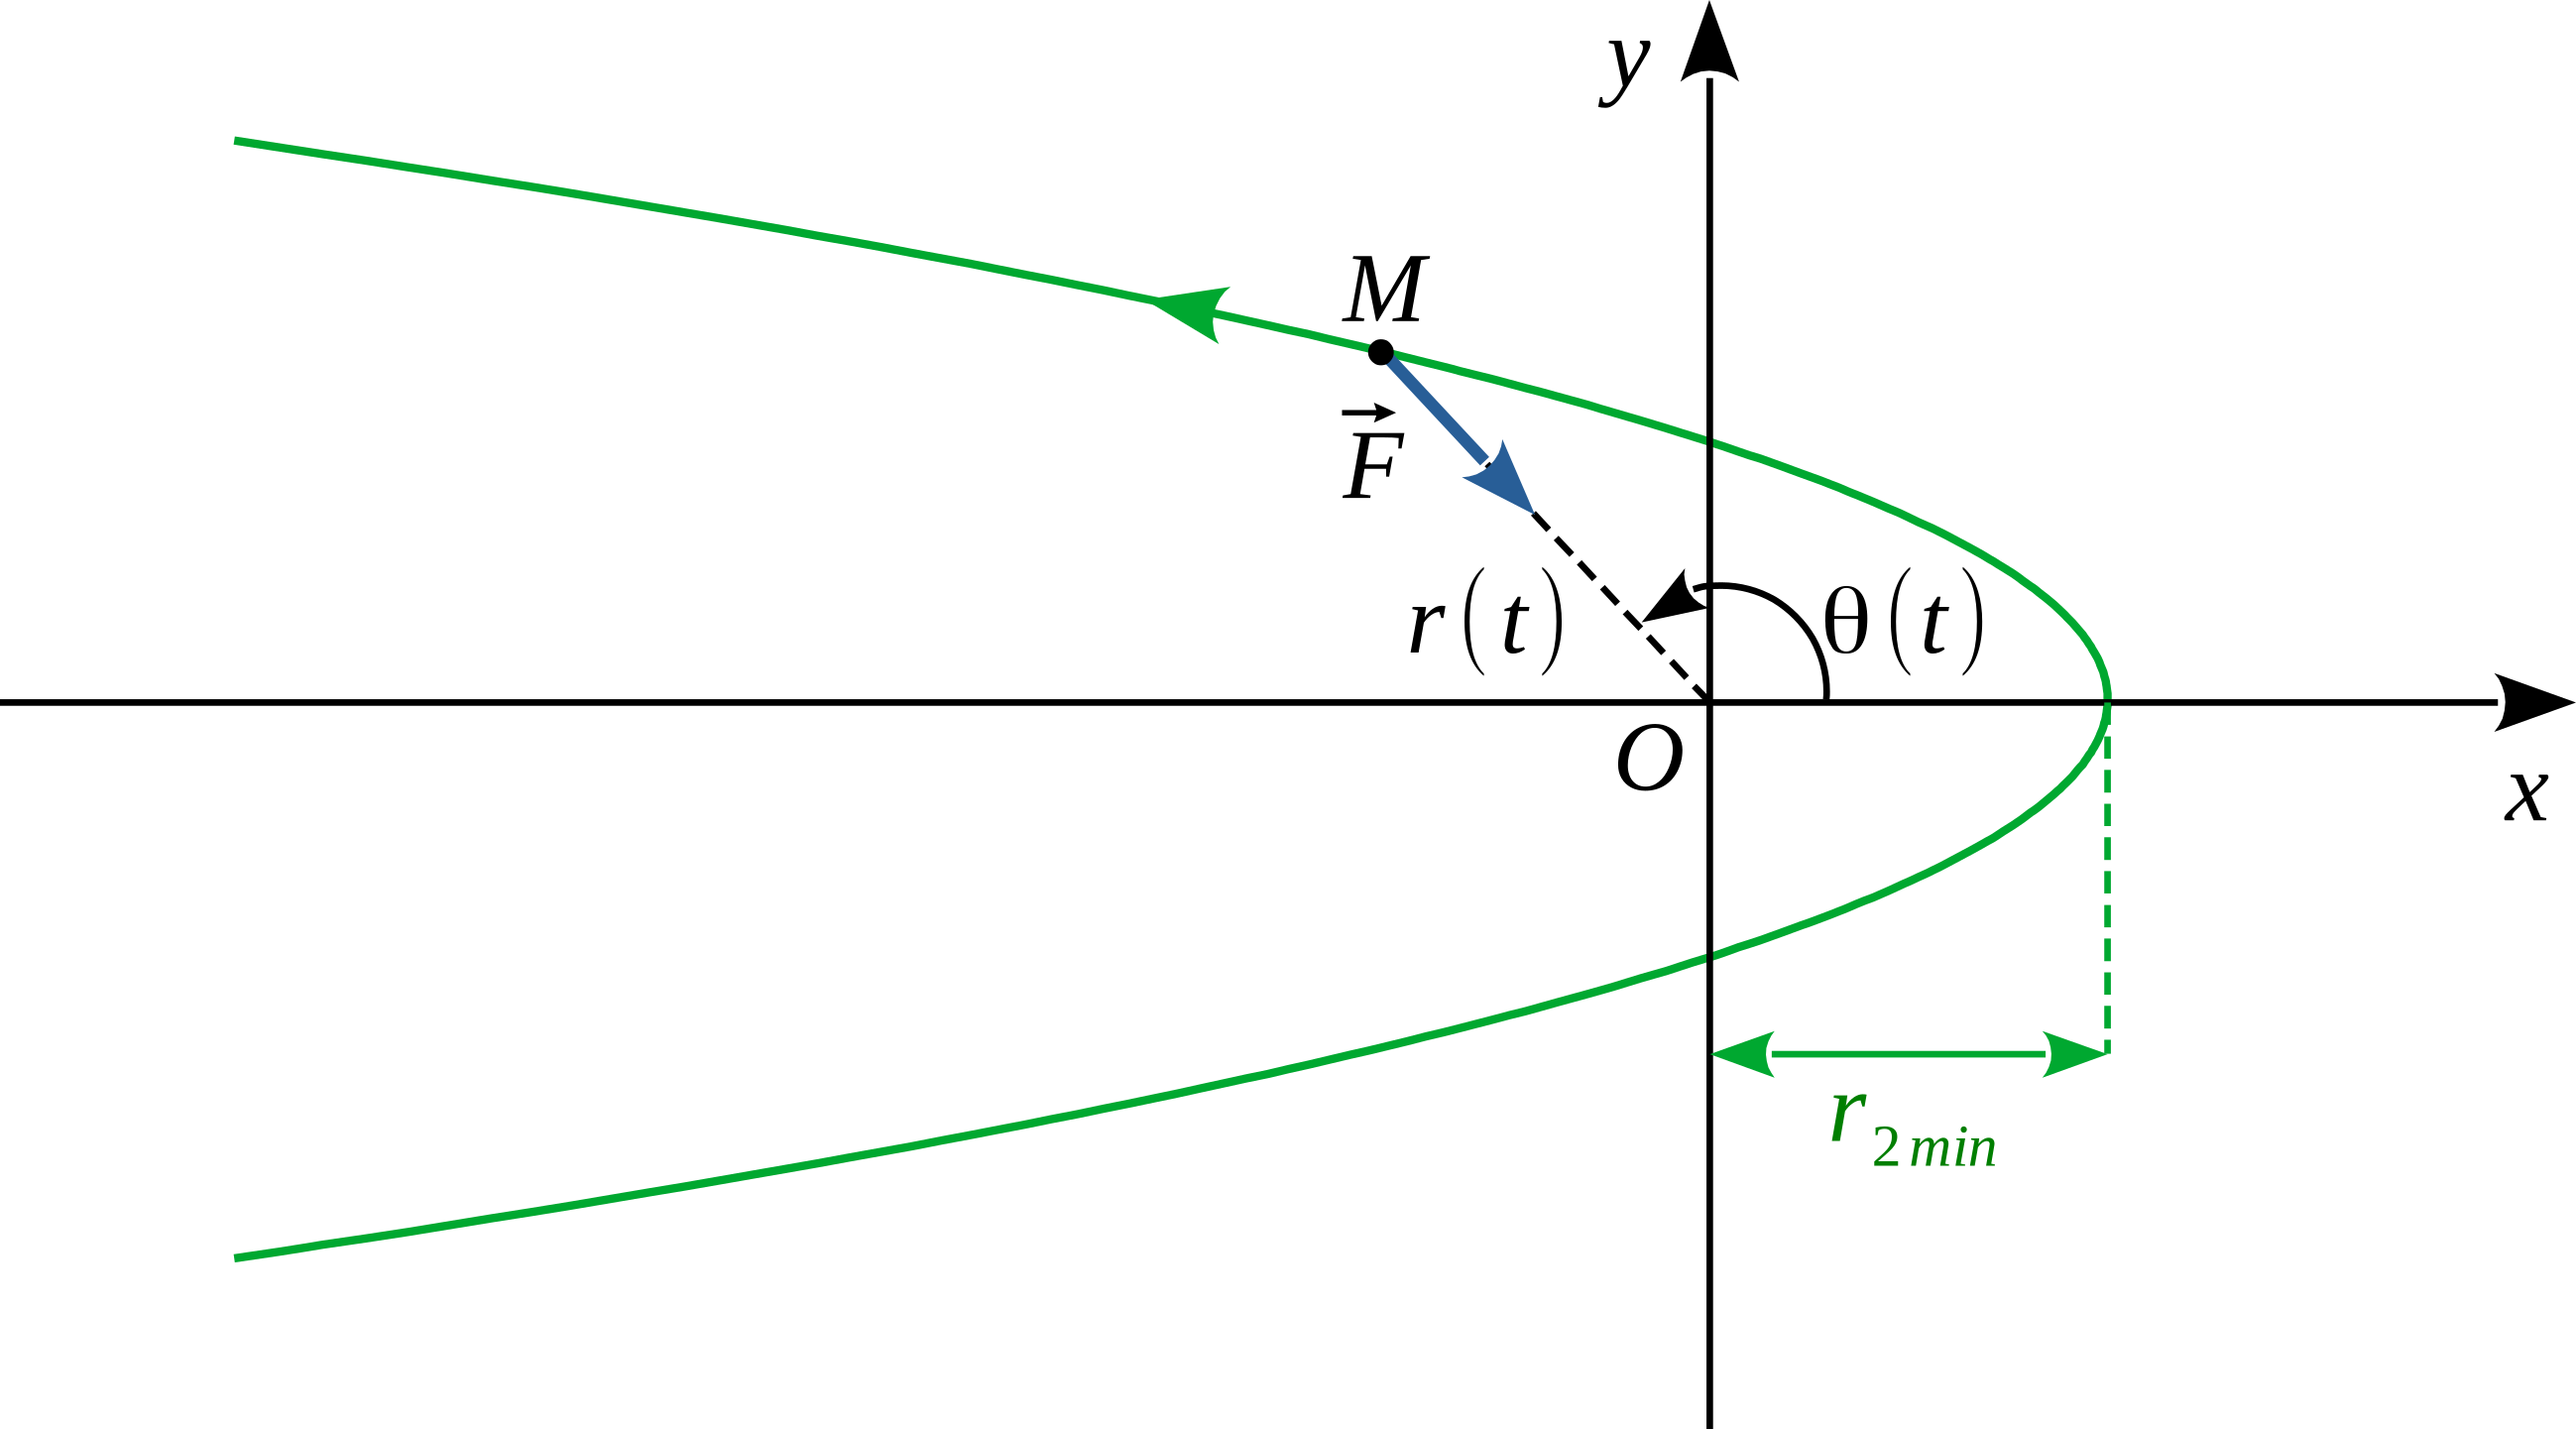
\includegraphics[width=\linewidth]{traj_att-color_par} &
%         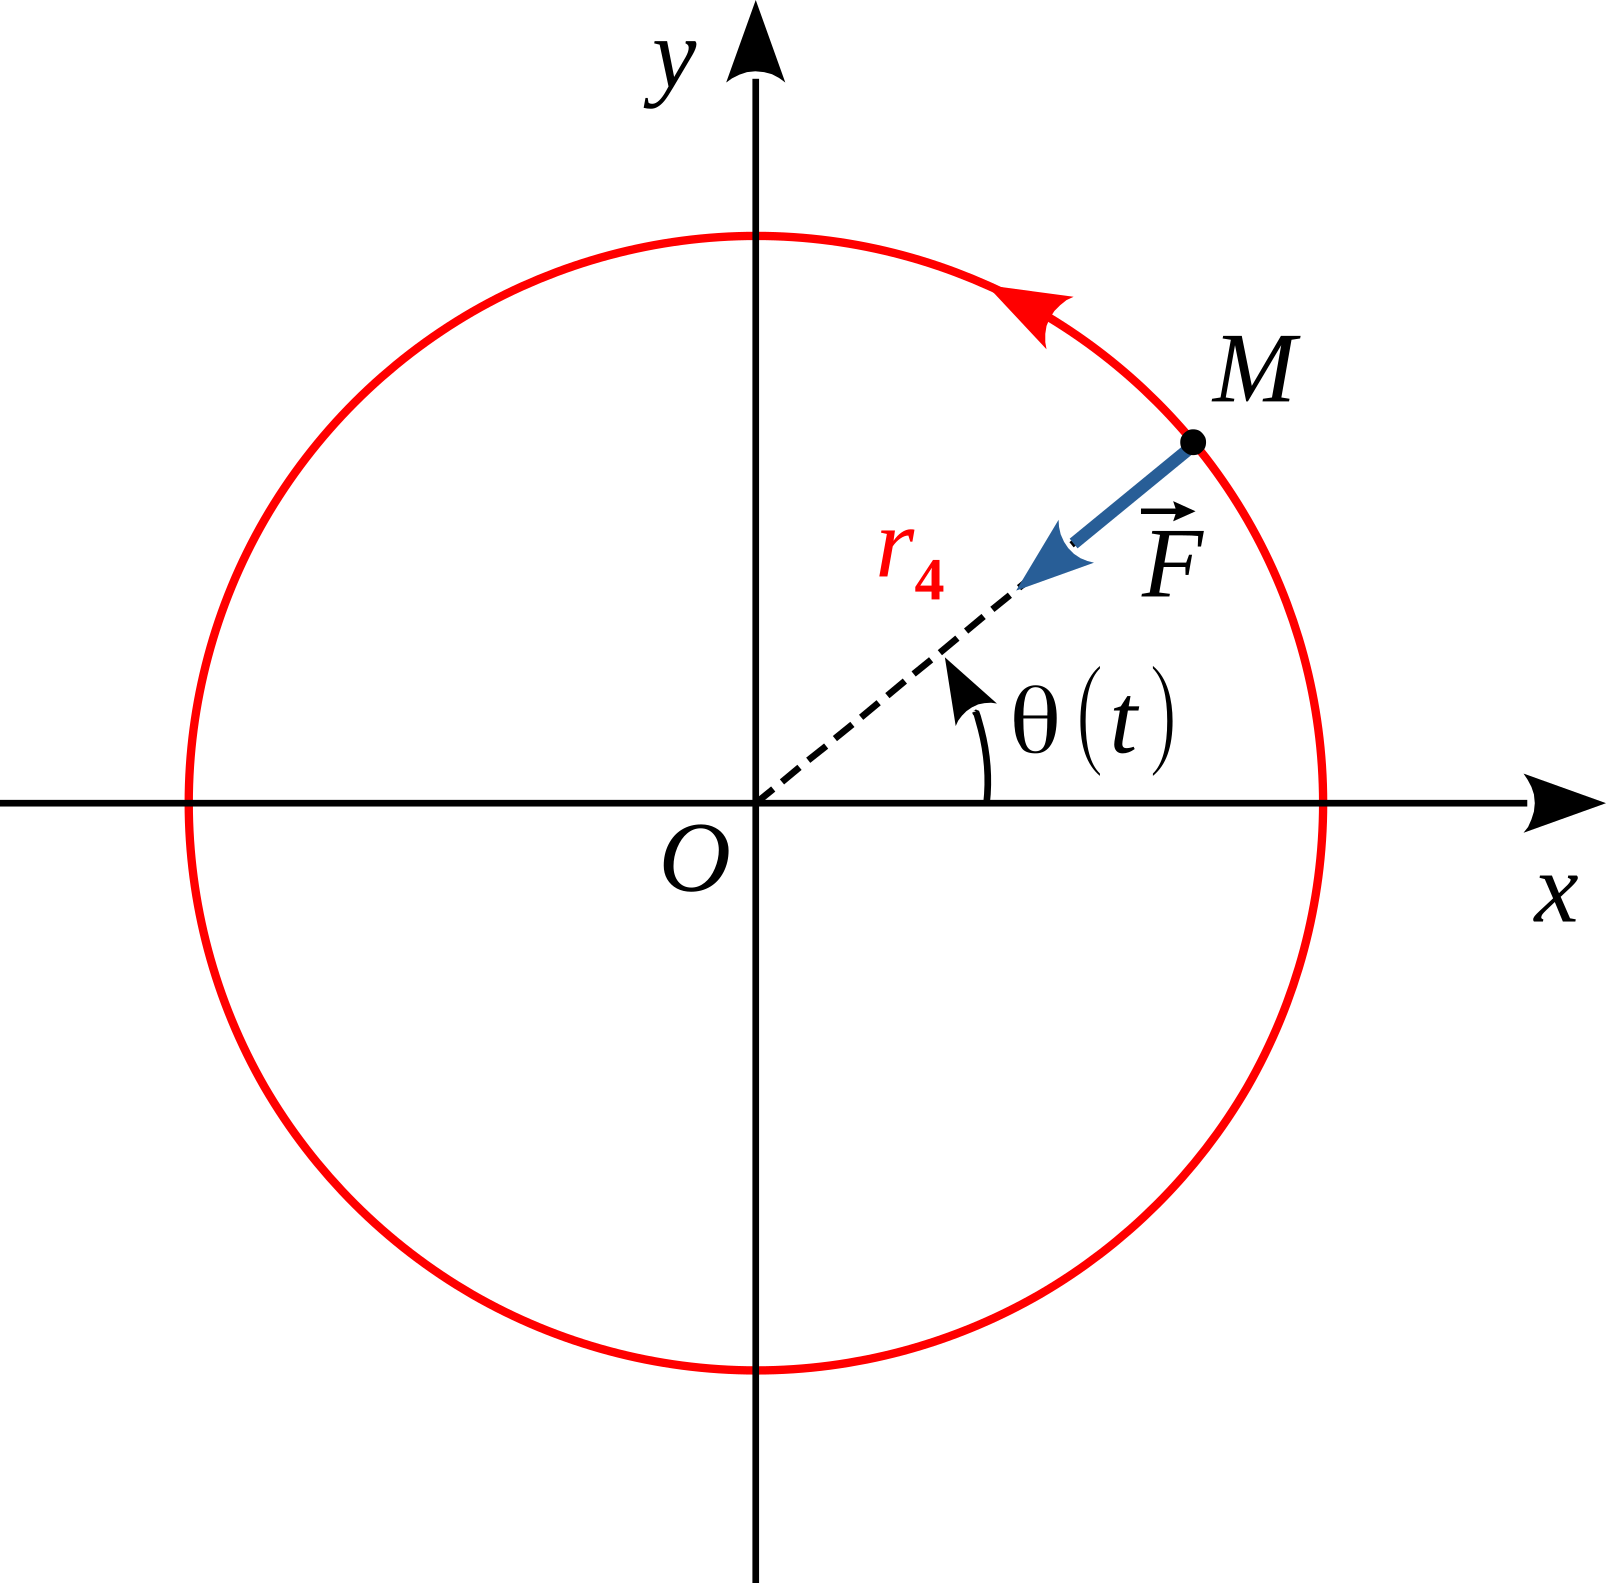
\includegraphics[scale=.7]{traj_att-color_cer}
%         \\
%         Trajectoire &
%         \textbf{parabolique} &
%         \textbf{circulaire}
%         \\\bottomrule
%     \end{tabularx}
% \end{table}

\begin{table}[h]
    \begin{tabularx}{\linewidth}{llYY}
        \toprule
        \multicolumn{2}{c}{Type de mouvement }
        & 
        \multicolumn{2}{c}{Caractéristiques}
        \\\midrule
        \textbf{Diffusion} & $0 \leq \Ec_m$ &
        $0 < \Ec_m < \infty$
        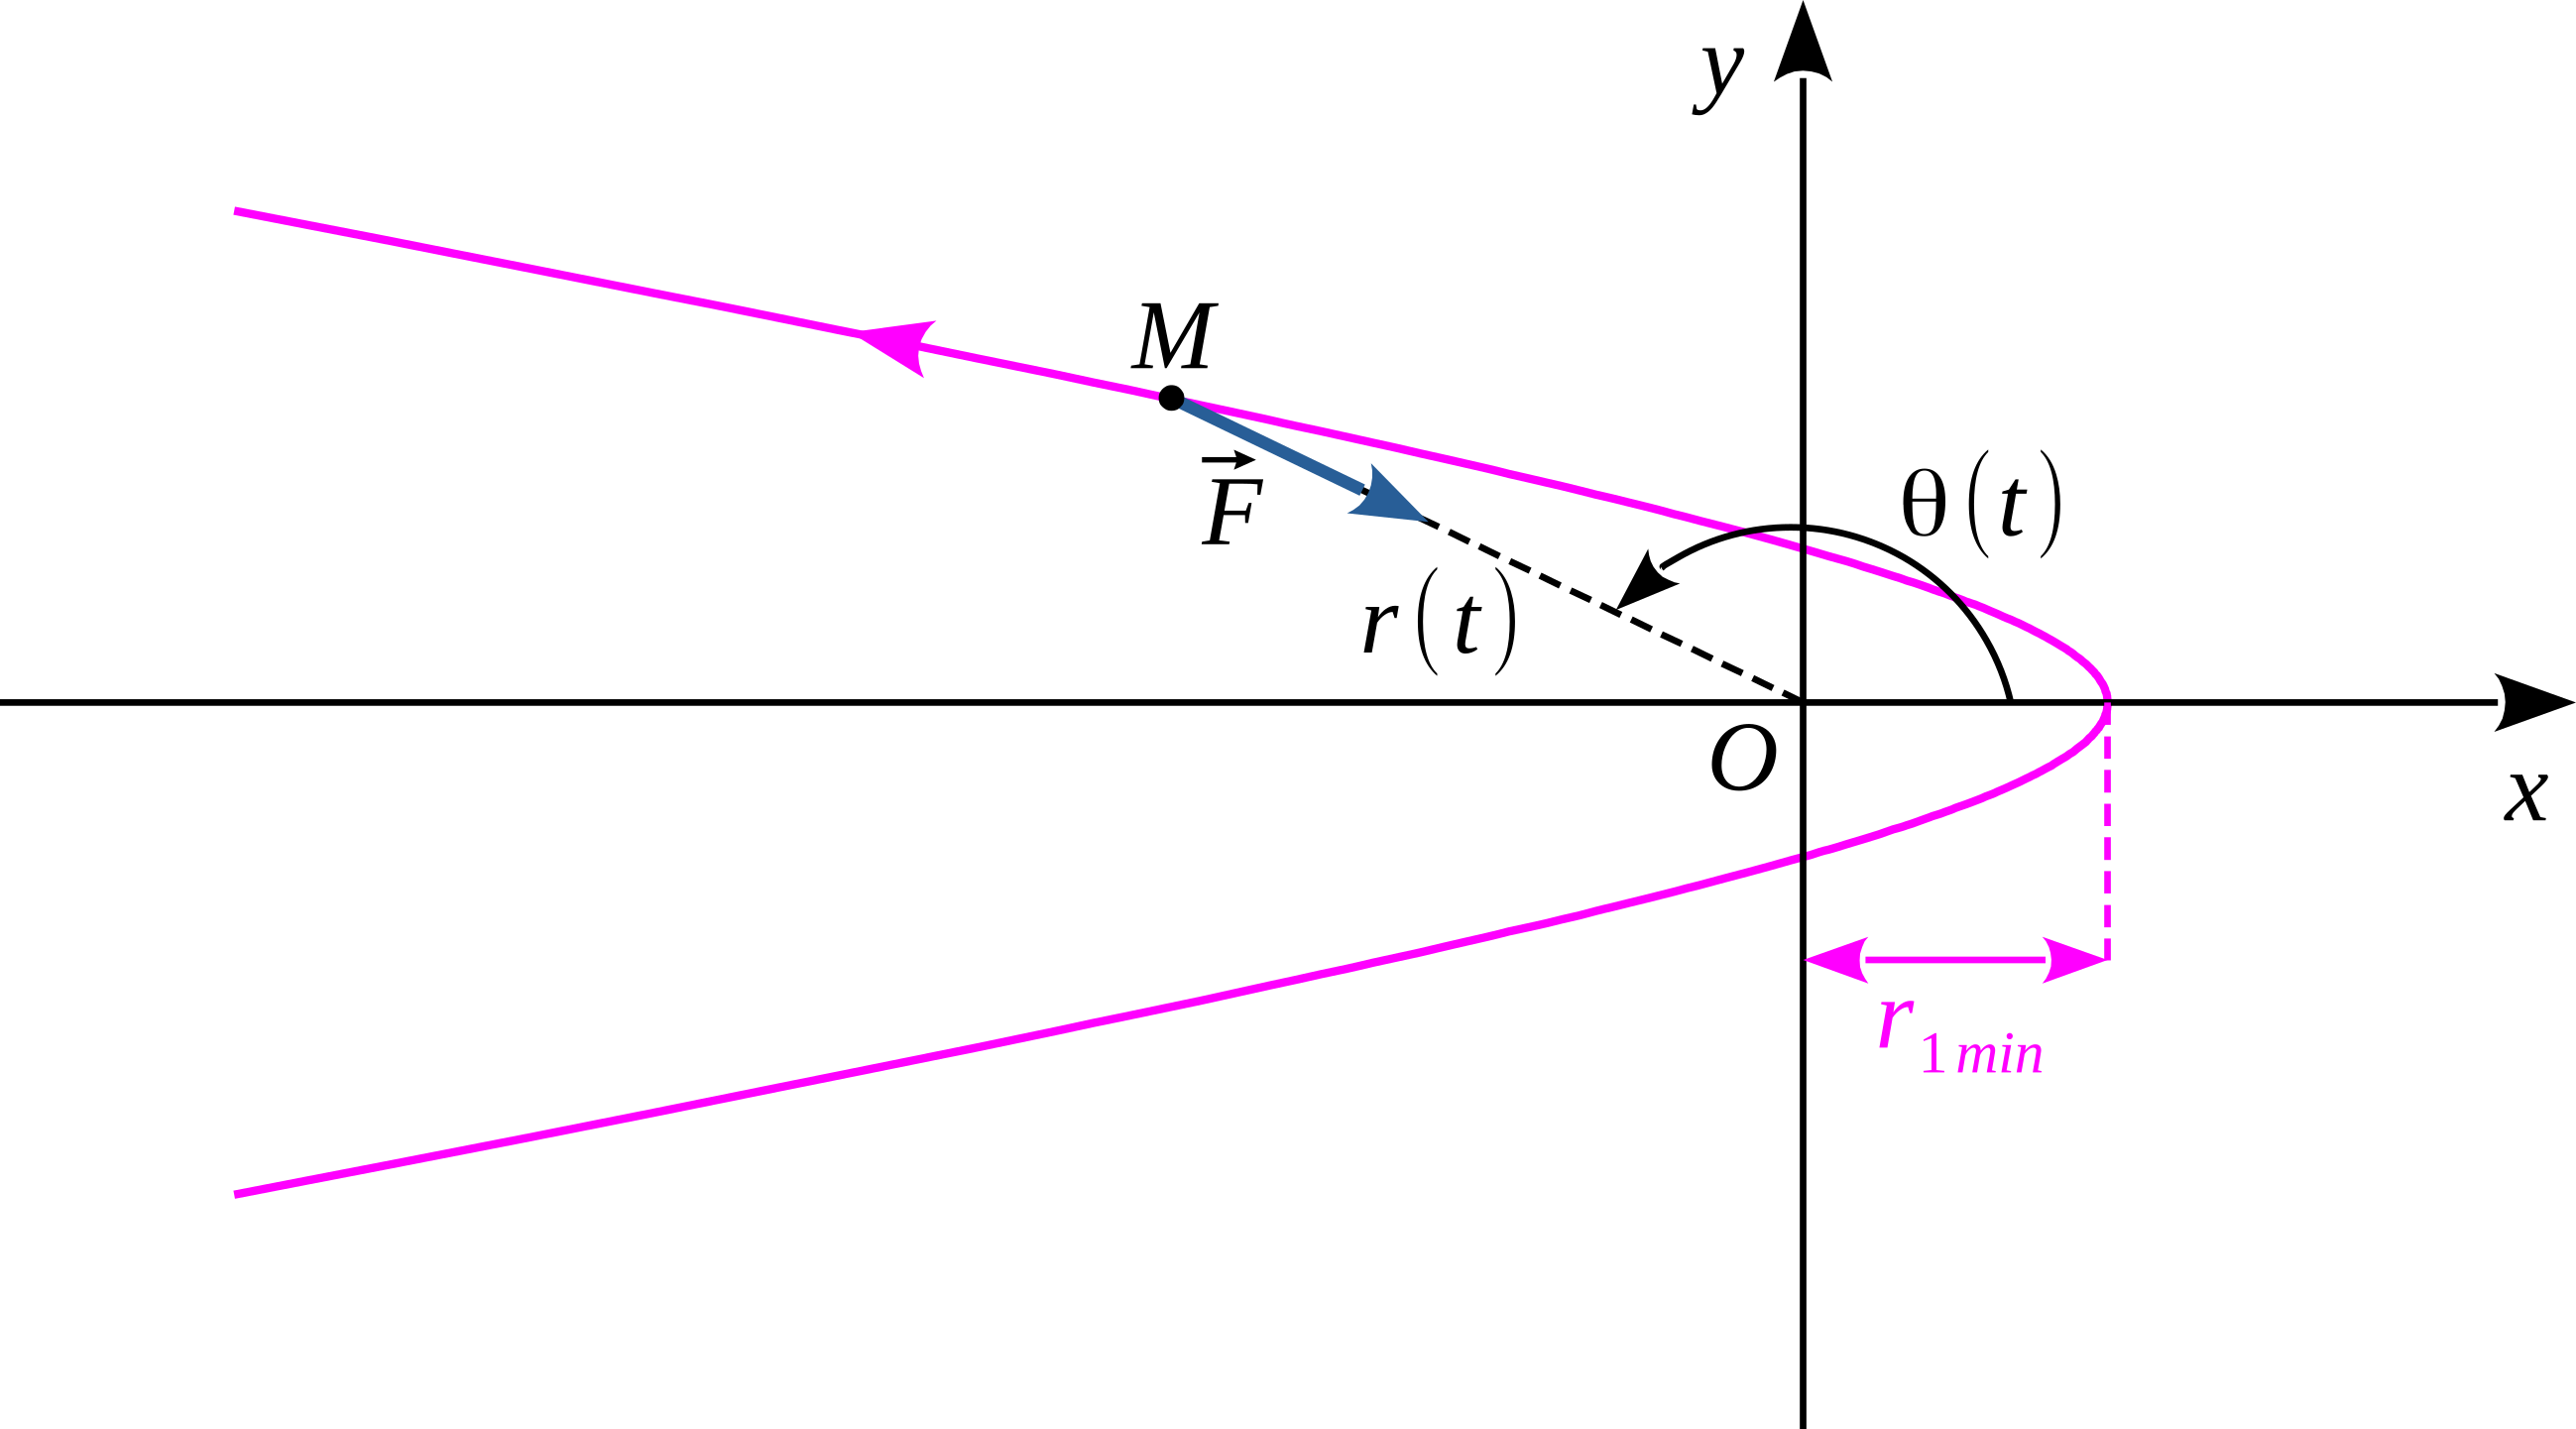
\includegraphics[width=\linewidth]{traj_att-color_hyp}
        Trajectoire \textbf{hyperbolique}
                                          &
        $\Ec_m = 0$
        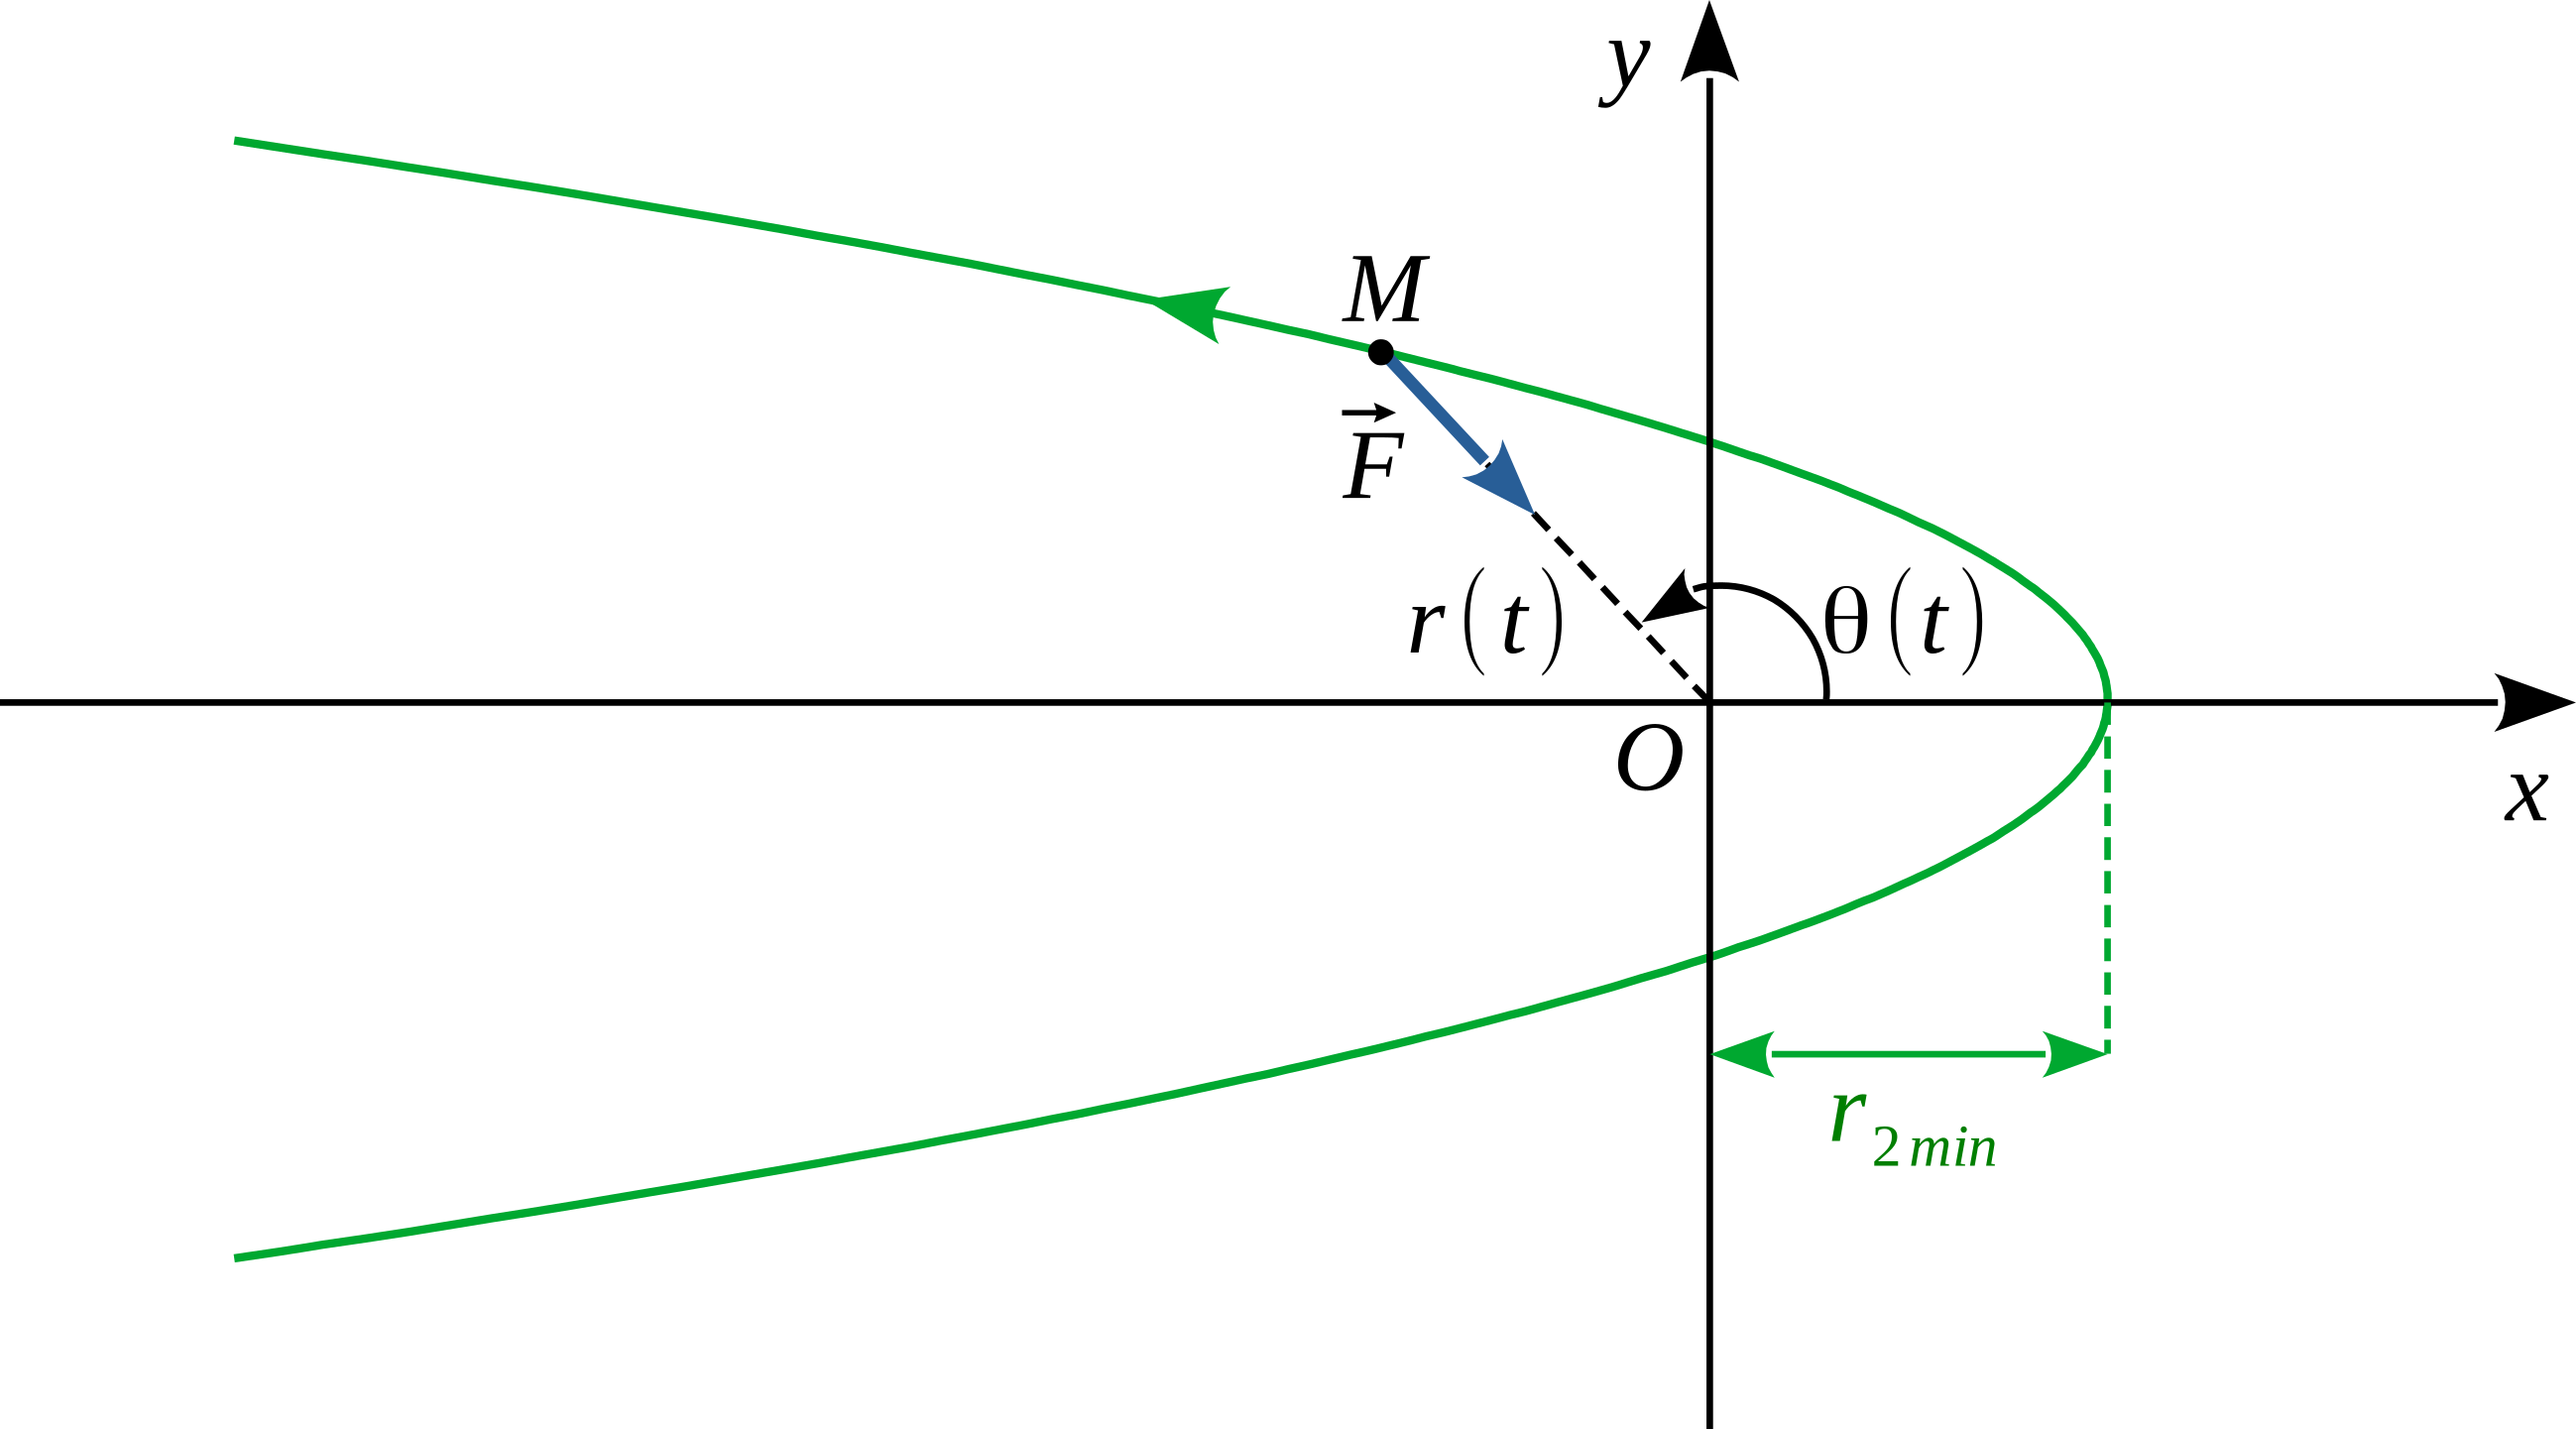
\includegraphics[width=\linewidth]{traj_att-color_par}
        Trajectoire \textbf{parabolique}
        \\\midrule
        \textbf{Lié} & $\Ec_m < 0$ &
        $-\Ec_0 < \Ec_m < 0$
        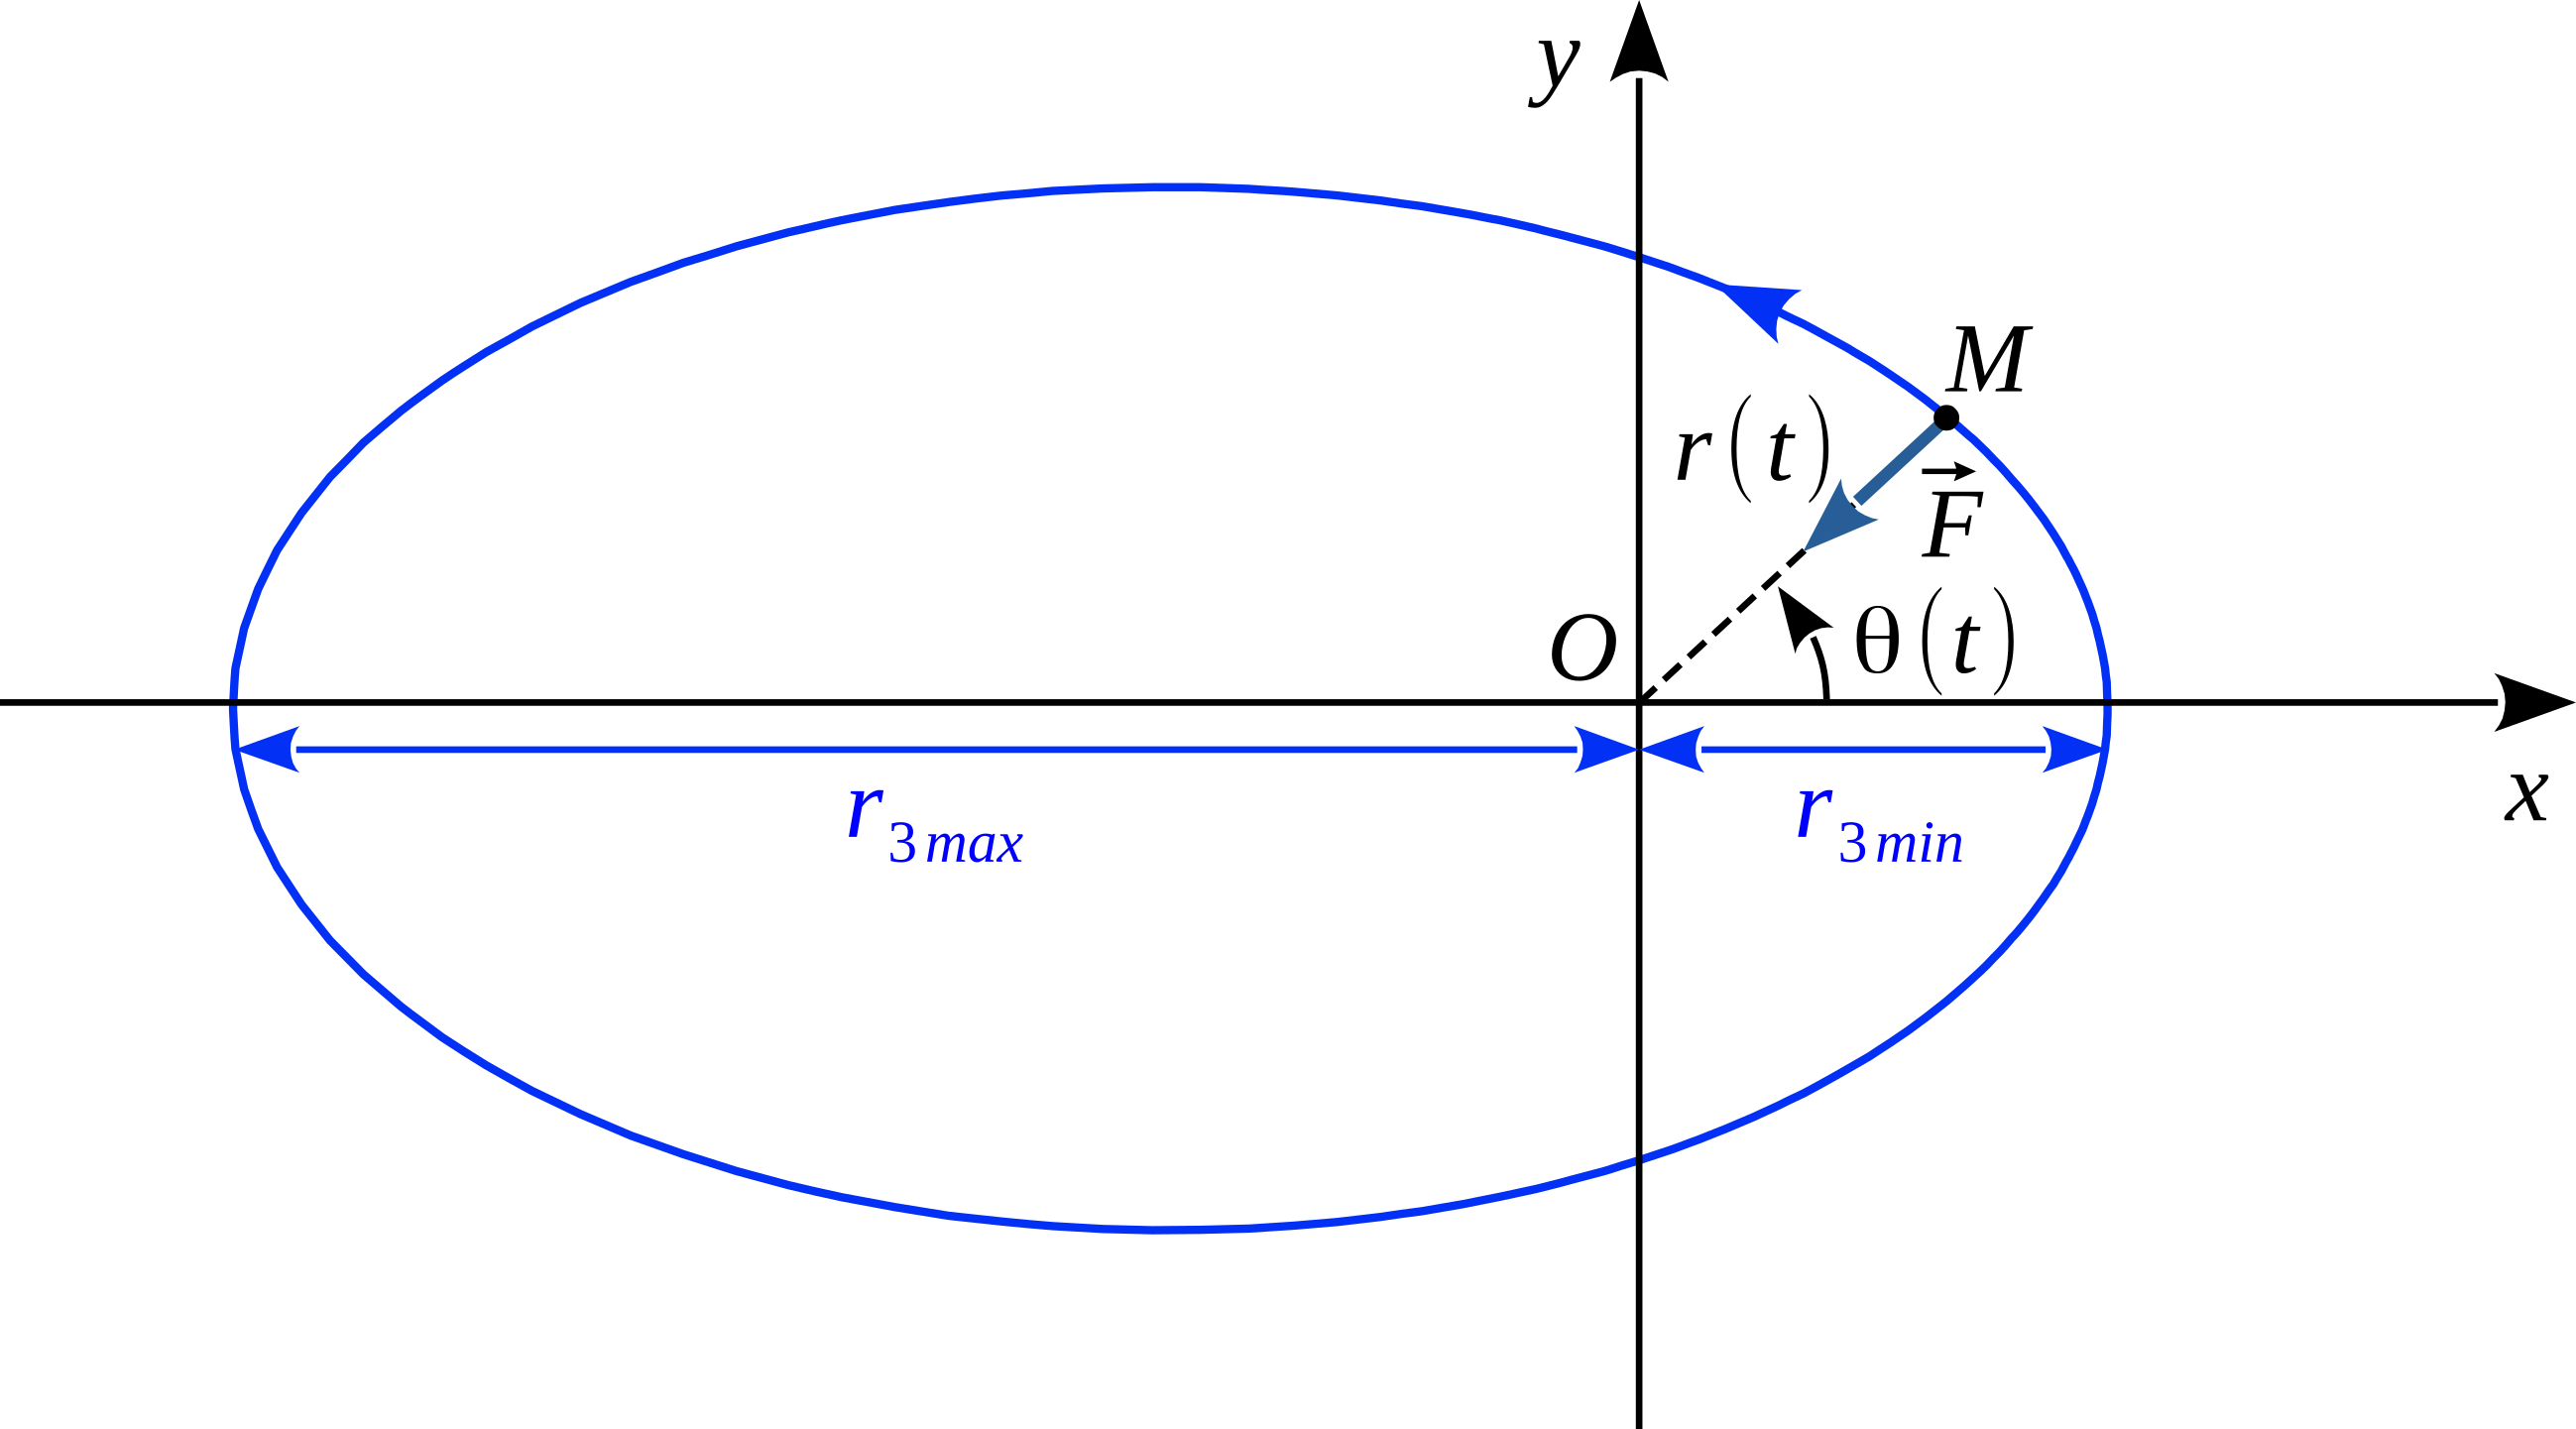
\includegraphics[width=\linewidth]{traj_att-color_ell}
        Trajectoire \textbf{elliptique}
                                 &
        $\Ec_m = -\Ec_0$
        \smallbreak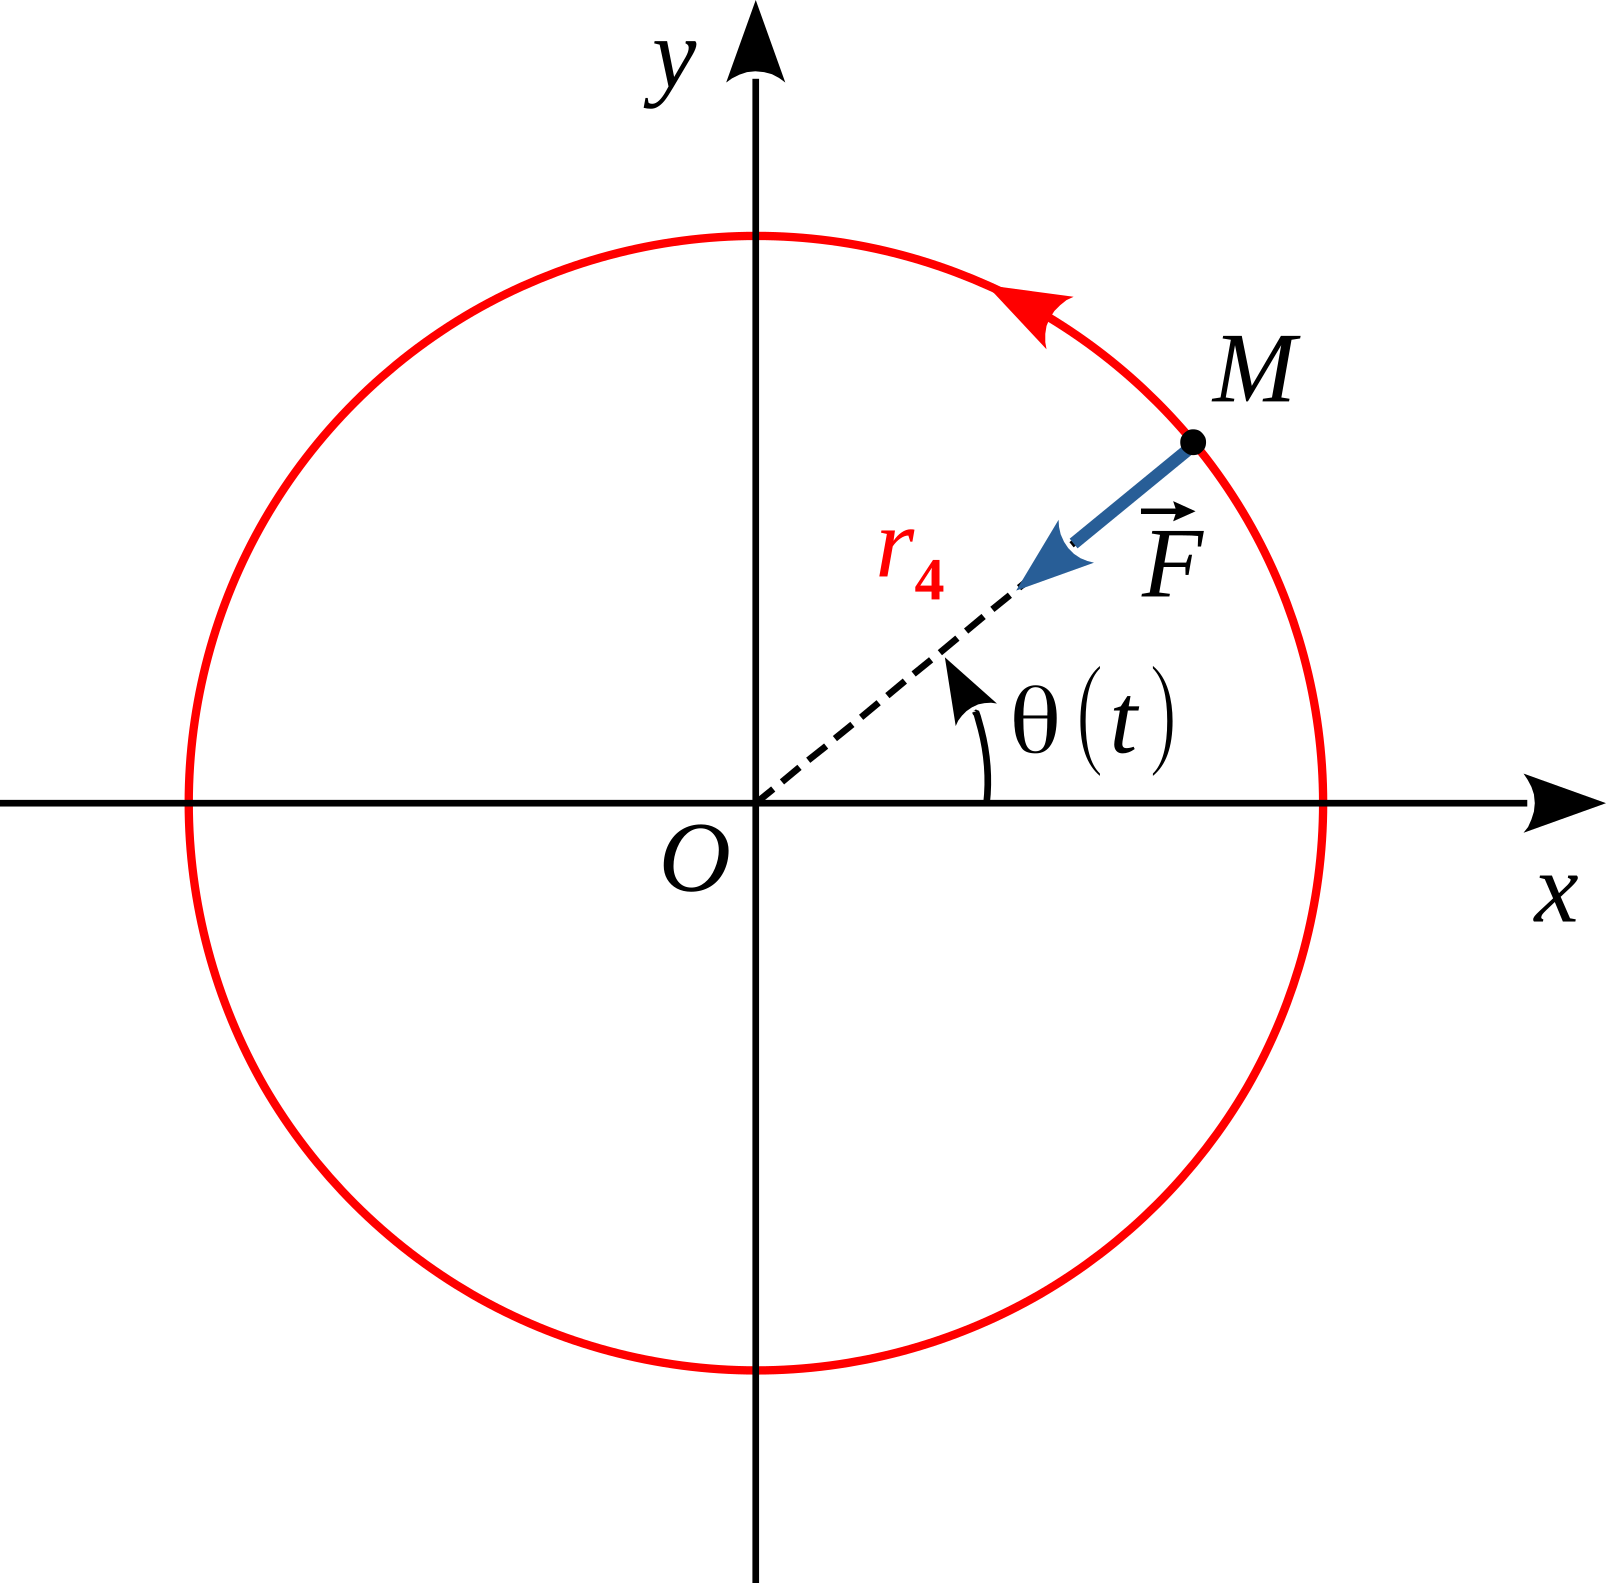
\includegraphics[scale=.6]{traj_att-color_cer}\smallbreak
        Trajectoire \textbf{circulaire}
        \\\bottomrule
    \end{tabularx}
\end{table}

\subsection{Cas répulsif}
Ce cas est bien plus simple~: la trajectoire est hyperbolique dans tous les cas.
\smallbreak
\begin{minipage}[c]{0.48\linewidth}
    \begin{center}
        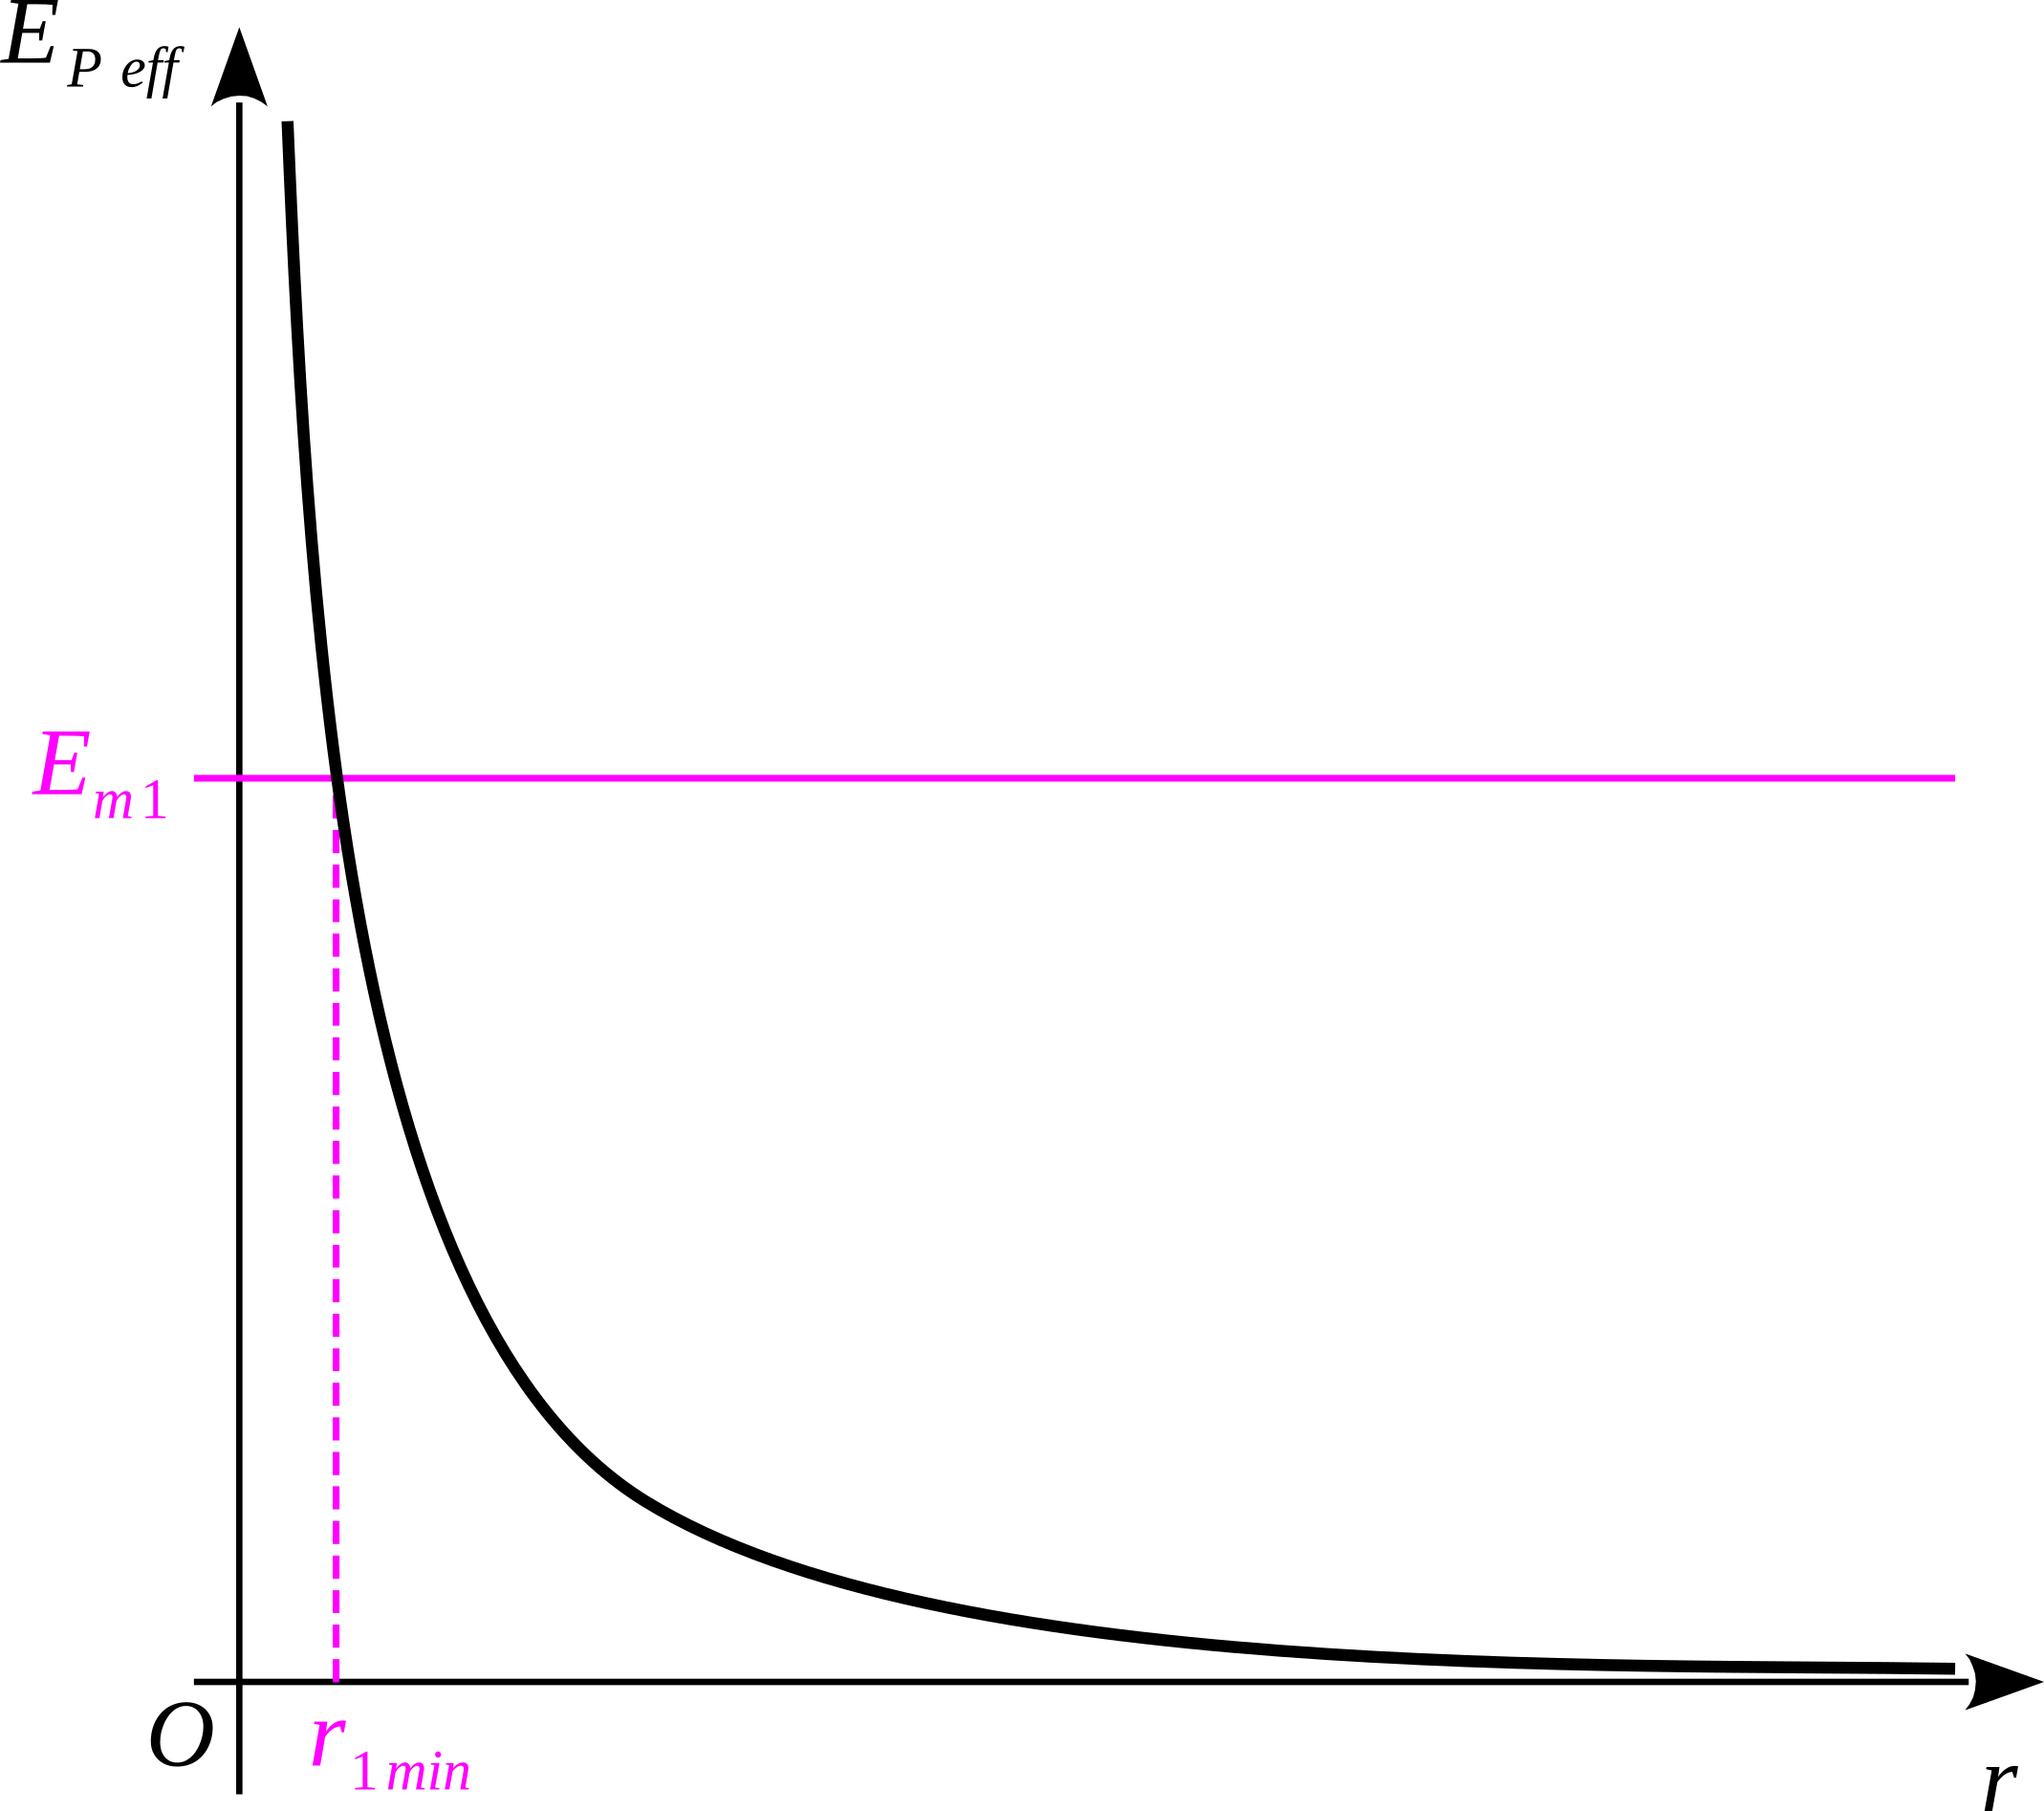
\includegraphics[height=5cm]{ep_eff-rep_color}
    \end{center}
\end{minipage}
\hfill
\begin{minipage}[c]{0.48\linewidth}
    \begin{center}
        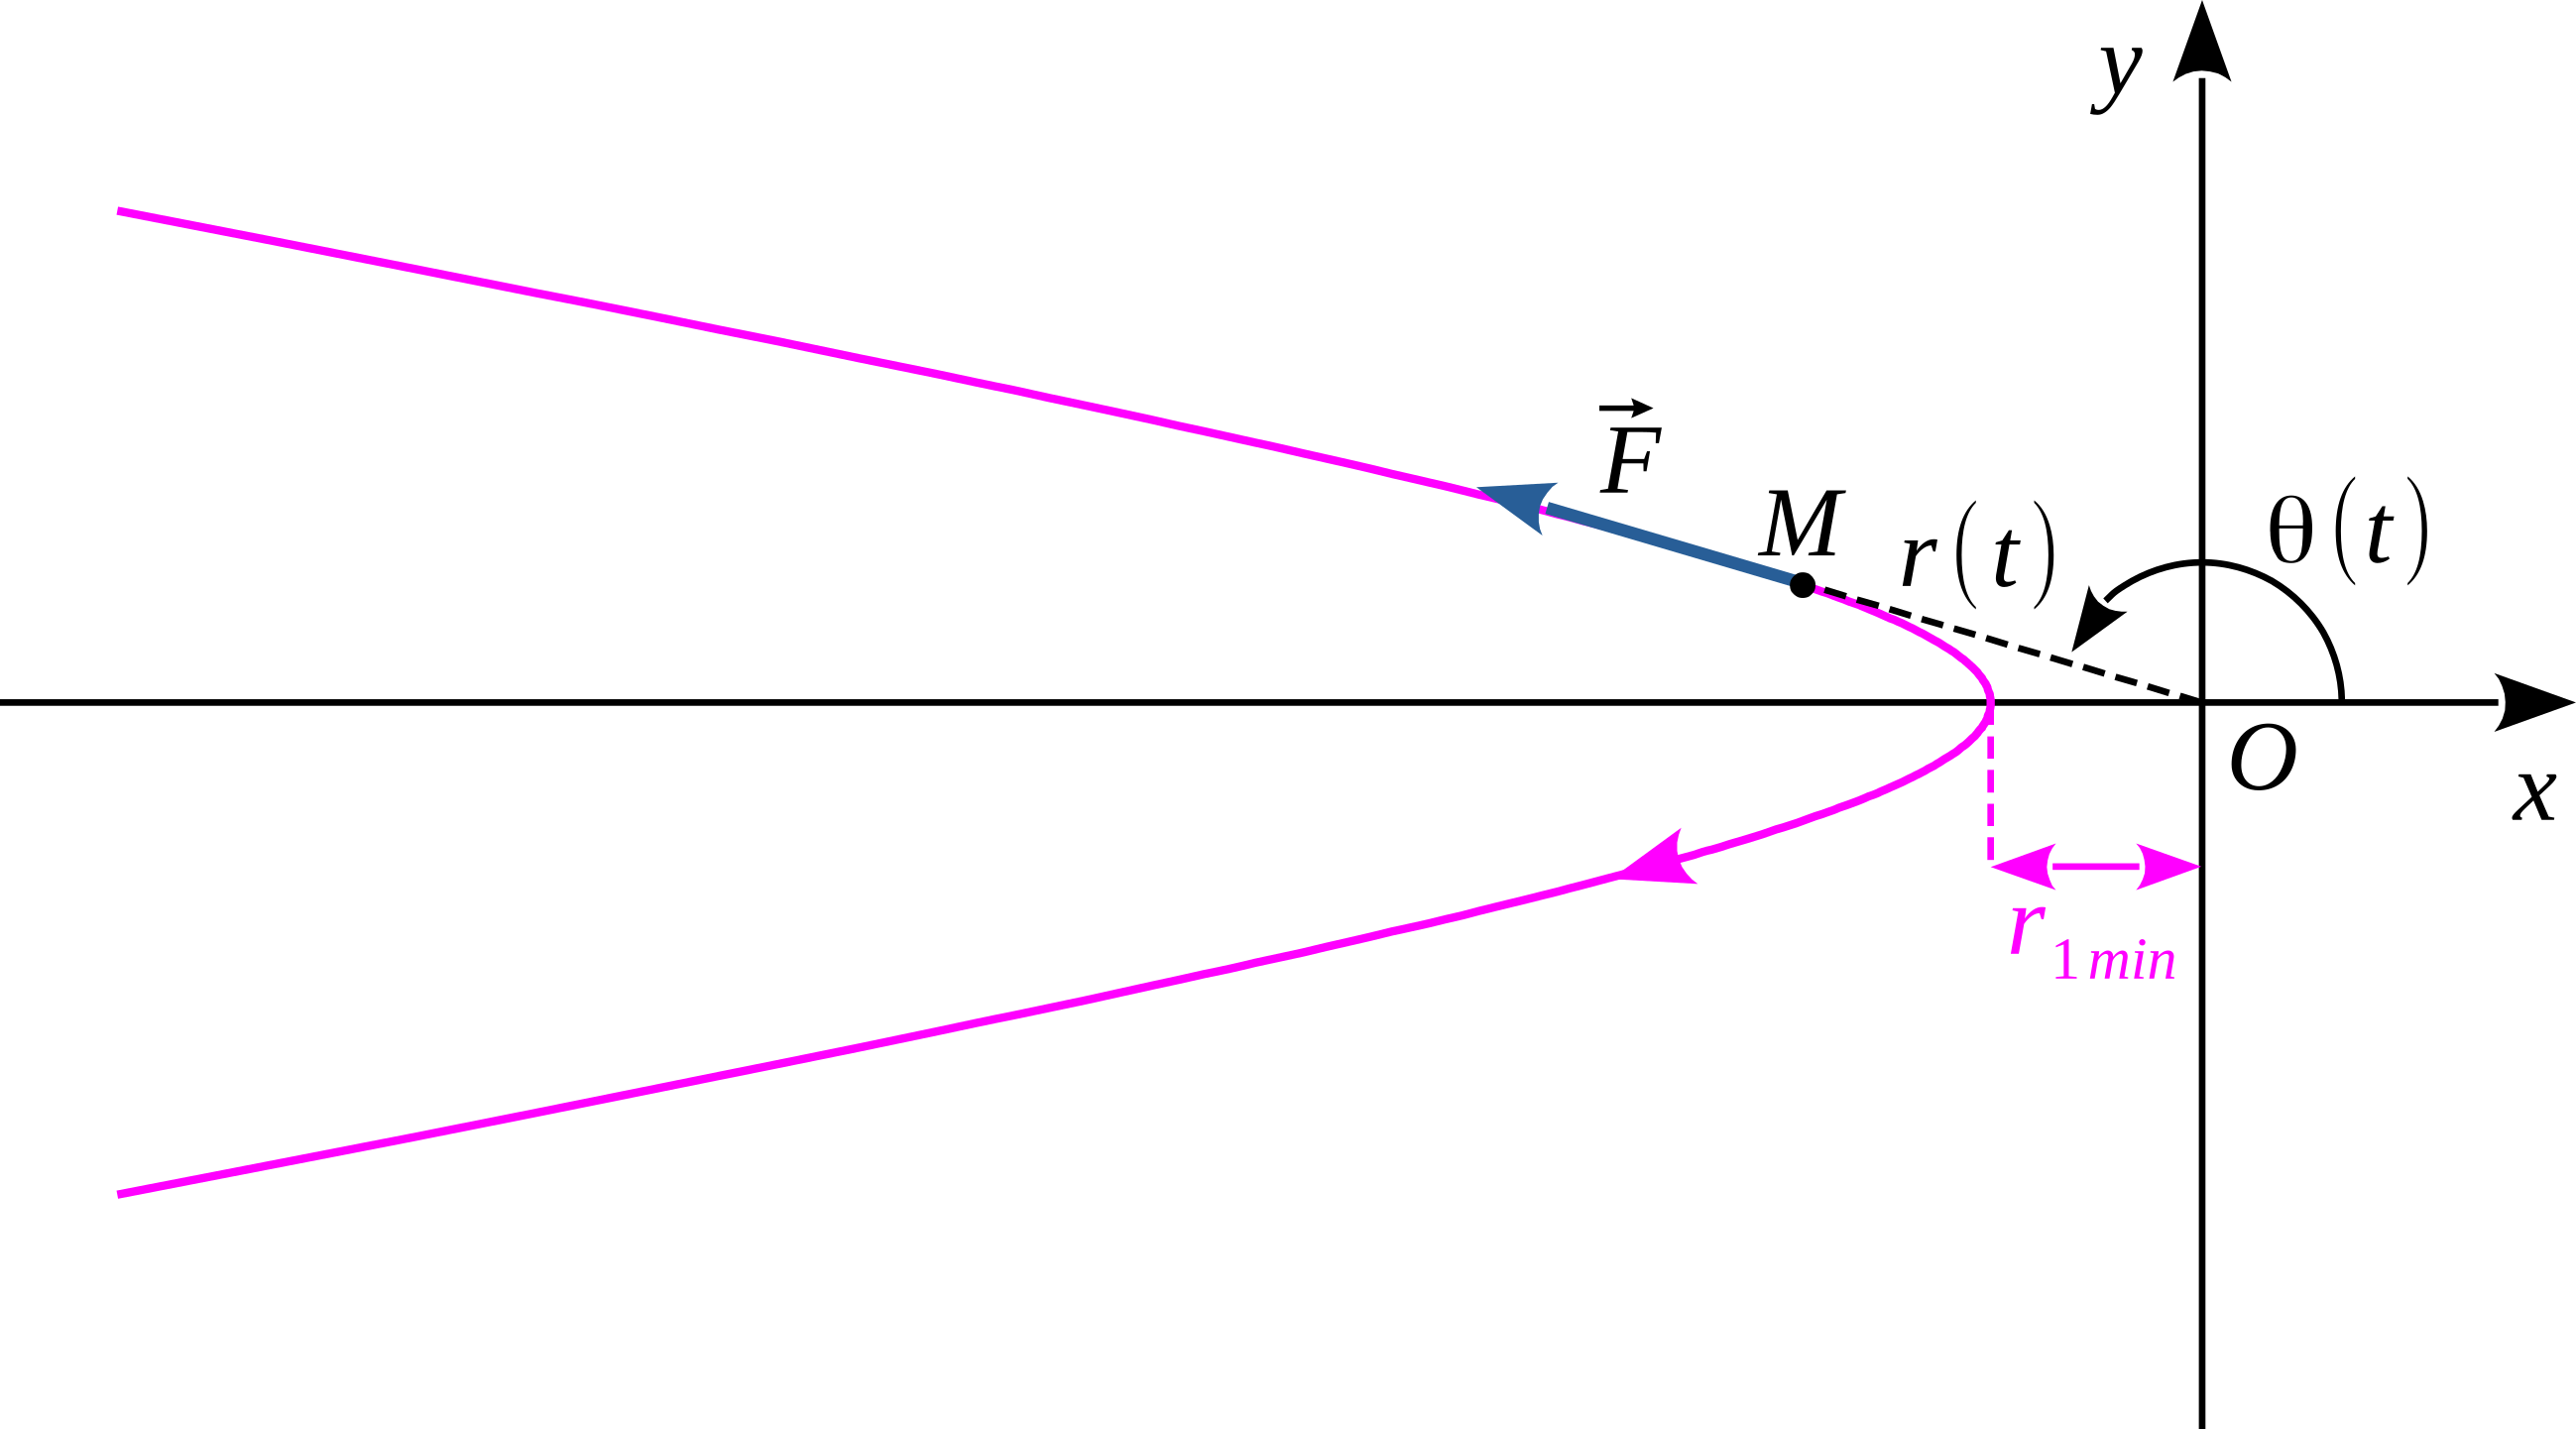
\includegraphics[height=5cm]{traj_rep-color}
    \end{center}
\end{minipage}

\section{Mécanique céleste}
\subsection{Qu'est-ce qu'une ellipse~?}
\begin{tdefi}{Définition~: ellipse}
    \begin{minipage}{0.45\linewidth}
        Analogue au cercle se définissant par l'ensemble des points M à égale
        distance du centre, une ellipse se définit comme l'ensemble des points M
        tels que
        \[{\rm MF}+{\rm MF'} = 2a\]
        avec F et F' les \textbf{foyers} de l'ellipse, et son $a$ demi-grand axe.
    \end{minipage}
    \hfill
    \begin{minipage}{0.45\linewidth}
        \begin{center}
            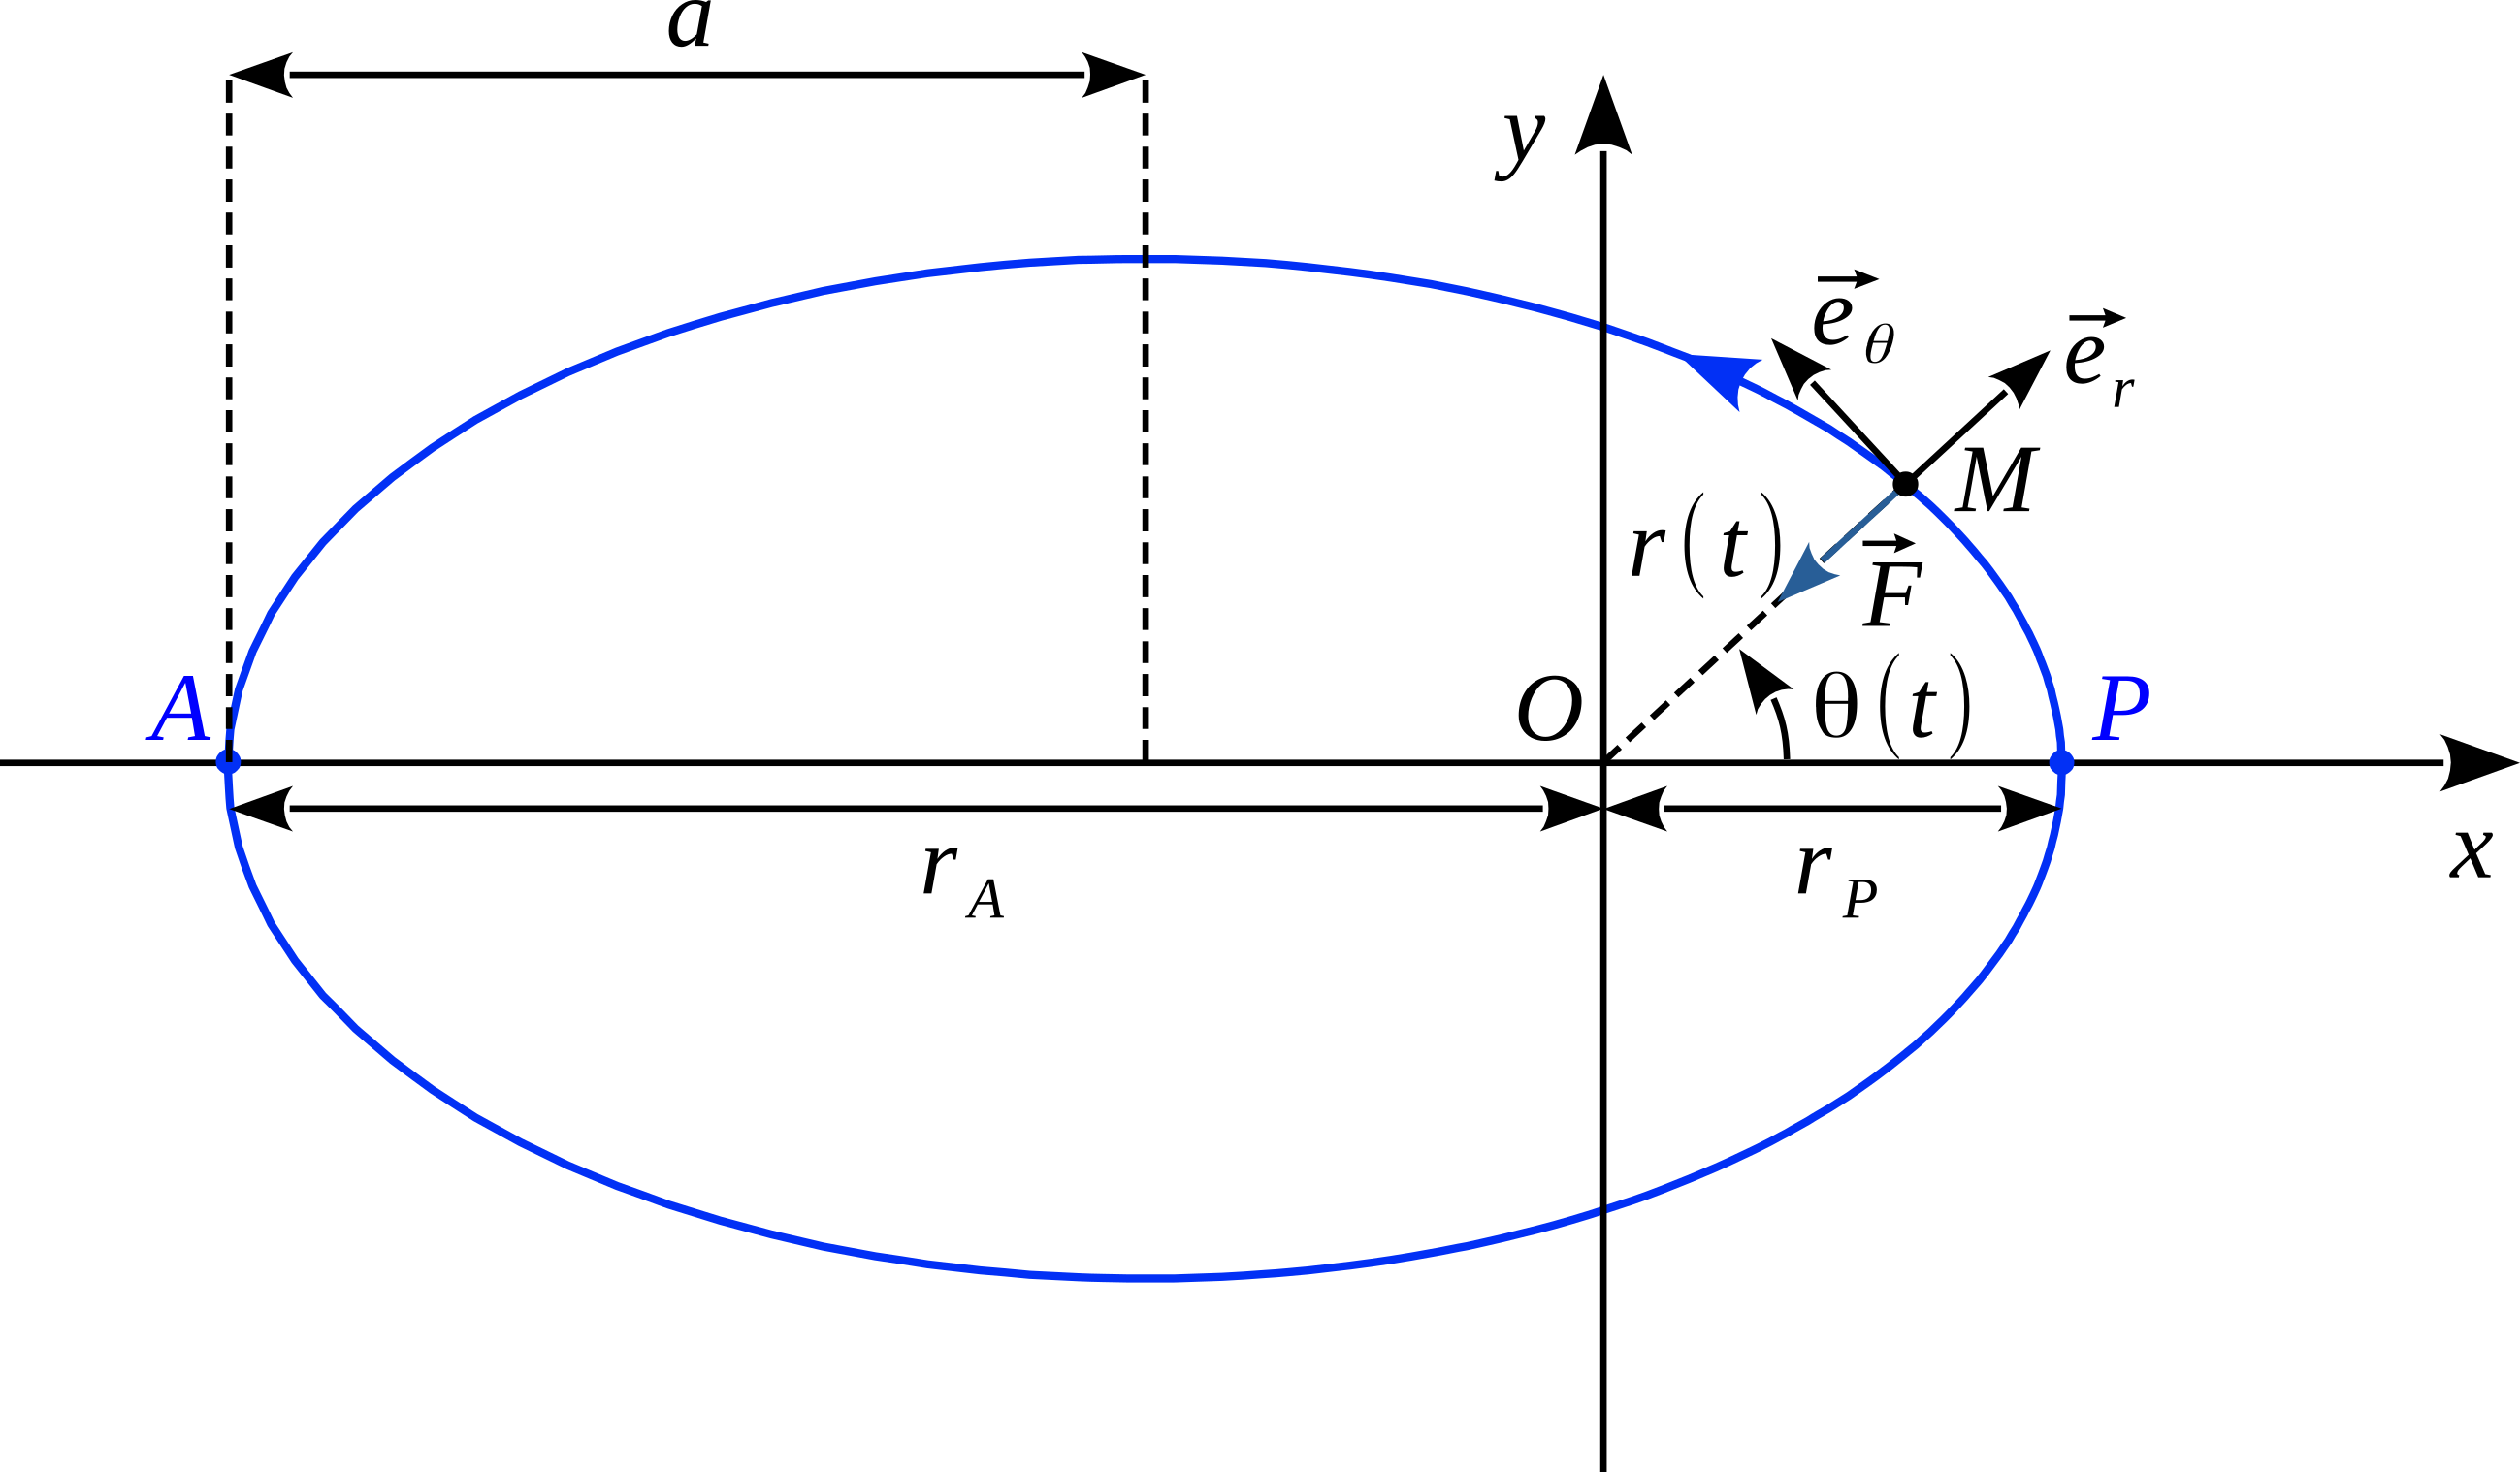
\includegraphics[width=\linewidth]{ell_def}
        \end{center}
    \end{minipage} \smallbreak
    Le point le plus proche de O, noté P, s'appelle le
    \textbf{péricentre}\footnote{Périgée pour la Terre, périhélie pour le
    Soleil}~; le point le plus éloigné de O, noté A, s'appelle
    l'\textbf{apocentre}\footnote{Apogée pour la Terre, aphélie pour le Soleil}.
    Les rayons $r_{\rm P}$ et $r_{\rm A}$ sont reliés à $a$ tels que
    \[\boxed{r_{\rm P} + r_{\rm A} = 2a}\]
\end{tdefi}

\subsection{Lois de \textsc{Kepler}}
Les lois de \textsc{Kepler} ont été établies par Johannes \textsc{Kepler} au
début du \textsc{XVII}\ieme\ siècle (publiées en 1609 et 1619) à partir de
relevés expérimentaux effectués par Tycho \textsc{Brahe} à la fin du
\textsc{XVI}\ieme\ siècle. \bigbreak
La première loi de \textsc{Kepler} précise la nature des trajectoires des
planètes.
\begin{tprop}{Première loi de \textsc{Kepler}, heart}
    \centering
    Dans le référentiel héliocentrique, les orbites des planètes sont des
    ellipses dont le centre du Soleil est l'un des foyers.
    \begin{center}
        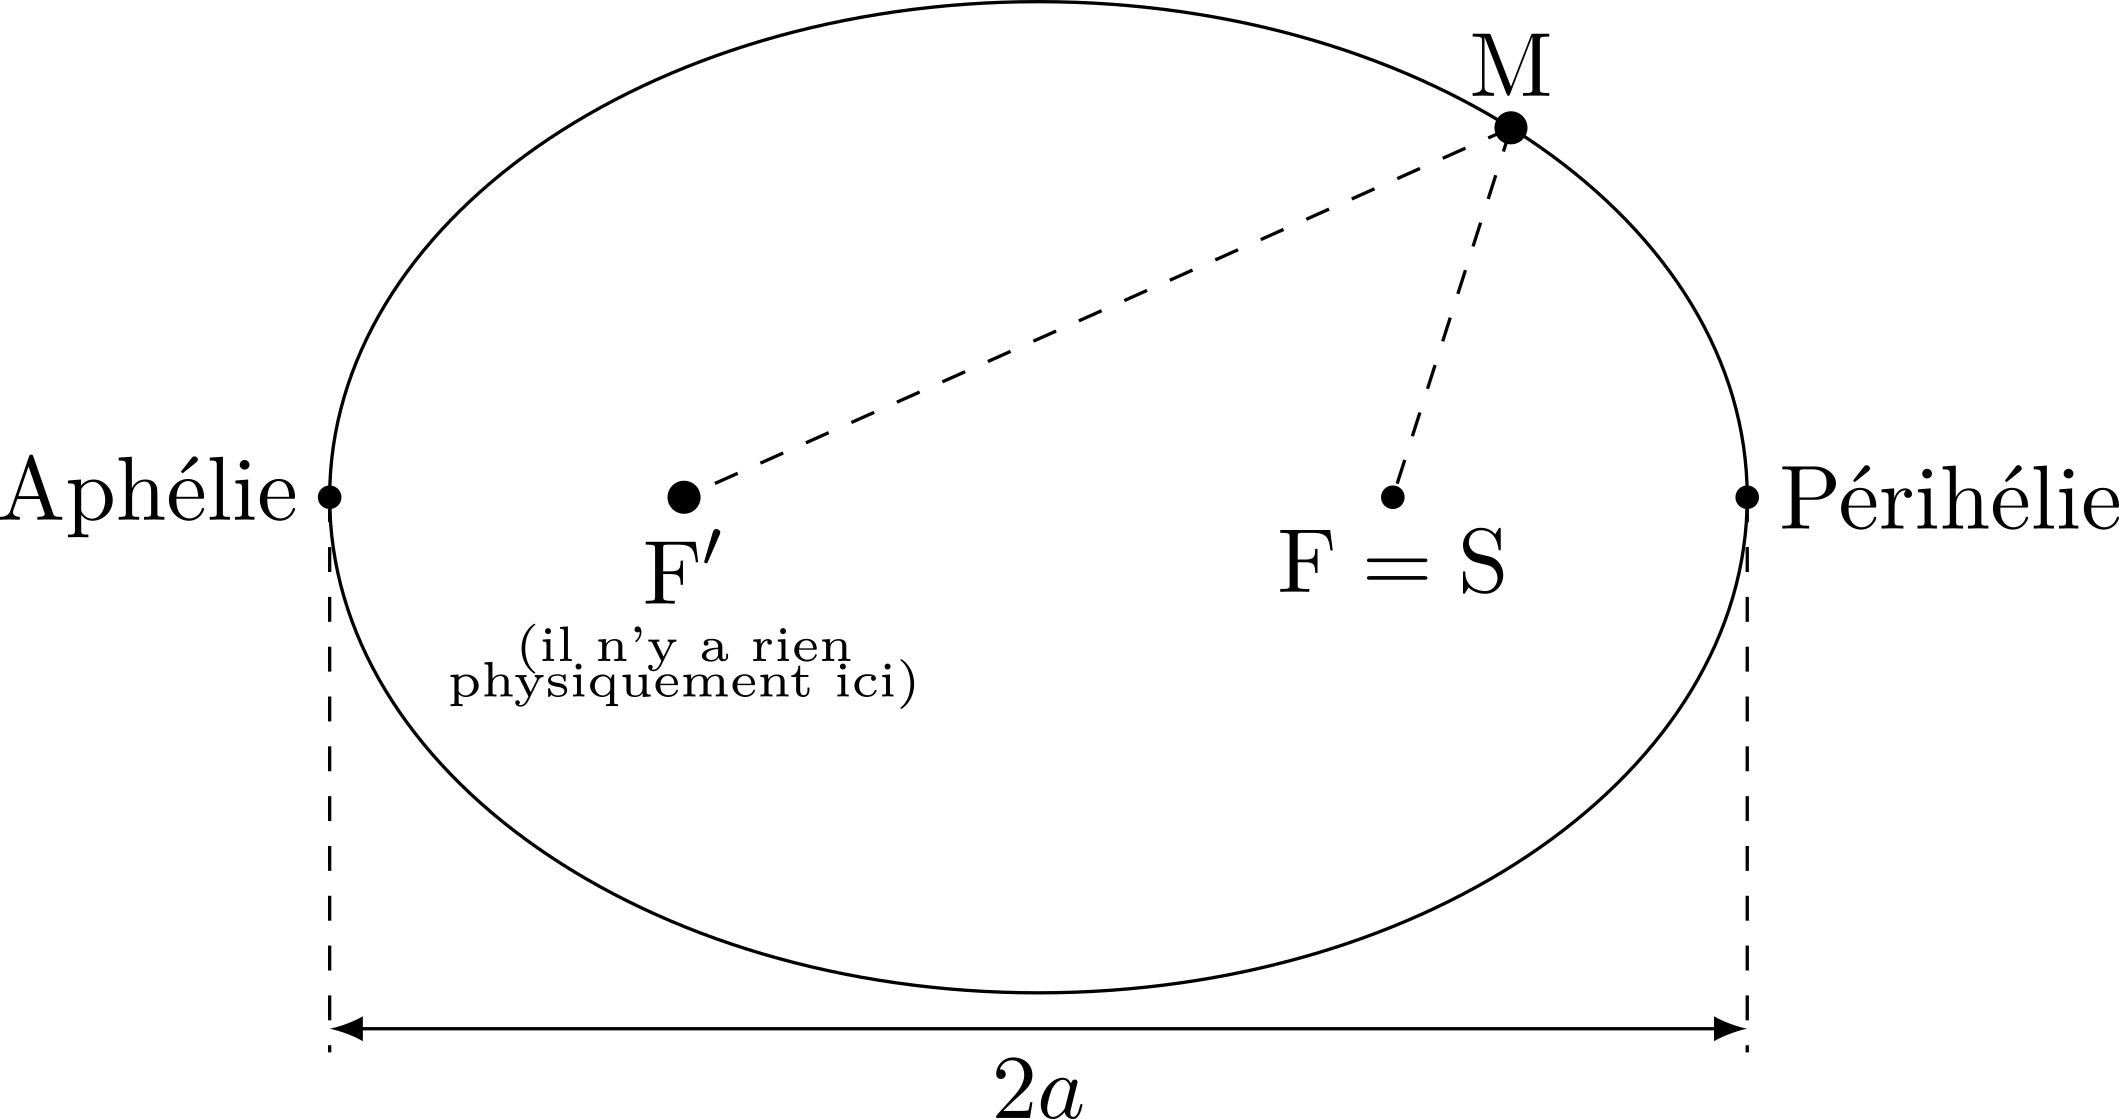
\includegraphics[scale=1]{kepler_1}
    \end{center}
\end{tprop}

Nous avons déjà déterminé la deuxième loi de \textsc{Kepler}, conséquence
directe de la conservation du moment cinétique.

\begin{tprop}{Deuxième loi de \textsc{Kepler}, heart}
    Pendant une durée donnée $\Dt$, l'aire $\D\Ac$ balayée par le rayon joignant
    le centre du Soleil au centre de la planète est constante.
\end{tprop}

La troisième et dernière loi de \textsc{Kepler} relie le demi-grand axe de
l'orbite à sa période~:
\begin{tprop}{Troisième loi de \textsc{Kepler}, heart}
    La période de révolution d'une planète autour du Soleil est reliée au
    demi-grand axe de son ellipse par~:
    \[\boxed{\frac{T^2}{a^3} = \frac{4\pi^2}{\Gc M_\Sr}}\]
\end{tprop}
\begin{rexem}{Exemple}
    Calculer la période de révolution de Mars autour du Soleil. On donne $a_{\rm
    Terre} = \SI{150e6}{km}$ et $a_{\rm Mars} = \SI{228e6}{km}$.
    \tcblower
    \begin{gather*}
        \frac{T_\Mr{}^2}{a_\Mr{}^3} =
        \frac{4\pi^2}{\Gc M_\Sr} =
        \frac{T_\Ter{}^2}{a_\Ter{}^3} 
        \\\Lra
        \boxed{T_\Mr = T_\Ter \sqrt{\frac{a_\Mr{}^3}{a_\Ter{}^3}}}
        \qavec
        \left\{
            \begin{array}{rcl}
                T_\Ter & = & \SI{1}{an}\\
                a_\Ter & = & \SI{150e6}{km}\\
                a_\Mr & = & \SI{228e6}{km}
            \end{array}
        \right.
        \\\AN
        \boxed{T_\Mr = \SI{1}{an}\,\SI{319}{jours}}
    \end{gather*}
\end{rexem}

\subsection{Mouvement circulaire}
\hspace*{-0.76cm}
\begin{minipage}[t]{0.70\linewidth}
    \begin{enumerate}[label=\sqenumi]
        \item{Système}~: \{planète\} assimilée à un point matériel M de masse $m$
        \item{Référentiel}~: héliocentrique, supposé galiléen.
        \item{Repère}~: cylindrique $(\Or,\ur,\ut)$ avec O centre du Soleil, R le
            rayon supposé constant ($\dot{R} = 0$).
        \item{Repérage}~:
            \begin{gather*}
                \OM = R\ur\\
                \vf = R\tp\ut\\
                \af = -R\tp^2\ur + R\tpp\ut
            \end{gather*}
    \end{enumerate}
\end{minipage}
\hfill
\begin{minipage}[t]{0.25\linewidth}
    ~\vspace*{-20pt}
    \begin{center}
        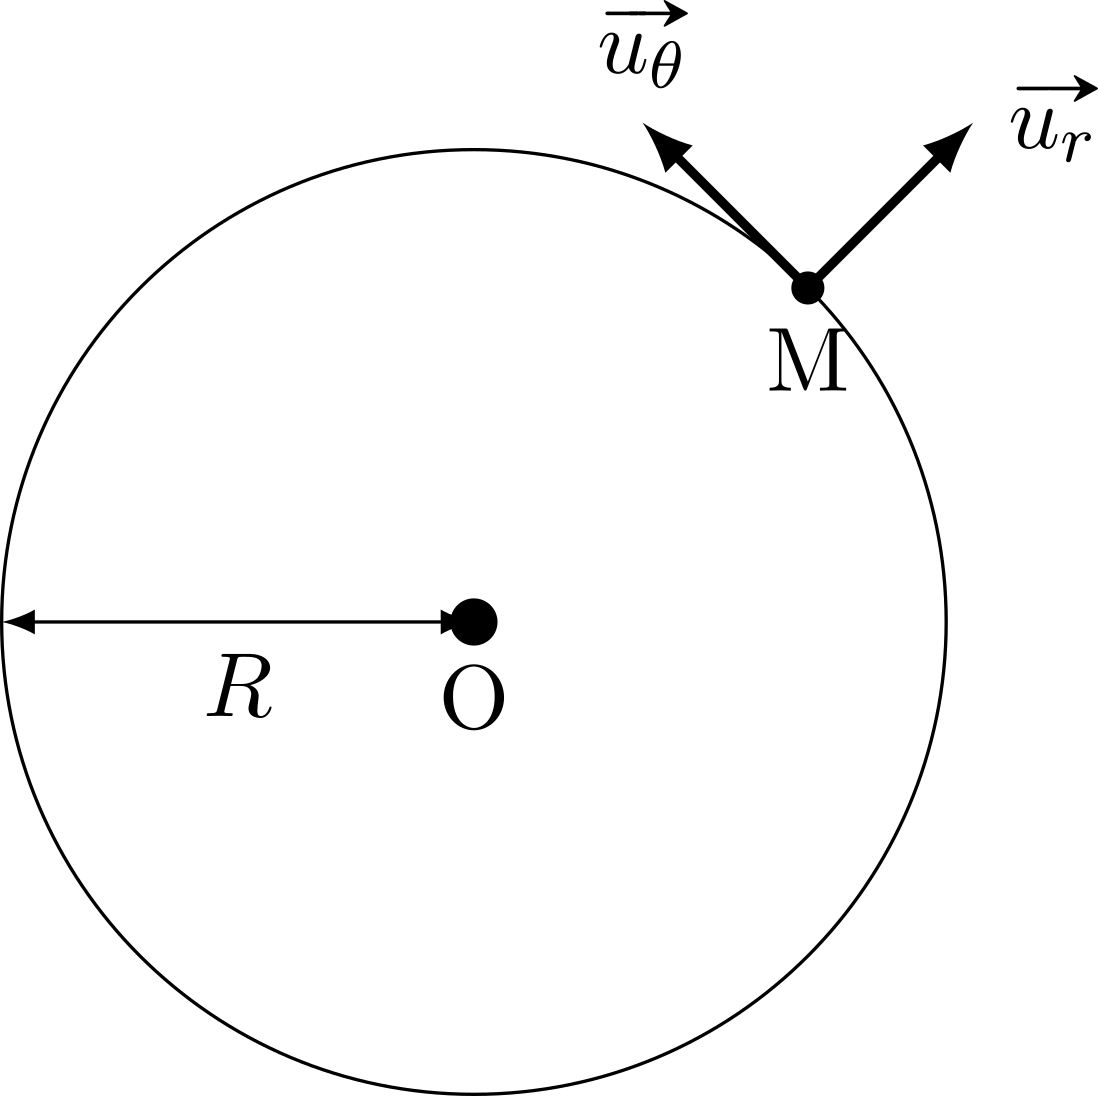
\includegraphics[width=\linewidth]{kepler_3_circ}
    \end{center}
\end{minipage}
\begin{enumerate}[label=\sqenumi, start=5]
    \item{Bilan des forces}~: force gravitationnelle $\DS\Ff = -\Gc
        \frac{mM_S}{R^2}\ur$ avec $M_S$ la masse du soleil.
    \item{PFD}~:
        \[m\af = \Ff\]
    \item{Équations scalaires}~:
        \begin{empheq}[left=\empheqlbrace]{align*}
            -mR\tp^2 &= -\Gc \frac{mM_S}{R^2}\ur\\
            mR\tpp &= 0
        \end{empheq}
    \item{Réponse aux questions}~: la deuxième équation donne $\tpp = 0 \Ra \tp
        = \cte$, et la première donne
        \[
            \boxed{\tp = \sqrt{\frac{\Gc M_S}{R^3}}}
            \Lra
            \boxed{v = \sqrt{\frac{\Gc M_S}{R}}}
        \]
\end{enumerate}
\begin{tror}{Important, hand, sidebyside}
    \begin{center}
        \begin{bfseries}
            Le mouvement \ul{circulaire} d'un astre autour d'un autre
            est nécessairement uniforme, et on a
            \[\boxed{v_{\rm cercle} = \sqrt{\frac{\Gc M_S}{R}}}\]
        \end{bfseries}
    \end{center}
    \tcblower
    \danger Le mouvement elliptique \textbf{n'est pas uniforme}~! On trouve
    de plus $\rp_{\rm P,A} = 0$ en tant que points extrema de $r(\tt)$, soit
    \textbf{en ces points} uniquement, $\vf_{\rm P,A} = r\tp\ut$. \danger
\end{tror}
\begin{enumerate}[label=\sqenumi]
    \item[] De plus, avec $T$ la période de révolution de l'astre, on a
        \begin{align*}
            \tp &= \frac{2\pi}{T}
            \\\Ra
            \frac{4\pi^2}{T^2} &= \frac{\Gc M_S}{R^3}
            \\\Lra
            \Aboxed{\frac{T^2}{R^3} &= \frac{4\pi^2}{\Gc M_S}}
        \end{align*}
\end{enumerate}
\begin{tror}{Important, hand, sidebyside}
    \begin{center}
        \begin{bfseries}
            La période de révolution du mouvement \ul{circulaire} d'un astre
            autour d'un autre vérifie
            \[\boxed{\frac{T^2}{R^3} = \frac{4\pi^2}{\Gc M_S}}\]
        \end{bfseries}
    \end{center}
    \tcblower
    On admet que \textbf{le résultat s'étend à une trajectoire elliptique en
    remplaçant le rayon $R$ par le demi-grand axe $a$}.
\end{tror}
\begin{enumerate}[label=\sqenumi]
    \item[] Enfin, avec l'énergie mécanique, on a
        \begin{align*}
            \Ec_m &= \underbracket[1pt]{\cancel{\frac{1}{2}m\dot{R}^2}}_{=0} +
            \frac{1}{2}mR^2\tp^2 - \Gc\frac{mM_S}{R}
            \\\Lra
            \Ec_m &= \frac{1}{2}m\frac{\Gc M_S}{R} - \Gc\frac{mM_S}{R}
            \\\Lra
            \Aboxed{\Ec_m &= -\Gc\frac{mM_S}{2R}}
        \end{align*}
\end{enumerate}
\begin{tror}{Important, hand, sidebyside}
    \begin{center}
        \begin{bfseries}
            L'énergie mécanique du mouvement \ul{circulaire} d'un astre autour
            d'un autre vérifie
            \[\boxed{\Ec_{m,\rm cercle} = -\Gc\frac{mM_S}{2R}}\]
        \end{bfseries}
    \end{center}
    \tcblower
    On admet que \textbf{le résultat s'étend à une trajectoire elliptique en
    remplaçant le rayon $R$ par le demi-grand axe $a$}.
\end{tror}

\section{Satellite en orbite terrestre}
On se place ici dans le référentiel géocentrique, afin de traiter le mouvement
d'un satellite autour de la Terre.
\subsection{Vitesses cosmiques}
\subsubsection{Première vitesse cosmique}
\begin{tdefi}{Définition~: première vitesse cosmique}
    La première vitesse cosmique, ou vitesse de \textbf{satellisation minimale},
    est la vitesse minimale à fournir à un objet situé sur Terre pour pouvoir le
    placer en orbite \textbf{circulaire} autour de la Terre.
\end{tdefi}
\begin{tprop}{Première vitesse cosmique}
    Sur Terre, on trouve
    \[
        \boxed{v_c \approx \sqrt{\frac{\Gc m_\Ter}{R_\Ter}} \approx
        \SI{8}{km.s^{-1}}}
    \]
\end{tprop}
\begin{tdemo}{Démonstration~: première vitesse cosmique}
    Pour satelliser un corps, il faut faire varier son énergie mécanique d'un
    état où il est au sol à un état où il est en orbite. La plus petite énergie
    mécanique pour cela est celle que l'on vient de déterminer dans l'étude de
    la trajectoire circulaire. Ainsi, à partir de l'énergie mécanique d'un objet
    lancé au niveau du sol, on a
    \begin{gather*}
        \Ec_{m,\rm sol} = \frac{1}{2}mv^2 -\Gc \frac{mM_\Ter}{R_\Ter}
        \qet
        \Ec_{m,\rm cercle} = -\Gc \frac{mM_\Ter}{2R_\Ter}
        \\\Lra
        \frac{1}{2}mv_c{}^2 -\Gc \frac{mM_\Ter}{R_\Ter} = -\Gc \frac{mM_\Ter}{2R_\Ter}
        \\\Lra
        \boxed{v_c = \sqrt{\frac{\Gc m_\Ter}{R_\Ter}}}
        \qed
    \end{gather*}
    Pour des altitudes plus élevées, il faut davantage de vitesse.
\end{tdemo}

\subsubsection{Seconde vitesse cosmique}
\begin{tdefi}{Définition~: seconde vitesse cosmique}
    La seconde vitesse cosmique, ou vitesse de libération et notée $v_{\rm lib}$,
    correspond à la vitesse minimale à fournir à un objet situé sur Terre pour
    pouvoir \textbf{l’éloigner définitivement} de la Terre.
\end{tdefi}
\begin{tprop}{Seconde vitesse cosmique}
    Pour la Terre, on trouve
    \[
        \boxed{v_{\rm lib} = \sqrt{\frac{2\Gc m_\Ter}{R_\Ter}} = \sqrt{2}v_c =
        \SI{11}{km.s^{-1}}}
    \]
\end{tprop}
\begin{tdemo}{Démonstration~: seconde vitesse cosmique}
    Pour éloigner définitivement un objet de la Terre, il faut que sa
    trajectoire soit parabolique, donc que \textbf{son énergie mécanique soit
    nulle}. Ceci correspond à
    \begin{gather*}
        \frac{1}{2}mv_{\rm lib}{}^2 -\Gc \frac{mM_\Ter}{R_\Ter} = 0
        \\\Lra
        v_{\rm lib} = \sqrt{\frac{2\Gc m_\Ter}{R_\Ter}}
        \qed
    \end{gather*}
\end{tdemo}
La réalité est évidemment plus complexe que ça, étant donné les frottements, la
non-galiléanité des référentiels, la prise en compte de la masse de carburant
nécessaire, etc…
\begin{center}
    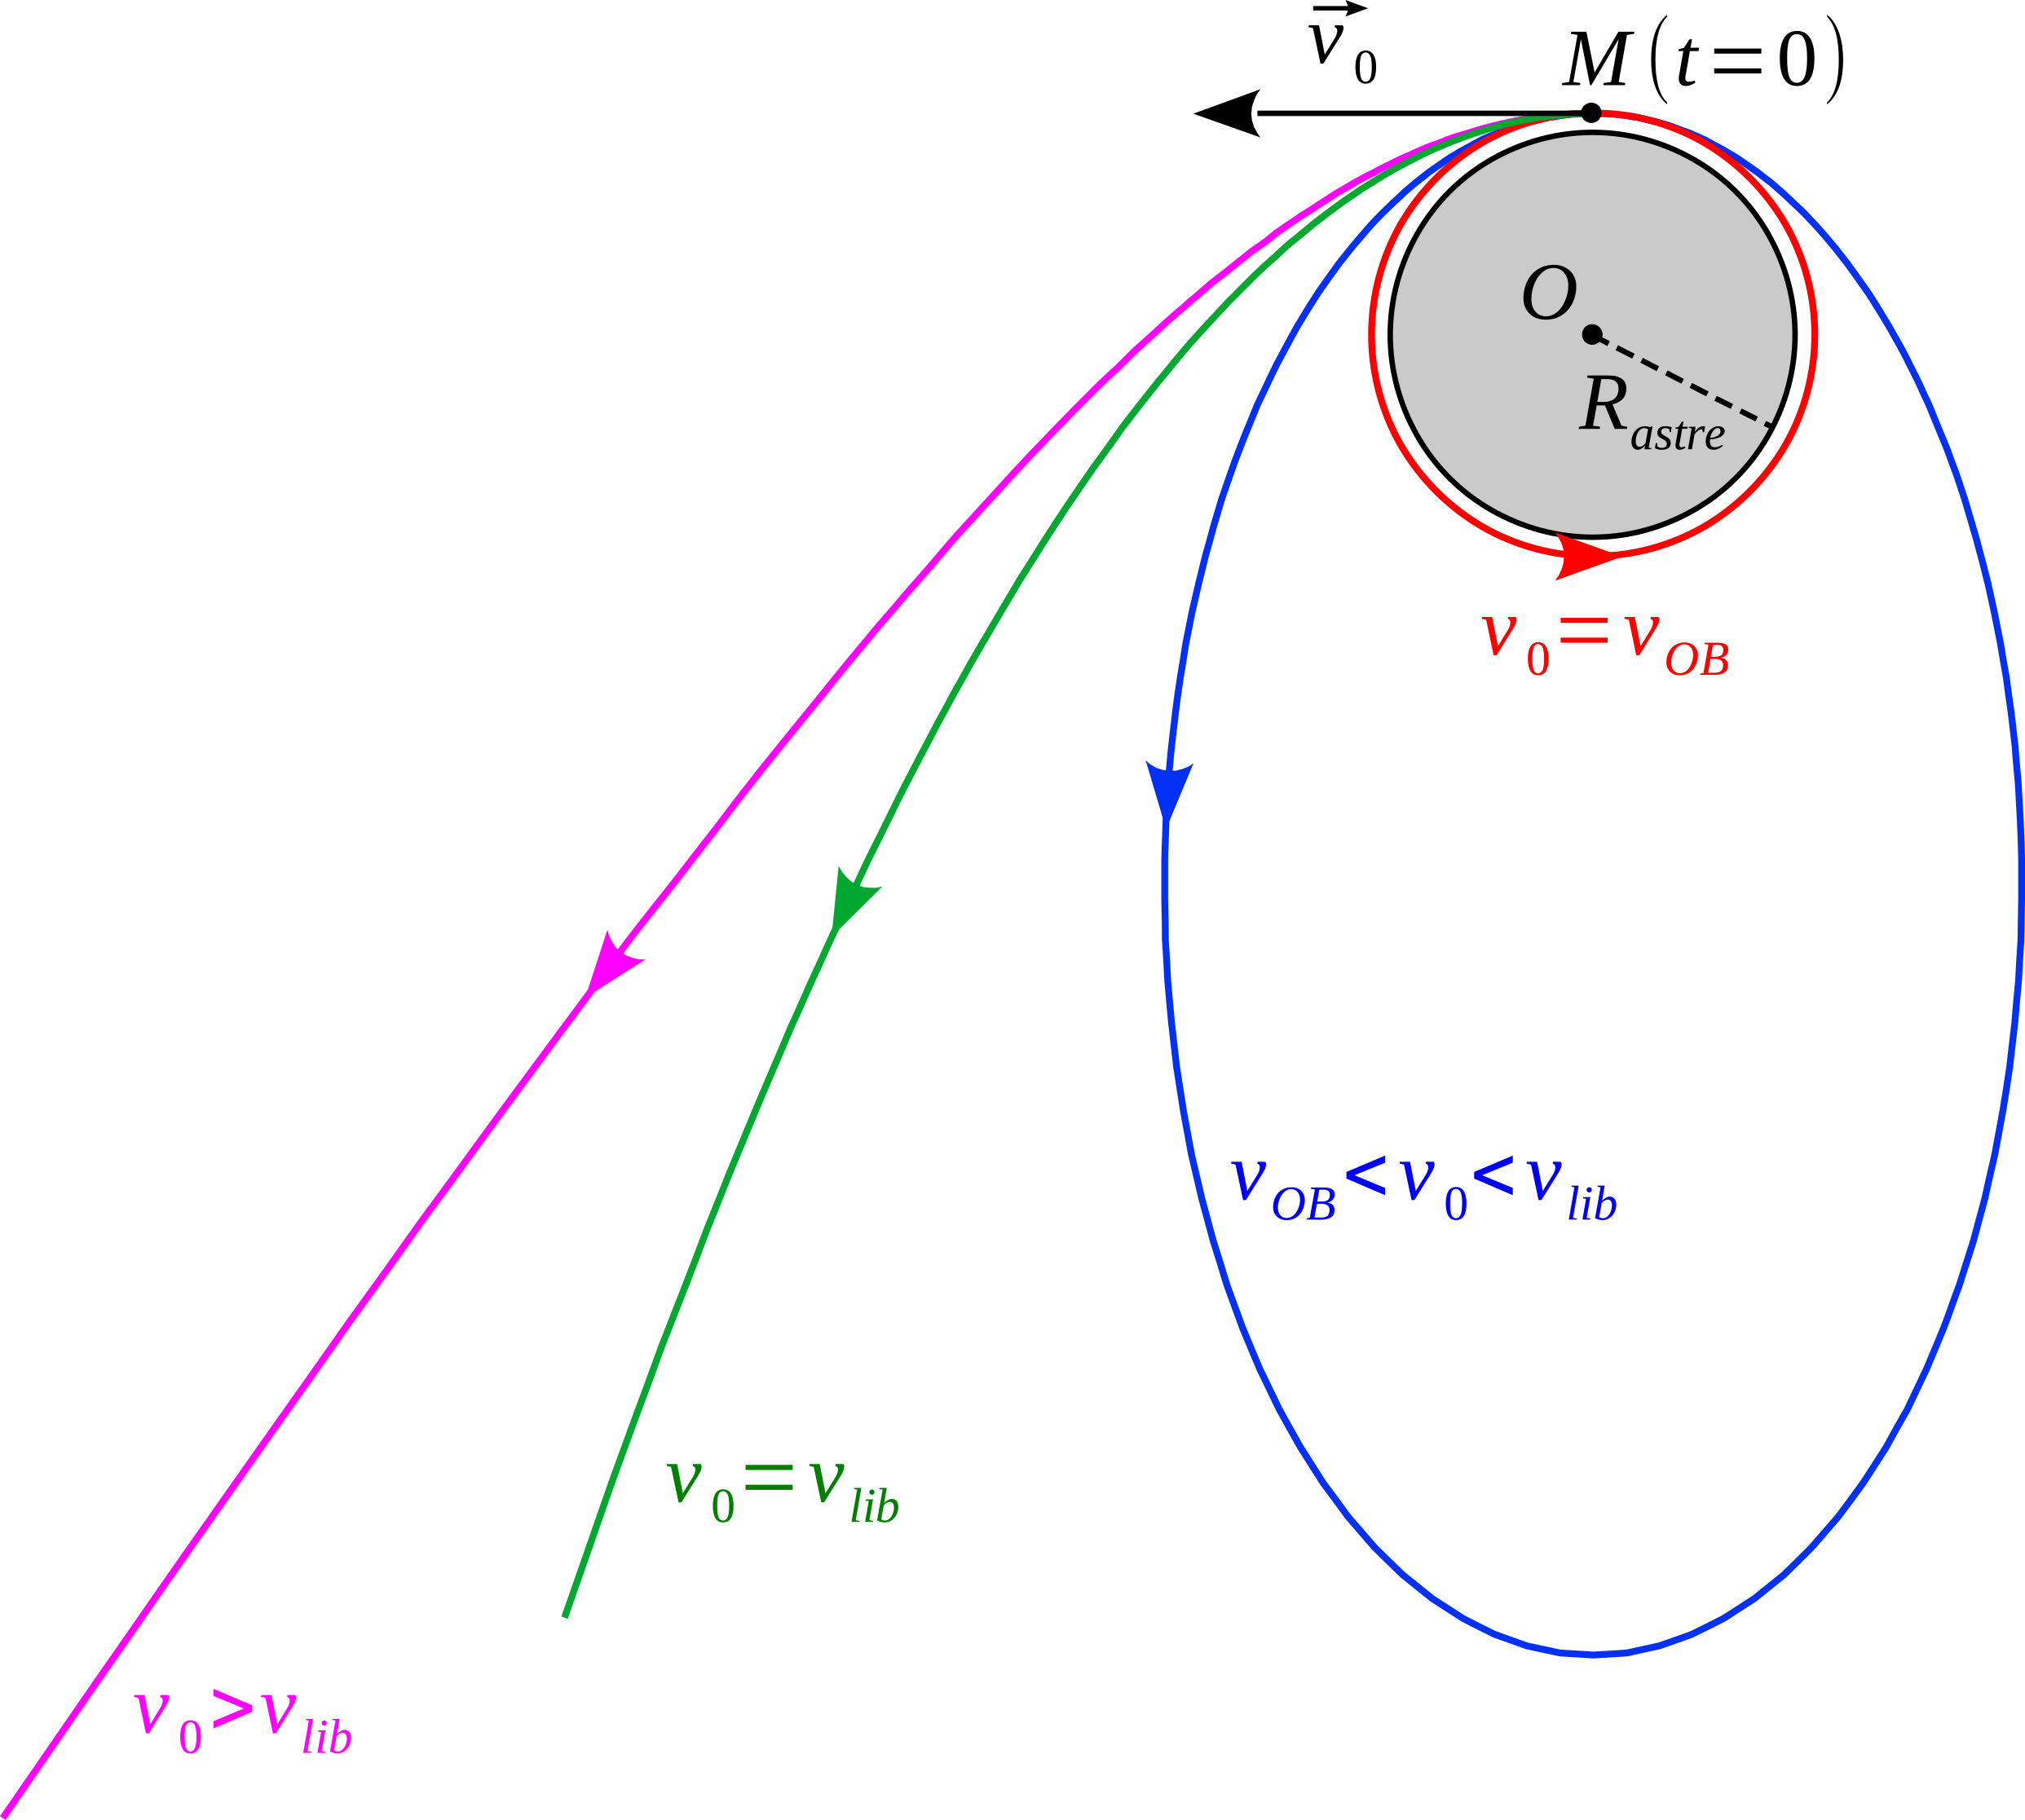
\includegraphics[scale=1]{vit_cos}
\end{center}

\subsection{Satellite géostationnaires}
\begin{tdefi}{Définition}
    Un satellite géostationnaire est un satellite qui \textbf{reste constamment
    au-dessus d'un même point} de la surface terrestre~; il apparaît donc
    immobile pour um observataire terrestre.
\end{tdefi}
Un tel système doit respecter trois conditions~:
\begin{enumerate}
    \item{Le plan de l'orbite doit être le plan de l'équateur}.
        \begin{center}
            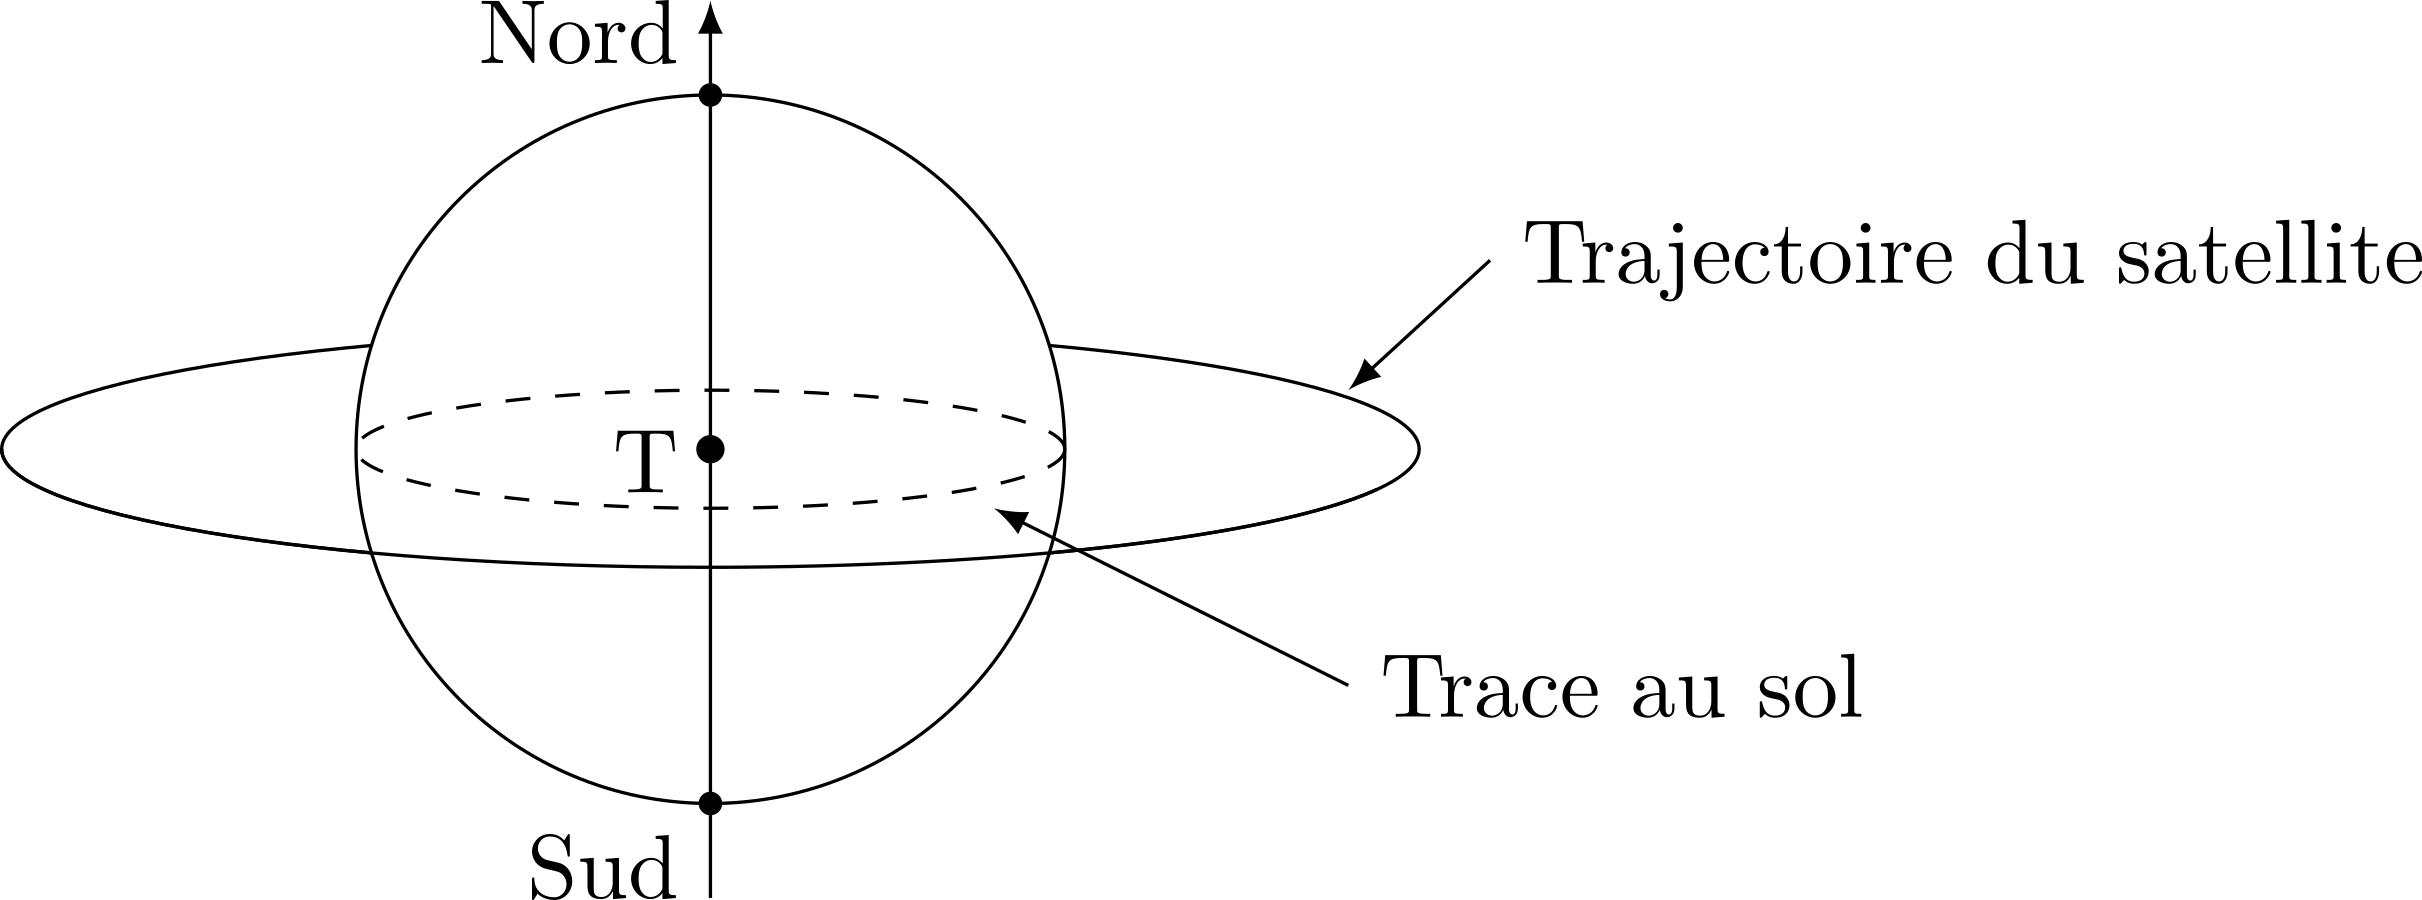
\includegraphics[scale=1]{sat_geo}
        \end{center}
        En effet, par principe de force centrale conservative, le mouvement est
        un plan passant par T le centre de la Terre. Mais comme la Terre est en
        rotation autour de l'axe de ses pôles, le seul plan contenant le centre
        de la Terre et permettant de rester immobile par rapport à sa surface
        est celui contenant l'équateur.
    \item{Le mouvement doit être synchrone avec la rotation de la Terre sur
        elle-même}. En effet d'après la raison précédente, même sur le plan de
        l'équateur il faut avoir la même vitesse angulaire $\w$, telle que
        \[\boxed{\w\ind{sat} = \tp = \w_\Ter = \frac{2\pi}{T\ind{jour}}}\]
        \danger\ Attention cependant~:
\end{enumerate}
\begin{rrema}{Remarque}
    Il existe deux durées qui peuvent s'appeler «~jour~»~:
    \begin{itemize}
        \item le \textbf{jour sidéral}, que l'on croît à tord être celui qu'on emploie
            au quotidien, et qui correspond à la durée nécessaire pour que la
            Terre effectue une rotation complète sur elle-même~; on a
            \[T\ind{sidéral} = \SI{23}{h}\,\SI{56}{min}\,\SI{04}{s}\]
        \item le \textbf{jour solaire} est l'intervalle de temps séparant deux
            passages du Soleil au zénith d'un point donné de la Terre, i.e.\ le
            temps qui sépare deux «~midis~» sur Terre~; on a
            \[T\ind{solaire} = \SI{24}{h}\]
    \end{itemize}
    Ces deux notions diffèrent légèrement à cause de la révolution de la Terre
    autour du Soleil.
    \begin{center}
        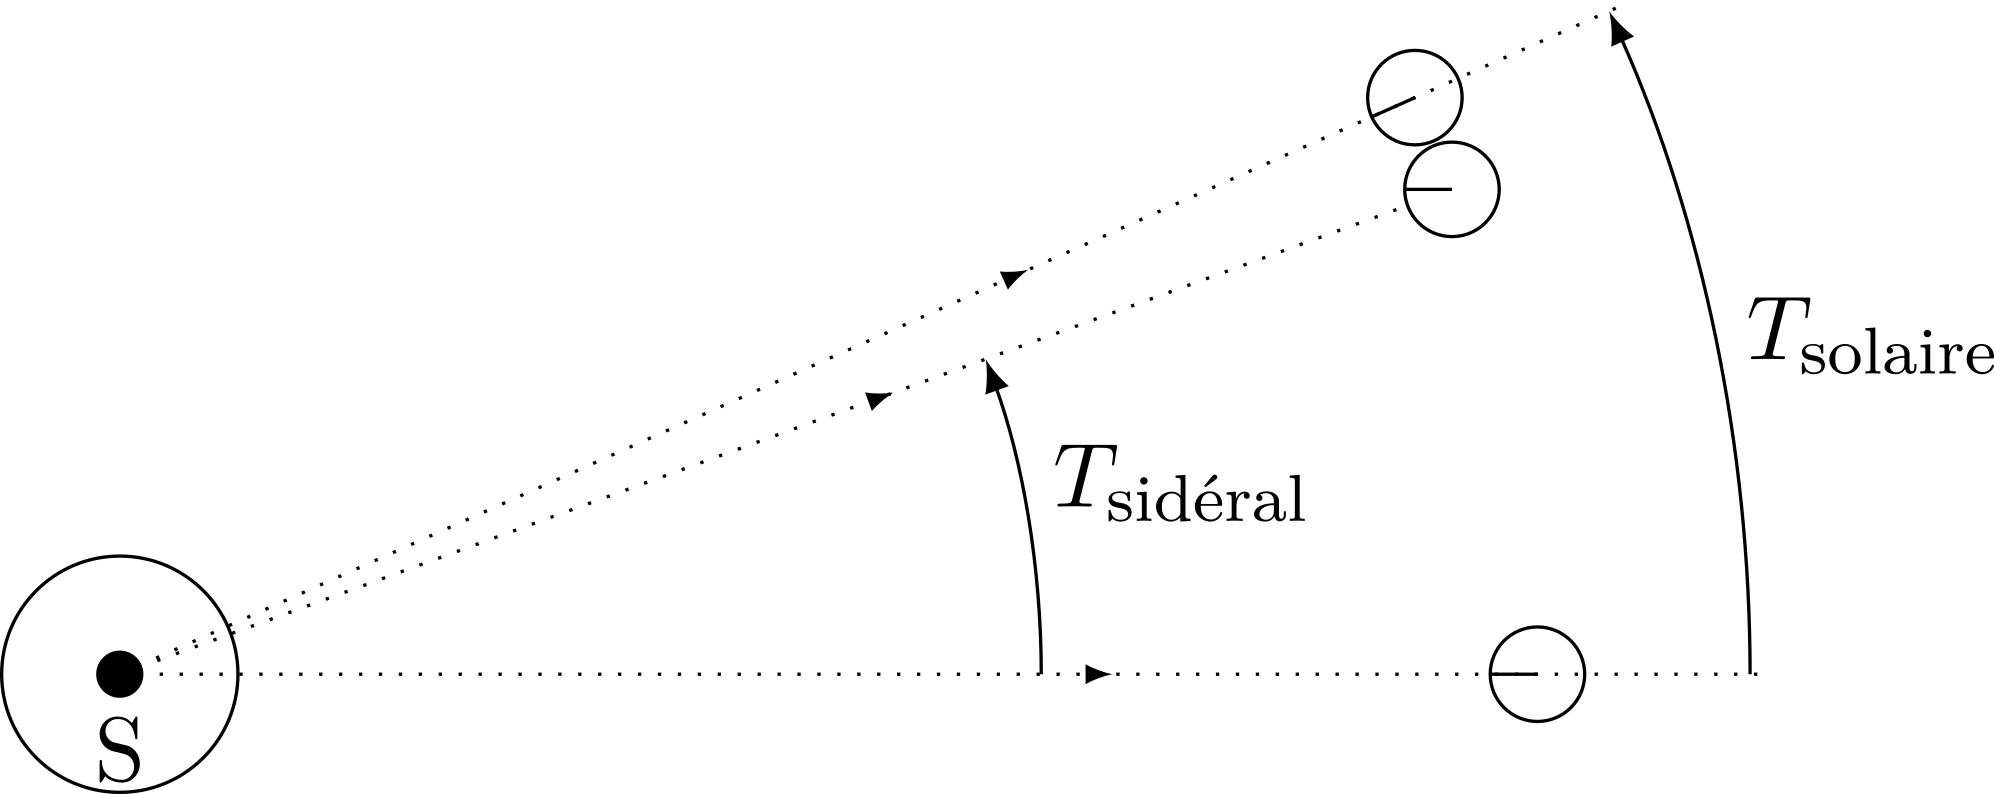
\includegraphics[scale=1]{jsid_jsol}
    \end{center}
\end{rrema}
\begin{enumerate}[resume]
    \item[] On trouve alors
        \[\w = \SI{7.2921e-5}{rad.s^{-1}}\]
    \item{Le mouvement doit être circulaire}. En effet, $C=r^2\tp$ est
        constante. Or, $\tp$ est fixe d'après ce qui précède~: ainsi, $r$ est
        fixé. On peut obtenir sa valeur avec la troisième loi de
        \textsc{Kepler}:
        \[
            \frac{T^2}{R^3} = \frac{4\pi^2}{\Gc M\ind{T}}
            \qquad
            \LRa
            \qquad
            \boxed{R = \left( \frac{\Gc M\ind{T} T^2}{4\pi^2} \right)^{1/3}}
        \]
        Il n'y a donc \textbf{qu'une seule altitude} pour les satellites
        géostationnaires, i.e. $R = \SI{42.2e6}{m}$ soit $h = \SI{35800}{km}$.
        \smallbreak
        À cette altitude, on trouve $v = R\tp = \SI{3.07}{km.s^{-1}}$.
\end{enumerate}
\end{document}
